\documentclass[final,12pt]{article}
\usepackage{epsfig}
\usepackage{graphicx}
\usepackage{makeidx}
\usepackage{upquote}
%\usepackage{showidx}
\usepackage{multicol}
\usepackage{crop}
\usepackage{amsfonts}
\usepackage{listings}
\usepackage{amsmath}
\usepackage{amssymb}
\usepackage{color}
\usepackage[usenames,dvipsnames]{xcolor}
\usepackage{courier}
\usepackage[T1]{fontenc}
%\usepackage{stmaryrd}
\usepackage{subfigure}
\usepackage{fullpage}
\usepackage[multiple]{footmisc}


\usepackage[notref,notcite,color]{showkeys}
\usepackage{xcolor,sidecap}
% js
\newcommand{\jsc}[2]{{\color{red}#1}}
\newcommand{\jsq}[1]{\textbf{\color{red}(JS: #1)}}
\usepackage{hyperref}
\hypersetup{
  colorlinks,
  linkcolor={blue!50!black},
  citecolor={red!50!black},
  urlcolor={blue!80!black}
}
%js
\renewcommand{\showkeyslabelformat}[1]{\footnotesize\ttfamily\upshape~\fbox{#1}}
\definecolor{labelkey}{rgb}{0.75,0.2,0.05}

\newcommand{\includefig}[2]{\includegraphics[width=#1\textwidth]{#2}}
\newcommand{\includeffig}[1]{\includegraphics[width=0.95\textwidth]{#1}}
\newcommand{\includehfig}[1]{\includegraphics[width=0.46\textwidth]{#1}}
\newcommand{\includetfig}[1]{\includegraphics[width=0.31\textwidth]{#1}}
\newcommand{\includefsvg}[1]{\def\svgwidth{0.95\textwidth}\input{#1}}
\newcommand{\includehsvg}[1]{\def\svgwidth{0.46\textwidth}\input{#1}}
\newcommand{\includetsvg}[1]{\def\svgwidth{0.31\textwidth}\input{#1}}
\graphicspath{{figures/}}
\newcommand{\fns}[1]{\footnotesize{#1}}
\newcommand{\scrs}[1]{{\scriptstyle{#1}}}

\newcommand{\hiddenB}{white}
\newcommand{\hiddenA}{green}

\definecolor{grey1}{rgb}{0.0,0.0,0.0}
\definecolor{grey2}{rgb}{0.2,0.2,0.2}
\definecolor{grey3}{rgb}{0.4,0.4,0.4}
\definecolor{grey4}{rgb}{0.5,0.5,0.5}

% font and color settings for font highlighting
\lstdefinestyle{highlight-fonts}{
	basicstyle=\ttfamily\mdseries\footnotesize,
	commentstyle=\ttfamily\mdseries\itshape\footnotesize,
	moredelim=[l][\color{\hiddenA}\ttfamily\mdseries\itshape\footnotesize]{\%\#},
	moredelim=[l][\color{\hiddenB}\ttfamily\mdseries\itshape\footnotesize]{\%!},
	keywordstyle=\ttfamily\mdseries\footnotesize,
	keywordstyle={[2]\ttfamily\bfseries\footnotesize},
}

% font and color settings for combined font and color highlighting
\lstdefinestyle{highlight-colors}{
	basicstyle=\color{grey1}\ttfamily\mdseries\footnotesize,
	commentstyle=\color{grey2}\ttfamily\mdseries\itshape\footnotesize,
	moredelim=[l][\color{\hiddenA}\ttfamily\mdseries\itshape\footnotesize]{\%\#},
	moredelim=[l][\color{\hiddenB}\ttfamily\mdseries\itshape\footnotesize]{\%!},
	keywordstyle=\color{grey2}\ttfamily\mdseries\footnotesize,
	keywordstyle={[2]\color{grey2}\ttfamily\bfseries\footnotesize},
}

\lstdefinestyle{gobble1}{
	xleftmargin=0.3em,
}

\lstdefinestyle{gobble2}{
	xleftmargin=-0.9em,
}

\lstdefinestyle{gobble3}{
	xleftmargin=-2.1em,
}

% import language Matlab and adjust to verbatim typesetting
\lstdefinelanguage{coco}[]{Matlab}{
	%literate={~}{{\textasciitilde}}{1},
	keywords={},
	morekeywords={},
	morekeywords=[2]{classdef,properties,private,protected,public,%
Access,Static,methods,if,function,end,for,while,else,elseif,switch,%
case,otherwise,do,repeat,until},
	otherkeywords={{,end},:end,(end,end),\{end,end\},[end,end],/private,private/},
	%morestring=[b]',
	morecomment=[l]{},
	basicstyle=\ttfamily\mdseries\footnotesize,
	commentstyle=\ttfamily\mdseries\footnotesize,
	moredelim=[l][\color{\hiddenA}\ttfamily\mdseries\footnotesize]{\%\#},
	moredelim=[l][\color{\hiddenB}\ttfamily\mdseries\footnotesize]{\%!},
	keywordstyle=\ttfamily\mdseries\footnotesize,
	keywordstyle={[2]\ttfamily\mdseries\footnotesize},
	numbers=none,
	numberstyle=\scriptsize,
	numbersep=1em,
	breaklines=false,
	breakatwhitespace=true,
	breakindent=2.5em,
	showlines=false,
	lineskip=-0.2ex,
	frame=none,
	fontadjust=true,
	columns=[c]fixed,
	basewidth={0.575em,0.45em},
	fontadjust=true,
	keepspaces=true,
	tabsize=3,
	showstringspaces=false,
	aboveskip=1.5\medskipamount,
	belowskip=1.5\medskipamount,
	xleftmargin=0.925em,
	xrightmargin=0em,
	rangeprefix={\%!},
	includerangemarker=false,
	belowcaptionskip=\bigskipamount
}

% define language with font highlighting
\lstdefinelanguage{coco-highlight-fonts}[]{coco}{
	style=highlight-fonts,
}

% define language with combined font and color highlighting
\lstdefinelanguage{coco-highlight-colors}[]{coco}{
	style=highlight-colors,
}

% use only one language for highlighting
\lstdefinelanguage{coco-highlight}[]{coco-highlight-colors}{}

\newcommand{\mcode}[1]{{\lstinline[language=coco-highlight,basewidth={0.6em,0.45em}]|#1|}}
\newcommand{\mcodes}[1]{{\lstinline[language=Matlab]|#1|}}

%\newcommand{\matlab}[1]{/Users/harrydankowicz/Documents/coco/tests/Tutorial/#1}
\newcommand{\matlab}[1]{./code/#1}

\newenvironment{exercises}{\noindent\rule[6pt]{\textwidth}{1pt}%
\vspace{-0.3cm}\subsubsection*{Exercises}\begin{enumerate}}{\end{enumerate}%
\rule[6pt]{\textwidth}{1pt}}

\setcounter{tocdepth}{3}

\begin{document}
\lstset{language=coco}

\title{Getting Started with \textsc{coco}:\\Basic Bifurcation Analysis}

\author{Harry Dankowicz \\ Department of Mechanical Science and Engineering \\
University of Illinois at Urbana-Champaign \and
Frank Schilder \\ Technical University of Denmark \and
Jan Sieber \\ College of Engineering, Mathematics
and Physical Sciences \\ University of Exeter}

\maketitle

\tableofcontents

% Activate the following line by filling in the right side. If for example the name of the root file is Main.tex, write
% "...root = Main.tex" if the chapter file is in the same directory, and "...root = ../Main.tex" if the chapter is in a subdirectory.
 
%!TEX root =  GettingStartedwithCOCO.tex

\section{Introduction}
\label{chap: intro}

This text is intended to demonstrate a level of basic usage of the \textsc{coco} software package that most students (and teachers) of nonlinear dynamics would find useful. It takes inspiration from a set of examples and demos developed by Frank Schilder for the four-day course ``Continuation Methods and \textsc{coco}'' given in conjunction with the CRITICS (Critical Transitions in Complex Systems) Winter Workshop in Barnett Hill, UK, in January 2016.

Bifurcation analysis collects techniques for characterizing the dependence of certain classes of solutions of a dynamical system to variations in problem parameters. Common examples include equilibria and periodic orbits, the number and stability of which may vary as parameters vary. Continuation techniques generate continuous families of such solutions in the combined state and parameter space, e.g., curves of periodic orbits or surfaces of equilibria. An advantage to simulation-based approaches is the ability to map out such families independently of the dynamic stability of the equilibria or periodic orbits. Bifurcation diagrams represent families of equilibria and periodic orbits as curves or surfaces in appropriate coordinate systems. Special points, such as bifurcations, are often highlighted in such diagrams.

\section{Starting \textsc{coco}}
To get started with \textsc{coco}, download the most recent release from the online repository. Make a habit of visiting this once a year in the event of minor or major upgrades. If necessary, uncompress the downloaded file and put the content in a preferred location. Navigate in \textsc{Matlab} to the folder in the \textsc{coco}  installation that contains the file \texttt{startup.m} and execute the \mcode{startup} command on the command line.
\begin{lstlisting}[language=coco-highlight,frame=lines]
>> startup
\end{lstlisting}
This adds key \textsc{coco} folders to the top of the \textsc{Matlab} search path. You can see the current search path by executing the \mcode{path} command.
\begin{lstlisting}[language=coco-highlight,frame=lines]
>> path
\end{lstlisting}
You are now ready to use \textsc{coco} according to the normal \textsc{Matlab} rules. All examples in this tutorial are included in the \textsc{coco} release in the \mcode{tutorials/Getting Started/examples} folder. Run them as is, reflect on code comments, or copy and modify for your own needs.

\section{Bifurcations of equilibria}

This section demonstrates the use of \textsc{coco} for performing continuation along families of equilibria, detecting bifurcations of equilibria, performing continuation along families of bifurcations, and visualizing the results of computation. The calling syntax is deliberately tight and mostly unexplained (but see the corresponding demos in the \textsc{coco} release).

\subsection{Detecting saddle-node points}
\label{sec: Detecting saddle-node points}
Suppose that you seek to compute a one-dimensional family of equilibria of the scalar dynamical system $\dot{x}=p-x^2$, known as the \textit{fold normal form}. Such equilibria are roots of the \textit{vector field} $f:(x,p)\mapsto p-x^2$, i.e., points in the $(x,p)$ coordinate system that lie on the curve $p=x^2$. It follows that $p\ge 0$ along this curve and that the curve folds back on itself at the \textit{saddle-node bifurcation} $x=p=0$. From $\partial_xf(x,p)=-2x$, it follows that equilibria with $x<0$ are unstable while those with $x>0$ are locally asymptotically stable.

Use \textsc{coco} to compute a discrete set of points along the curve of equilibria as follows.
\begin{lstlisting}[language=coco-highlight,frame=lines]
>> f = @(x,p) p-x.^2;
>> coco('run1', 'ode', 'isol', 'ep', f, 0.5, 'p', 1, 'p', [-1 1]);

    STEP   DAMPING               NORMS              COMPUTATION TIMES
  IT SIT     GAMMA     ||d||     ||f||     ||U||   F(x)  DF(x)  SOLVE
   0                          7.50e-01  1.50e+00    0.0    0.0    0.0
   1   1  3.56e-01  7.50e-01  4.11e-01  1.61e+00    0.0    0.0    0.0
   2   1  1.00e+00  2.68e-01  7.18e-02  1.75e+00    0.0    0.0    0.0
   3   1  1.00e+00  3.47e-02  1.20e-03  1.73e+00    0.0    0.0    0.0
   4   1  1.00e+00  6.02e-04  3.62e-07  1.73e+00    0.0    0.0    0.0
   5   1  1.00e+00  1.81e-07  3.38e-14  1.73e+00    0.0    0.0    0.0

 STEP      TIME        ||U||  LABEL  TYPE             p
    0  00:00:00   1.7321e+00      1  EP      1.0000e+00
   10  00:00:00   9.9654e-02      2          9.7411e-03
   14  00:00:00   1.3380e-06      3  FP      7.8762e-09
   14  00:00:00   1.6856e-08      4  SN      7.8780e-09
   20  00:00:00   2.1653e-01      5          4.3161e-02
   30  00:00:00   1.3657e+00      6          7.4753e-01
   31  00:00:00   1.7321e+00      7  EP      1.0000e+00
\end{lstlisting}
The screen output shows two stages of computation. First, five iterations of a \textit{Newton method} are used to converge from the (rather poor) initial solution guess $(x,p)=(0.5,1)$ to an initial equilibrium point for which $p=1$. In the fifth iteration, a problem residual, denoted by \mcode{\|\|f\|\|} evaluates to $3.38\times10^{-14}$. In the same iteration, the size of the corresponding Newton correction, denoted by \mcode{\|\|d\|\|} evaluates to $1.81\times10^{-7}$. Both are below the default tolerance threshold of $10^{-6}$, which is why the first stage terminates at this iteration. 

Next, a \textit{pseudo-arclength continuation algorithm} computes 31 additional equilibria, seven of which are captured in the screen output and labeled \mcode{1} through \mcode{7}. The number of steps of continuation is limited from above by a maximum that defaults to 100 in each direction of the curve from the initial point. This limit is not reached here, since the computation starts and ends on the boundary of the \textit{computational domain} $p\in[-1,1]$. 

Of the seven labeled points, the first and last are identified as end points (\mcode{EP}), while the third is identified as a fold point (\mcode{FP}) along the curve of equilibria and the fourth as a saddle-node bifurcation (\mcode{SN}). Although dynamical systems theory predicts that the latter two should coincide, this is only approximately true in this computation due to the use of distinct algorithms to detect the two special points.

You can visualize the results of the computation by graphing an interpolated curve through the computed equilibrium points in a two-dimensional coordinate system with $p$ along the horizontal axis and $x$ along the vertical axis, as shown below (cf.\ Fig.~\ref{fig: Section3_1_1}).
\begin{lstlisting}[language=coco-highlight,frame=lines]
>> theme = struct('special', {{'SN', 'EP'}});
>> coco_plot_bd(theme, 'run1', 'p', 'x')
\end{lstlisting}
\begin{figure}[h]
\centering
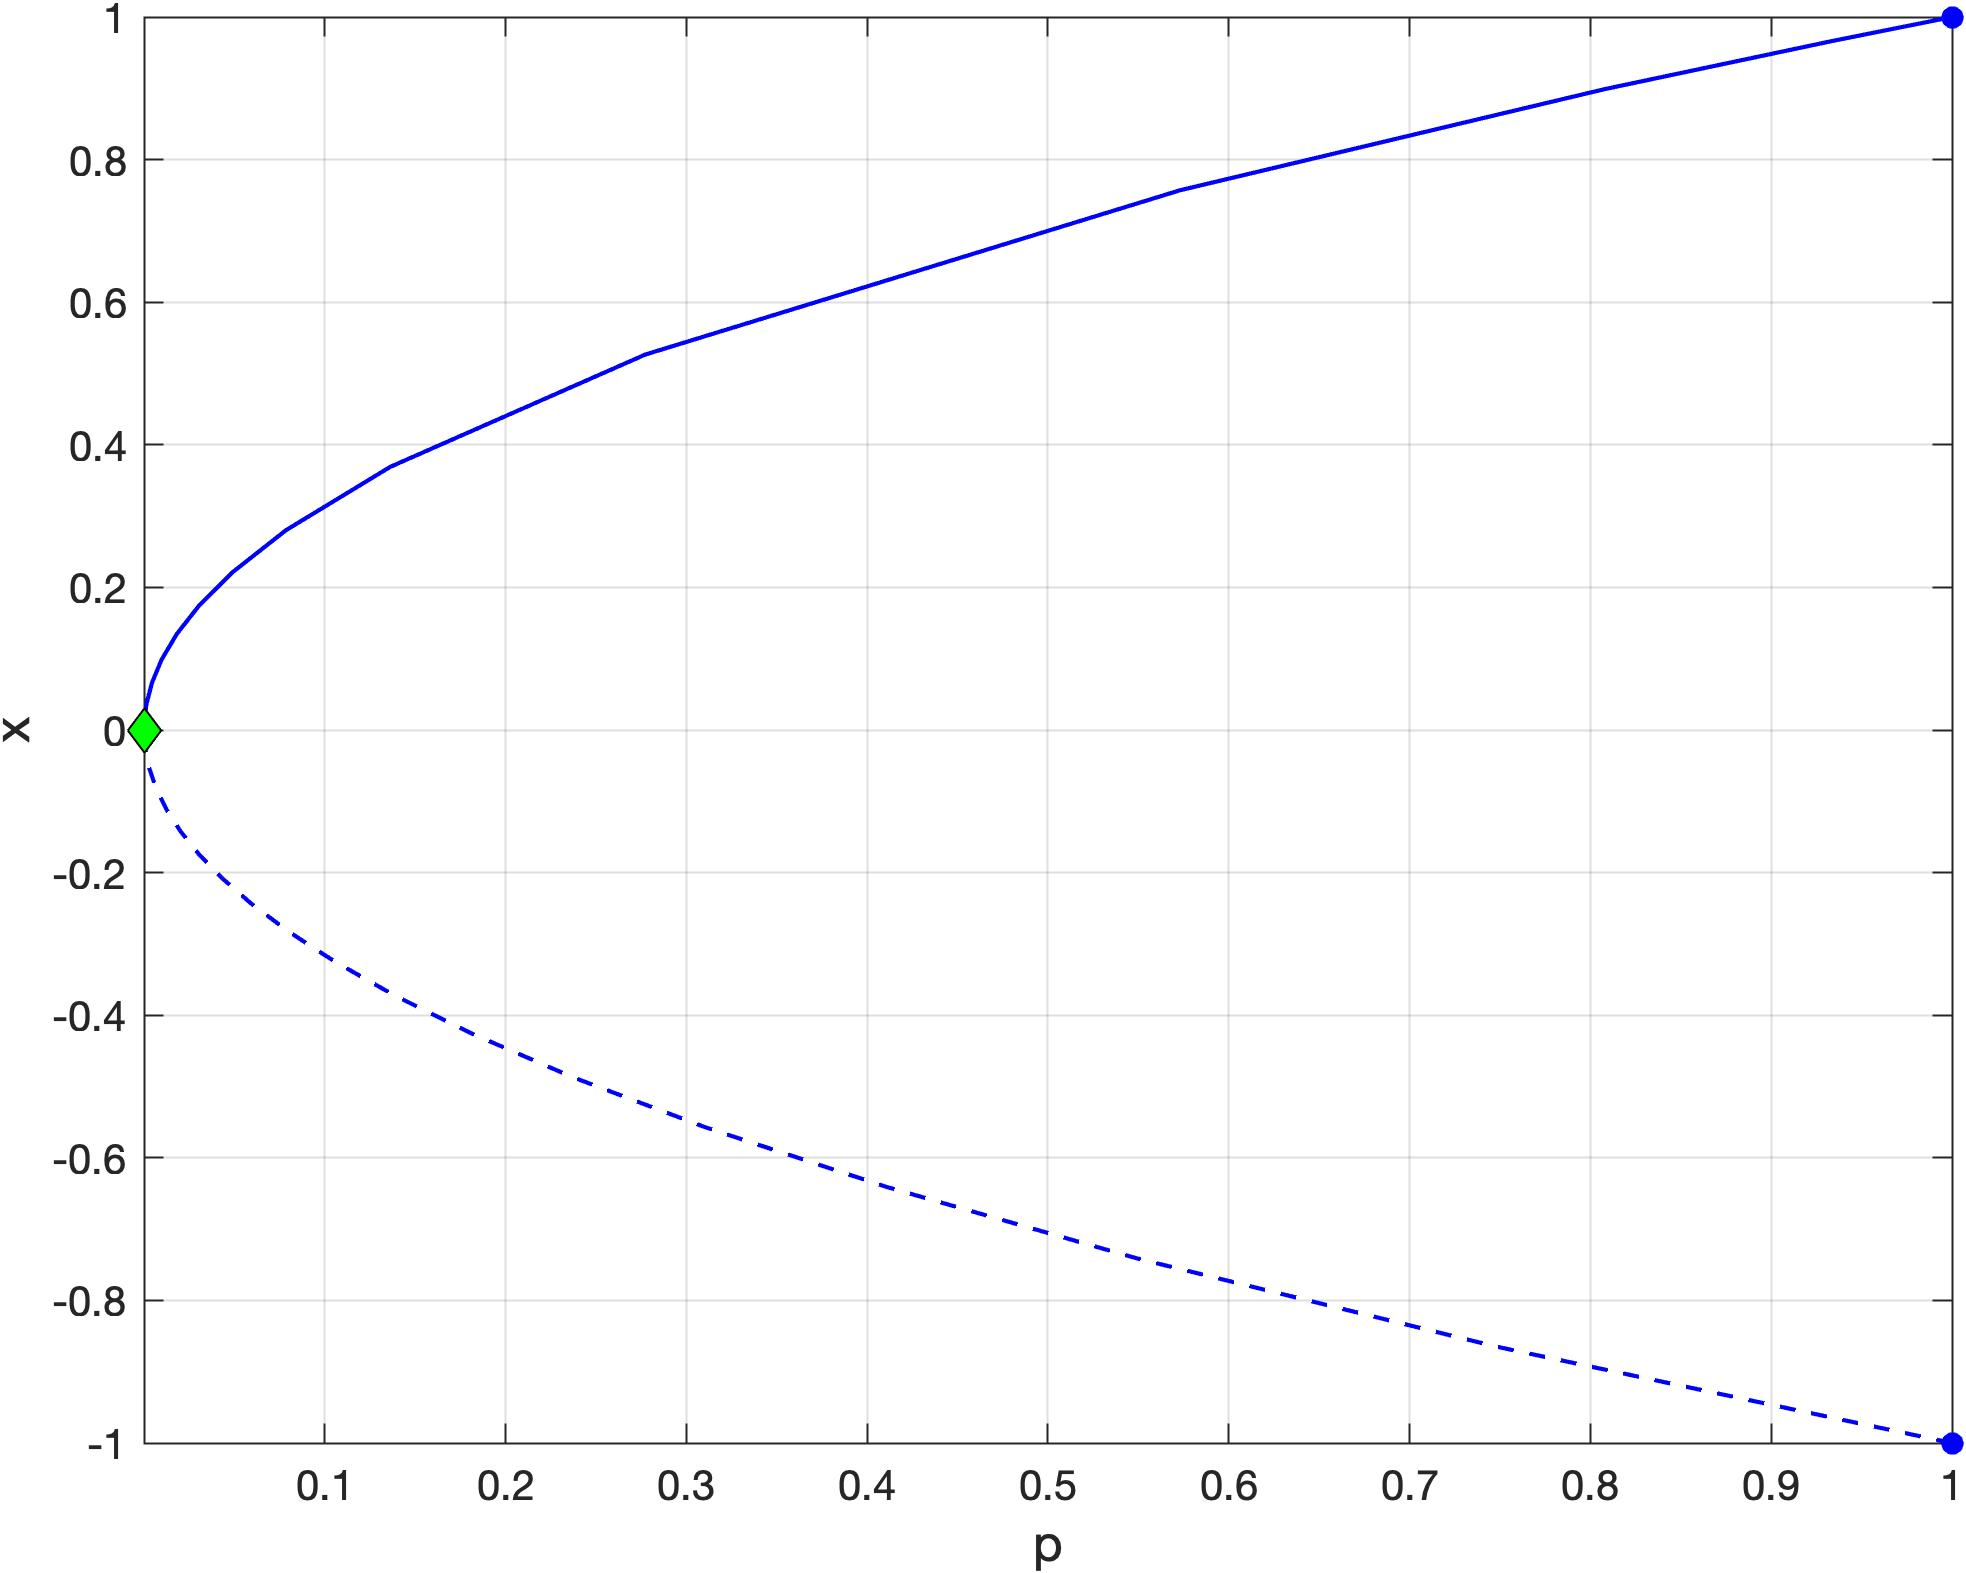
\includegraphics[width=4in]{Figures/Section3_1_1.jpg}
\caption{Bifurcation diagram showing branches of asymptotically stable (solid) and unstable (dashed) equilibria for the vector field in Section~\ref{sec: Detecting saddle-node points}. The green diamond marks a saddle-node bifurcation while the small blue disks mark the end points of the computation.}
\label{fig: Section3_1_1}
\end{figure}
The output distinguishes between portions of the curve representing stable and unstable equilibria and includes markers highlighting the \mcode{EP} and \mcode{SN} points.

\subsection{Detecting branch points}
\label{sec: Detecting branch points}
There exists a single curve of equilibria for the fold normal form. For the \textit{transcritical normal form} $\dot{x}=px-x^2$, equilibria correspond to points on the two curves $x=0$ and $p=x$. These intersect at a \textit{transcritical bifurcation} at $x=p=0$. From $\partial_xf(x,p)=p-2x$, it follows that equilibria along $x=0$ are locally asymptotically stable for $p<0$ and unstable for $p>0$, while the reverse holds along $p=x$.

You can use \textsc{coco} to compute a discrete set of points along the first curve of equilibria.
\begin{lstlisting}[language=coco-highlight,frame=lines]
>> f = @(x,p) p.*x-x.^2;
>> coco('run1', 'ode', 'isol', 'ep', f, 0, 'p', -1, 'p', [-1 1]);

    STEP   DAMPING               NORMS              COMPUTATION TIMES
  IT SIT     GAMMA     ||d||     ||f||     ||U||   F(x)  DF(x)  SOLVE
   0                          0.00e+00  1.41e+00    0.0    0.0    0.0

 STEP      TIME        ||U||  LABEL  TYPE             p
    0  00:00:00   1.4142e+00      1  EP     -1.0000e+00
    5  00:00:00   2.2484e-07      2  SN      1.5899e-07
    5  00:00:00   2.2484e-07      3  BP      1.5899e-07
    8  00:00:00   1.4142e+00      4  EP      1.0000e+00
\end{lstlisting}
In this case, the first stage of computation terminates immediately, since the initial solution guess $(x,p)=(0,-1)$ lies on the curve $x=0$. In the second stage, the continuation algorithm computes 8 additional equilibria. Of the equilibria labeled \mcode{1} through \mcode{4}, the first and last are again identified as end points (\mcode{EP}), while the second and third are identified as a saddle-node bifurcation (\mcode{SN}) and branch point (\mcode{BP}), respectively, and approximately coincide with the origin. The characterization of this point as a saddle-node bifurcation is of course contrary to dynamical systems theory, but reflects the default behavior of the detection algorithm.

You can continue from the \mcode{BP} point along the second curve of equilibria as follows.
\begin{lstlisting}[language=coco-highlight,frame=lines]
>> BP = coco_bd_labs('run1', 'BP');
>> coco('run2', 'ode', 'BP', 'ep', 'run1', BP, 'p', [-1 1]);

STEP      TIME        ||U||  LABEL  TYPE             p
    0  00:00:00   2.2484e-07      1  EP      1.5899e-07
    7  00:00:00   1.7321e+00      2  EP     -1.0000e+00

 STEP      TIME        ||U||  LABEL  TYPE             p
    0  00:00:00   2.2484e-07      3  EP      1.5899e-07
    1  00:00:00   6.8132e-07      4  BP      4.6035e-07
    1  00:00:00   9.7048e-07      5  SN      6.4659e-07
    7  00:00:00   1.7321e+00      6  EP      1.0000e+00
\end{lstlisting}
In this case, there is no first stage of computation (since the branch point is a singularity), and the second stage proceeds in two opposite directions along the curve $p=x$. To visualize the two curves of equilibria, use the \mcode{coco_plot_bd} command twice (cf.\ Fig.~\ref{fig: Section3_2_1}).
\begin{lstlisting}[language=coco-highlight,frame=lines]
>> clf
>> hold on
>> theme1 = struct('special', {{'BP', 'EP'}});
>> coco_plot_bd(theme1, 'run1', 'p', 'x')
>> theme2 = struct('special', {{'EP'}});
>> coco_plot_bd(theme2, 'run2', 'p', 'x')
>> hold off
>> axis tight
>> grid on
\end{lstlisting}
\begin{figure}[h]
\centering
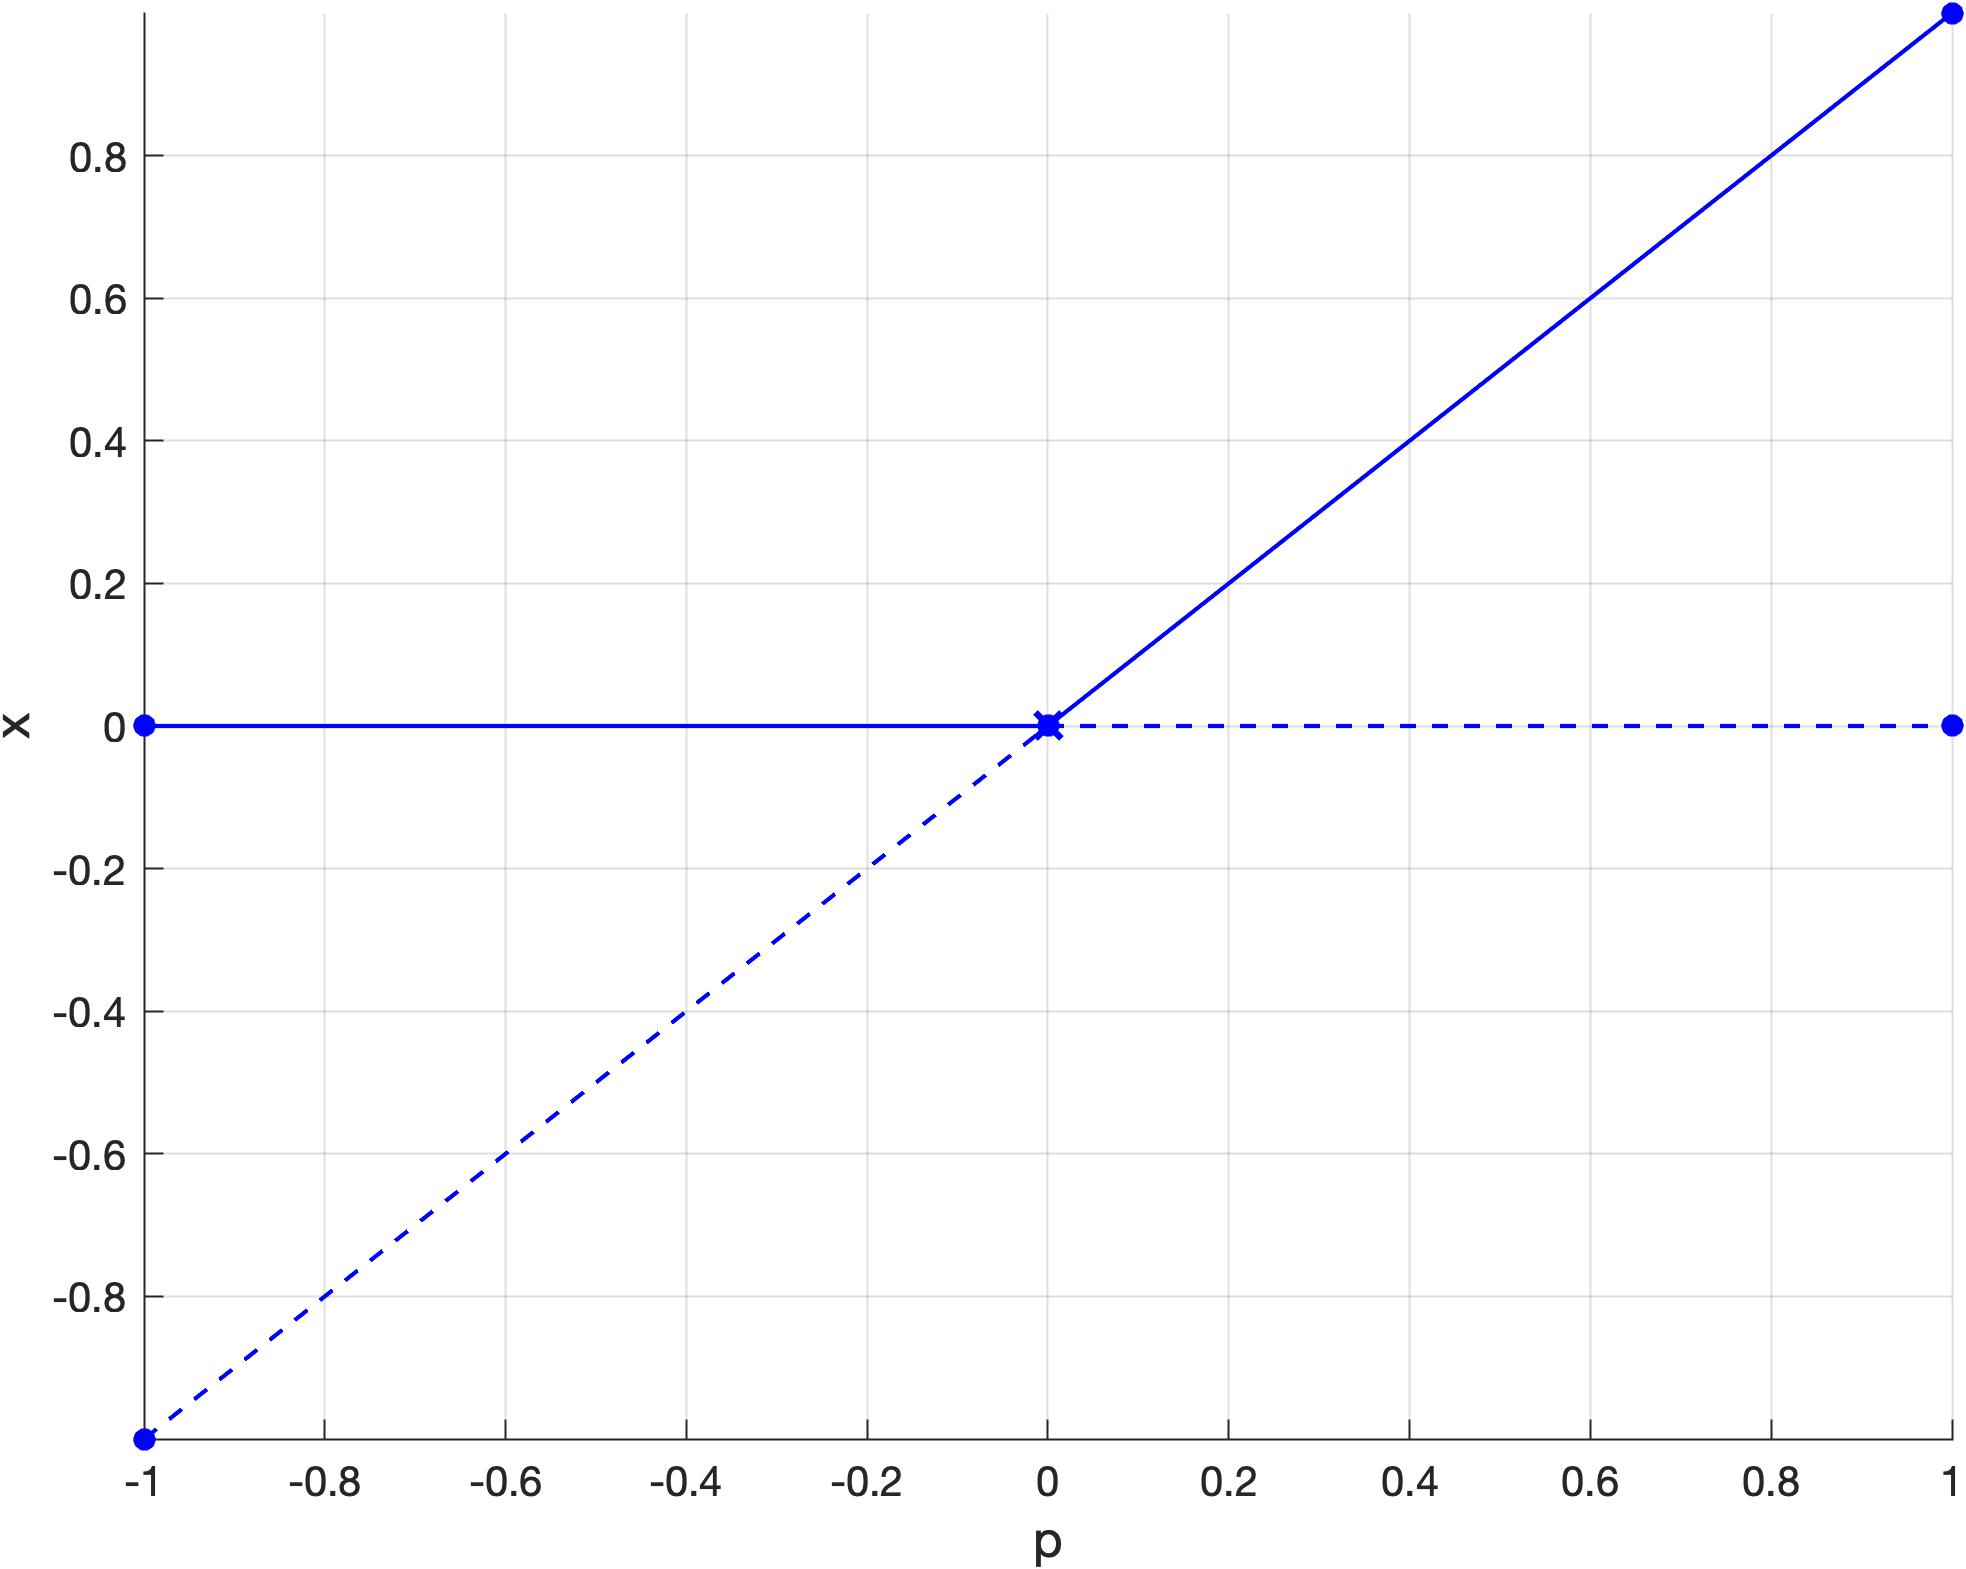
\includegraphics[width=4in]{Figures/Section3_2_1.jpg}
\caption{Bifurcation diagram showing branches of asymptotically stable (solid) and unstable (dashed) equilibria for the vector field in Section~\ref{sec: Detecting branch points}. The blue cross marks a branch point while the small blue disks mark the end points of each computation.}
\label{fig: Section3_2_1}
\end{figure}

\subsection{Continuing saddle-node points}
\label{sec: Continuing saddle-node points}
As a third example, consider the \textit{pitchfork normal form} $\dot{x}=\kappa+x(\lambda-x^2)$ in the two problem parameters $\lambda$ and $\kappa$. Equilibria lie on the two-dimensional surface $\kappa=x(x^2-\lambda)$ which includes the curves $s\mapsto (0,s,0)$, $s\mapsto (s,s^2,0)$, $s\mapsto (s,1/2,s(s^2-1/2))$, and $s\mapsto (s,3s^2,-2s^3)$ in the $(x,\lambda,\kappa)$ coordinate system. The first two of these intersect at a \textit{pitchfork bifurcation} at $x=\lambda=\kappa=0$, while the fourth curve consists entirely of saddle-node bifurcations and intersects the third curve when $s^2=1/6$. The fourth curve passes through the origin in a fold point known as a \textit{cusp bifurcation}.

To compute the four curves with \textsc{coco}, use the following sequence of commands.
\begin{lstlisting}[language=coco-highlight,frame=lines]
>> f = @(x,p) p(2,:)+x.*(p(1,:)-x.^2);
>> coco('run1', 'ode', 'isol', 'ep', ...
     f, 0, {'la' 'ka'}, [-2; 0], 'la', [-2 2])

    STEP   DAMPING               NORMS              COMPUTATION TIMES
  IT SIT     GAMMA     ||d||     ||f||     ||U||   F(x)  DF(x)  SOLVE
   0                          0.00e+00  2.83e+00    0.0    0.0    0.0

 STEP      TIME        ||U||  LABEL  TYPE            la
    0  00:00:00   2.8284e+00      1  EP     -2.0000e+00
    8  00:00:00   6.4118e-07      2  SN      4.5339e-07
    8  00:00:00   6.4118e-07      3  BP      4.5339e-07
   10  00:00:00   1.3226e+00      4          9.3520e-01
   14  00:00:00   2.8284e+00      5  EP      2.0000e+00

>> BP = coco_bd_labs('run1', 'BP');
>> coco(prob, 'run2', 'ode', 'BP', 'ep', ...
     'run1', BP, 'la', [-2 2]);

 STEP      TIME        ||U||  LABEL  TYPE            la
    0  00:00:00   6.4118e-07      1  EP      4.5339e-07
    1  00:00:00   3.0228e-06      2  SN     -2.3840e-10
    1  00:00:00   2.8974e-03      3  FP     -1.8413e-04
   10  00:00:00   2.8084e-01      4          6.9276e-02
   20  00:00:00   2.0444e+00      5          1.2170e+00
   23  00:00:00   3.1623e+00      6  EP      2.0000e+00

 STEP      TIME        ||U||  LABEL  TYPE            la
    0  00:00:00   6.4118e-07      7  EP      4.5339e-07
    1  00:00:00   6.8665e-07      8  BP      4.7487e-07
    1  00:00:00   3.4690e-02      9  SN      1.2015e-03
   10  00:00:00   6.4635e-01     10          2.7095e-01
   18  00:00:01   3.1623e+00     11  EP      2.0000e+00

>> coco(prob, 'run3', 'ode', 'isol', 'ep', ...
     f, 0, {'la' 'ka'}, [0.5; 0], 'ka', [-2 2]);

    STEP   DAMPING               NORMS              COMPUTATION TIMES
  IT SIT     GAMMA     ||d||     ||f||     ||U||   F(x)  DF(x)  SOLVE
   0                          0.00e+00  5.00e-01    0.0    0.0    0.0

 STEP      TIME        ||U||  LABEL  TYPE            ka
    0  00:00:00   5.0000e-01      1  EP      0.0000e+00
    6  00:00:00   6.7357e-01      2  FP     -1.3608e-01
    6  00:00:00   6.7358e-01      3  SN     -1.3608e-01
   10  00:00:00   7.3824e-01      4         -1.2073e-01
   20  00:00:00   9.4972e-01      5          1.0362e-01
   28  00:00:00   3.1917e+00      6  EP      2.0000e+00

 STEP      TIME        ||U||  LABEL  TYPE            ka
    0  00:00:00   5.0000e-01      7  EP      0.0000e+00
    6  00:00:00   6.7357e-01      8  FP      1.3608e-01
    6  00:00:00   6.7358e-01      9  SN      1.3608e-01
   10  00:00:00   7.3824e-01     10          1.2073e-01
   20  00:00:01   9.4972e-01     11         -1.0362e-01
   28  00:00:01   3.1917e+00     12  EP     -2.0000e+00

>> SN = coco_bd_labs('run3', 'SN');
>> coco(prob, 'run4', 'ode', 'SN', 'SN', ...
     'run3', SN(1), {'la' 'ka'}, {[-2 2] [-2 2]})

    STEP   DAMPING               NORMS              COMPUTATION TIMES
  IT SIT     GAMMA     ||d||     ||f||     ||U||   F(x)  DF(x)  SOLVE
   0                          5.07e-08  1.31e+00    0.0    0.0    0.0

 STEP      TIME        ||U||  LABEL  TYPE            la           ka
    0  00:00:00   1.3053e+00      1  EP      5.0000e-01  -1.3608e-01
   10  00:00:00   1.0007e+00      2          4.3387e-03  -1.1000e-04
   14  00:00:00   1.0000e+00      3  FP      9.4219e-09   1.0483e-11
   20  00:00:00   1.0023e+00      4          1.2647e-02   5.4743e-04
   30  00:00:00   1.0722e+00      5          2.0057e-01   3.4574e-02
   40  00:00:01   3.4694e+00      6  EP      2.0000e+00   1.0887e+00

 STEP      TIME        ||U||  LABEL  TYPE            la           ka
    0  00:00:01   1.3053e+00      7  EP      5.0000e-01  -1.3608e-01
    7  00:00:01   3.4694e+00      8  EP      2.0000e+00  -1.0887e+00
\end{lstlisting}
The second and fourth curves are here obtained by restarting continuation from a \mcode{BP} and \mcode{SN} point, respectively, found in the preceding run. The four curves may be visualized simultaneously using the following commands (cf.\ Fig.~\ref{fig: Section3_3_1}).
\begin{lstlisting}[language=coco-highlight,frame=lines]
>> clf
>> theme1 = struct('special', {{'BP', 'EP'}});
>> theme2 = struct('special', {{'EP'}});
>> theme3 = struct('special', {{'SN', 'EP'}});
>> hold on
>> coco_plot_bd(theme1, 'run1', 'la', 'ka', 'x')
>> coco_plot_bd(theme2, 'run2', 'la', 'ka', 'x')
>> coco_plot_bd(theme3, 'run3', 'la', 'ka', 'x')
>> coco_plot_bd(theme2, 'run4', 'la', 'ka', 'x')
>> hold off
>> axis tight
>> grid on
>> view(-15,25)
\end{lstlisting}
\begin{figure}[h]
\centering
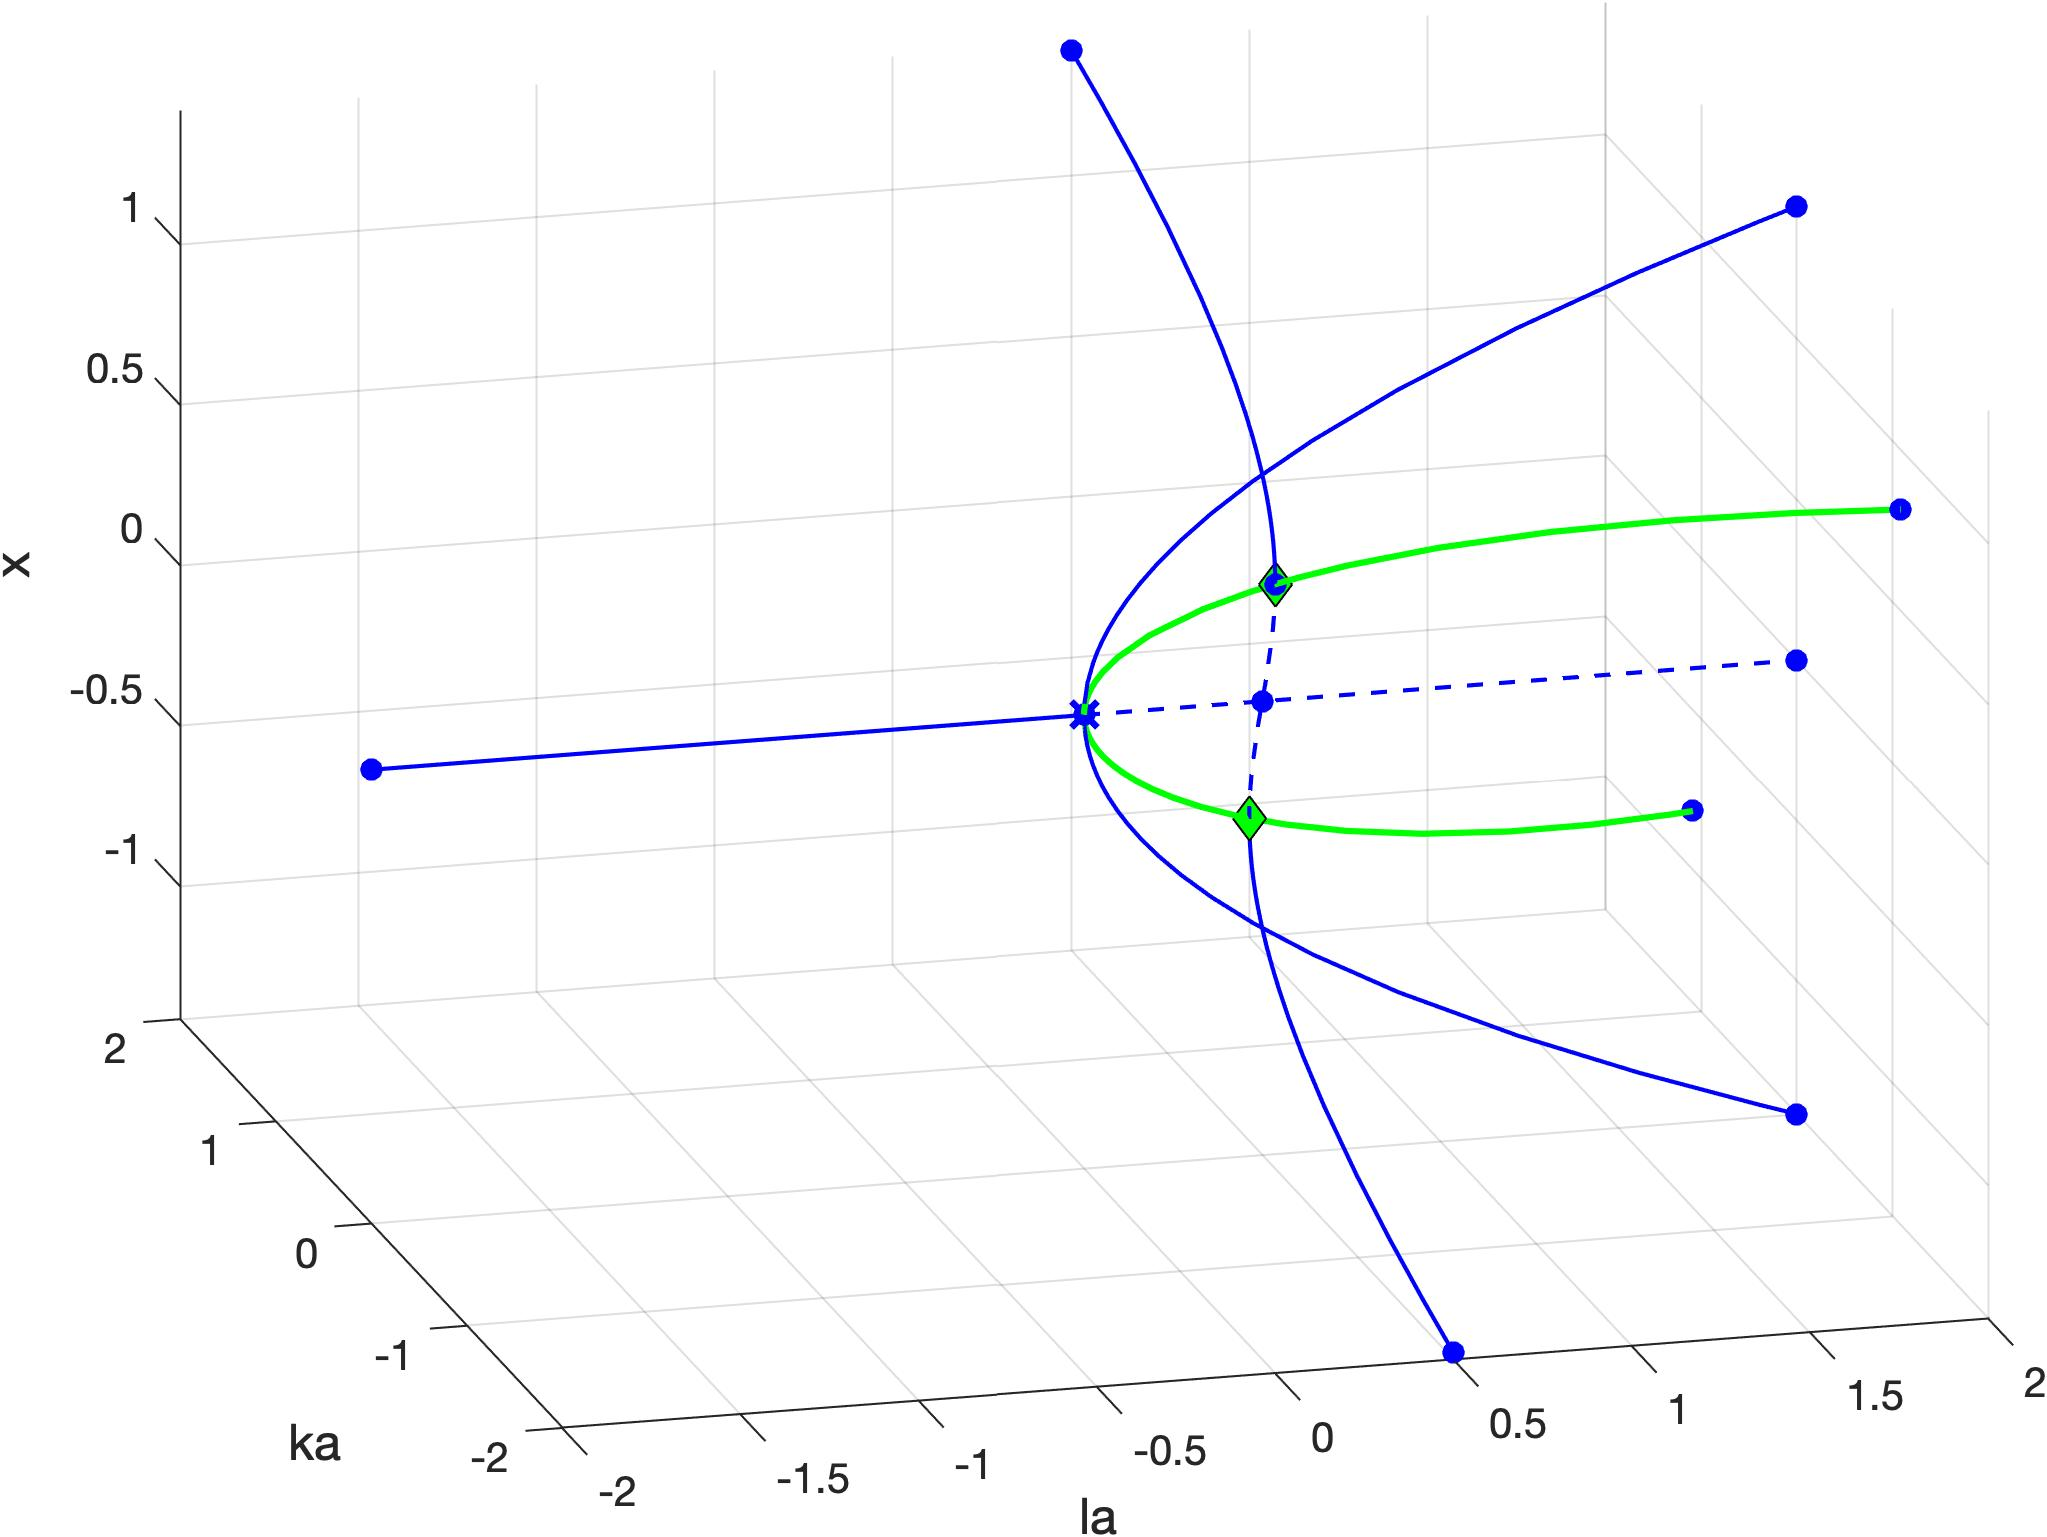
\includegraphics[width=4in]{Figures/Section3_3_1.jpg}
\caption{Bifurcation diagram showing branches of asymptotically stable (blue solid) and unstable (blue dashed) equilibria and saddle-node bifurcations (solid green) for the vector field in Section~\ref{sec: Continuing saddle-node points}. The blue cross marks a branch point, the green diamonds mark saddle-node bifurcations, and the small blue disks mark the end points of each computation.}
\label{fig: Section3_3_1}
\end{figure}
As with all examples in this tutorial, the visualization is best inspected in a \textsc{Matlab} figure window.

\subsection{Continuing Hopf bifurcations}
\label{sec: Continuing Hopf bifurcations}
Next, consider a so-called Brusselator model described by the vector field 
\[
f(x,p)=\begin{pmatrix}A-x_1(B-x_1x_2)-x_1\\x_1(B-x_1x_2)\end{pmatrix}
\]
in terms of the vector of state variables $x=(x_1,x_2)\in\mathbb{R}^2$ and vector of problem parameters $p=(A,B)\in\mathbb{R}^2$, and encoded in the \mcode{brus} function shown below.
\begin{lstlisting}[language=coco-highlight,frame=shadowbox]
function f = brus(x,p)

A  = p(1,:);
B  = p(2,:);
x1 = x(1,:);
x2 = x(2,:);

BB = x1.*(B - x1.*x2);

f(1,:) = A - BB - x1;
f(2,:) = BB;

end
\end{lstlisting}
Equilibria are found on the two surfaces $A=x_1=0$ and $A=x_1,\,B=x_1x_2$. The latter includes the curves $s\mapsto (1,s,1,s)$ and $s\mapsto(s,(1+s^2)/s,s,1+s^2)$ in the $(x_1,x_2,A,B)$ coordinate system. The second of these consists of \textit{Hopf bifurcations}. The two curves may be computed with \textsc{coco} as follows.
\begin{lstlisting}[language=coco-highlight,frame=lines]
>> coco('run1', 'ode', 'isol', 'ep', ...
     @brus, [1; 0], {'A' 'B'}, [1; 0], 'B', [0 3]);

    STEP   DAMPING               NORMS              COMPUTATION TIMES
  IT SIT     GAMMA     ||d||     ||f||     ||U||   F(x)  DF(x)  SOLVE
   0                          0.00e+00  1.41e+00    0.0    0.0    0.0

 STEP      TIME        ||U||  LABEL  TYPE             B
    0  00:00:00   1.4142e+00      1  EP      0.0000e+00
    9  00:00:00   3.7417e+00      2  HB      2.0000e+00
   10  00:00:00   4.3853e+00      3          2.3966e+00
   13  00:00:00   5.3852e+00      4  EP      3.0000e+00

>> HB = coco_bd_labs('run1', 'HB');
>> coco('run2', 'ode', 'HB', 'HB', ...
     'run1', HB(1), {'A' 'B'}, {[] [0 3]});

    STEP   DAMPING               NORMS              COMPUTATION TIMES
  IT SIT     GAMMA     ||d||     ||f||     ||U||   F(x)  DF(x)  SOLVE
   0                          1.32e-07  4.29e+00    0.0    0.0    0.0

 STEP      TIME        ||U||  LABEL  TYPE             A            B
    0  00:00:00   4.2895e+00      1  EP      1.0000e+00   2.0000e+00
   10  00:00:00   3.3815e+00      2          5.1142e-01   1.2616e+00
   20  00:00:00   4.7582e+00      3          2.4401e-01   1.0595e+00
   30  00:00:01   9.5180e+00      4          1.0840e-01   1.0117e+00
   40  00:00:01   1.4452e+01      5          7.0111e-02   1.0049e+00
   50  00:00:01   1.9421e+01      6          5.1864e-02   1.0027e+00
   60  00:00:02   2.4403e+01      7          4.1166e-02   1.0017e+00
   70  00:00:02   2.9391e+01      8          3.4131e-02   1.0012e+00
   80  00:00:02   3.4383e+01      9          2.9151e-02   1.0008e+00
   90  00:00:02   3.9376e+01     10          2.5440e-02   1.0006e+00
  100  00:00:03   4.4371e+01     11  EP      2.2568e-02   1.0005e+00

 STEP      TIME        ||U||  LABEL  TYPE             A            B
    0  00:00:03   4.2895e+00     12  EP      1.0000e+00   2.0000e+00
    7  00:00:03   6.2849e+00     13  EP      1.4142e+00   3.0000e+00
\end{lstlisting}
The following sequence of commands visualizes the result (cf.\ Fig.~\ref{fig: Section3_4_1}).
\begin{lstlisting}[language=coco-highlight,frame=lines]
>> clf
>> hold on
>> theme1 = struct('special', {{'HB', 'EP'}});
>> theme2 = struct('special', {{'EP'}});
>> coco_plot_bd(theme1, 'run1', 'B', 'A', '||x||_2')
>> coco_plot_bd(theme2, 'run2', 'B', 'A', '||x||_2')
>> hold off
>> axis tight
>> grid on
>> view(-65,40)
\end{lstlisting}
\begin{figure}[h]
\centering
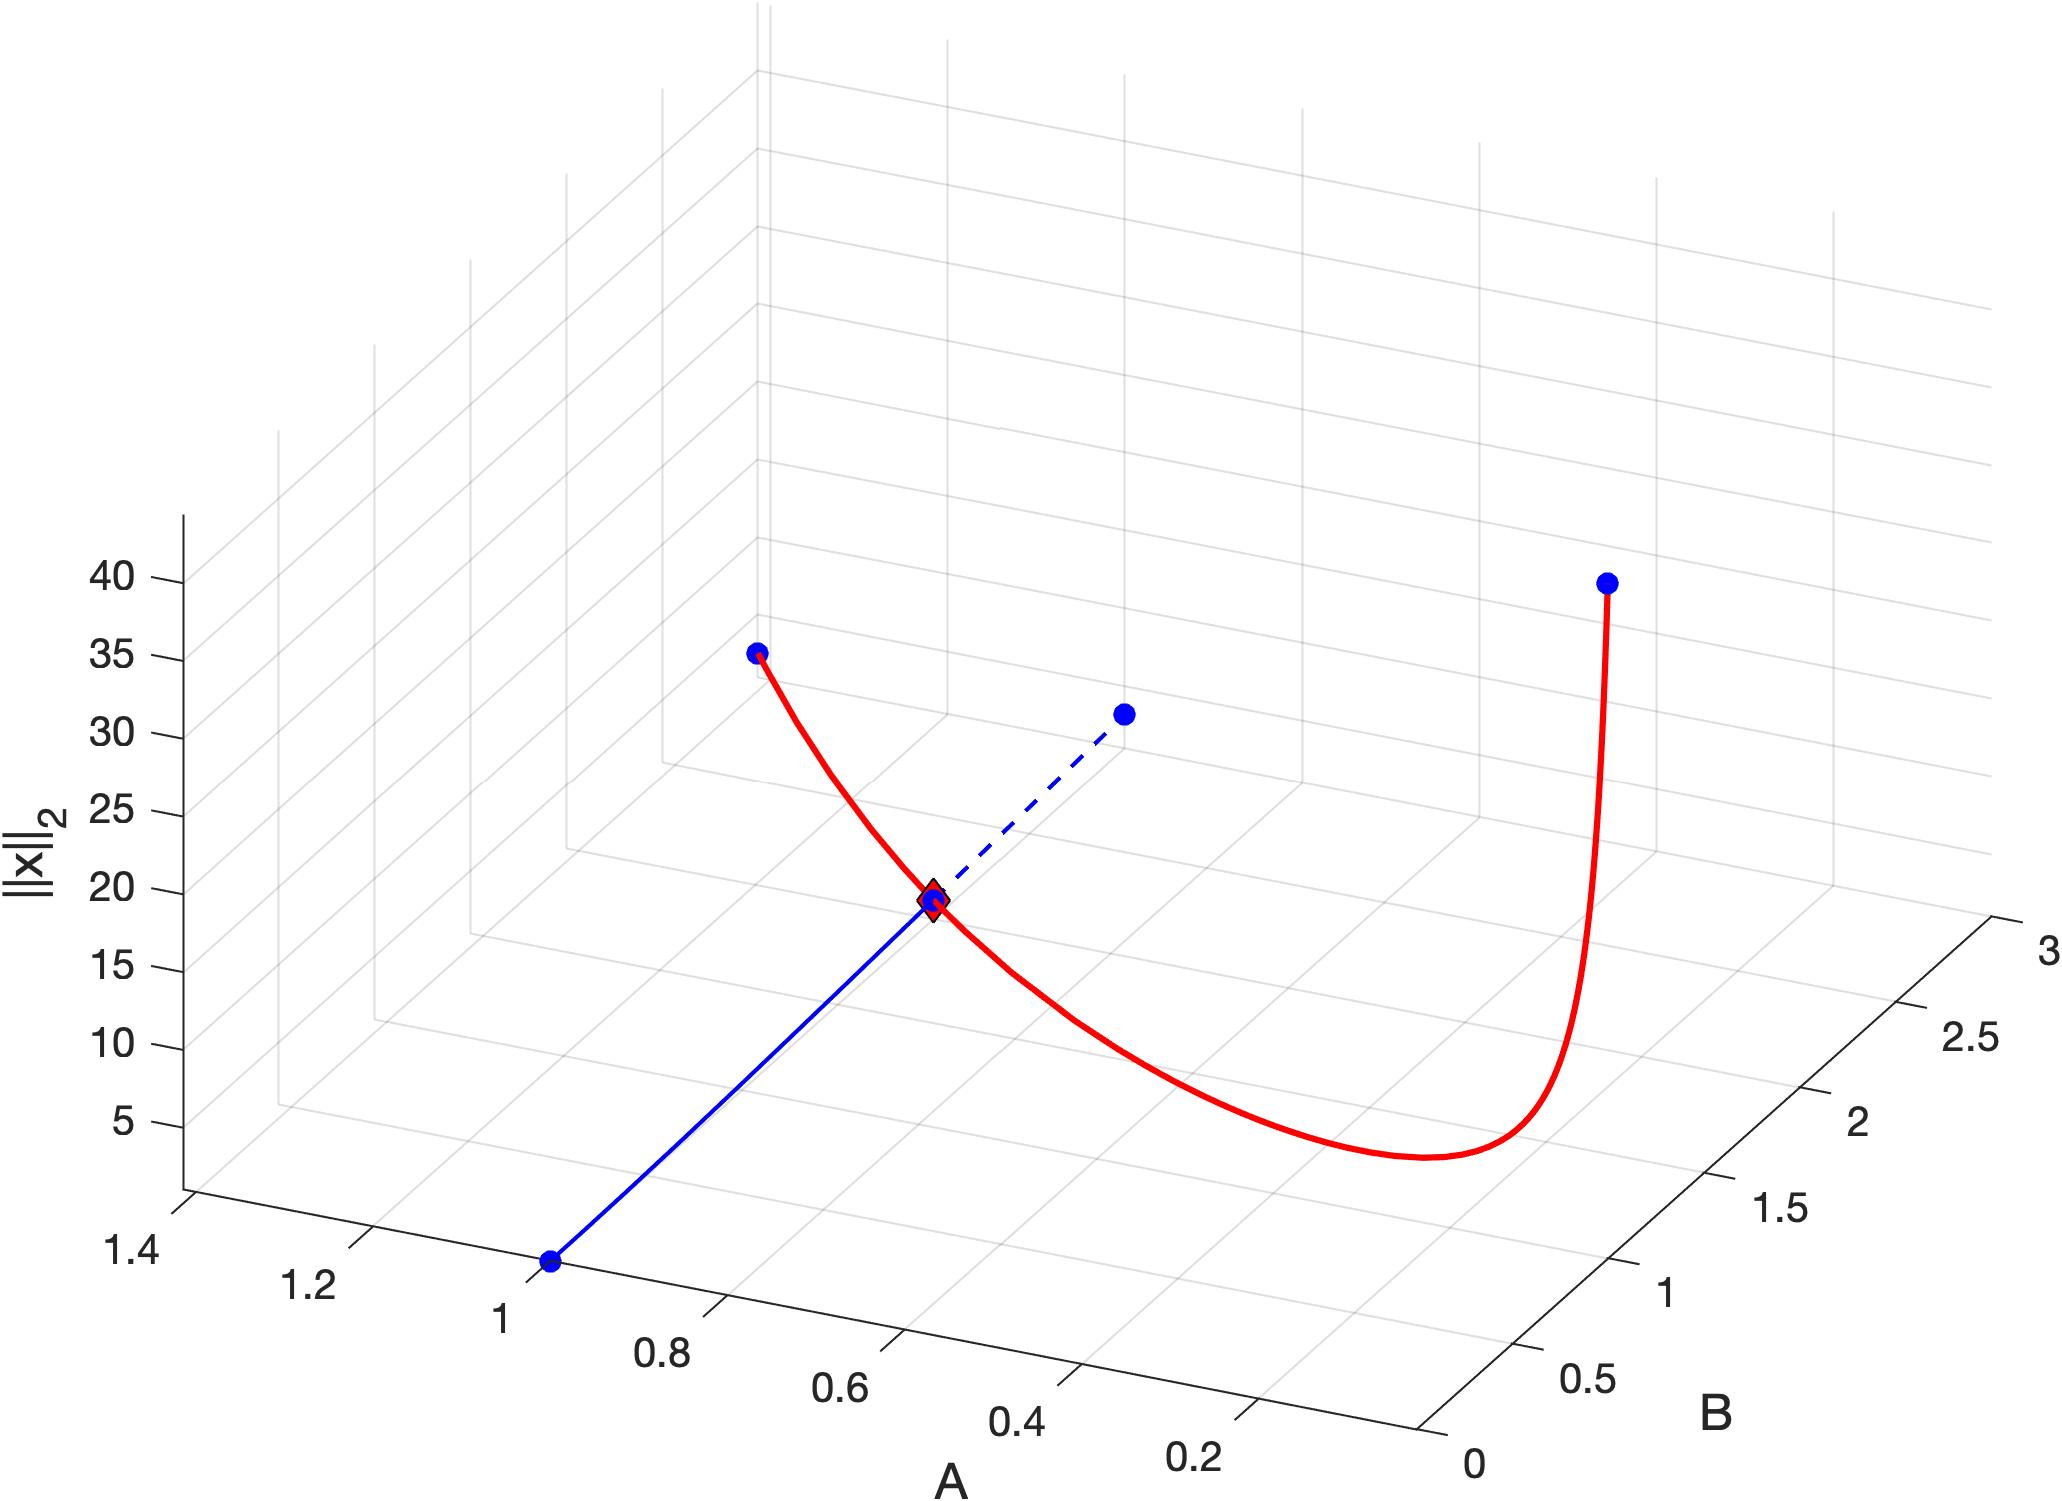
\includegraphics[width=4in]{Figures/Section3_4_1.jpg}
\caption{Bifurcation diagram showing branches of asymptotically stable (blue solid) and unstable (blue dashed) equilibria and Hopf bifurcations (solid red) for the vector field in Section~\ref{sec: Continuing Hopf bifurcations}. The red diamond marks a Hopf bifurcation, while the small blue disks mark the end points of each computation.}
\label{fig: Section3_4_1}
\end{figure}

\subsection{Performing parameter sweeps}
\label{sec: Performing parameter sweeps}
To construct a family of curves of equilibria for discrete values of a second problem parameter, embed the calls to \mcode{coco} and \mcode{coco_plot_bd} in a loop. Consider, for example, the vector field
\[
f(x,p)=\begin{pmatrix}D(1-x_1)e^{x_3}-x_1\\D(1-x_1-\sigma x_2)e^{x_3}-x_2\\BD(1-x_1+\alpha\sigma x_2)e^{x_3}-(1+\beta) x_3\end{pmatrix}
\]
in terms of the vector of state variables $x=(x_1,x_2,x_3)\in\mathbb{R}^3$ and vector of problem parameters $p=(\alpha,\sigma,D,B,\beta)\in\mathbb{R}^5$, and encoded in the function \mcode{abc} shown below.
\begin{lstlisting}[language=coco-highlight,frame=shadowbox]
function f = abc(x,p)

al = p(1,:);
si = p(2,:);
D  = p(3,:);
B  = p(4,:);
be = p(5,:);

x1 = x(1,:);
x2 = x(2,:);
x3 = x(3,:);

e3 = exp(x3);

f(1,:) = D.*(1-x1).*e3-x1;
f(2,:) = D.*(1-x1-si.*x2).*e3-x2;
f(3,:) = D.*B.*(1-x1+al.*si.*x2).*e3-x3.*(1+be);

end
\end{lstlisting}
As in the previous examples, it is possible to derive explicit parameterizations of (five-dimensional) surfaces of equilibria in the $(x_1,x_2,x_3,\alpha,\sigma,D,B,\beta)$ coordinate system and, with greater effort, of four-dimensional surfaces of saddle-node and Hopf bifurcations. As an alternative, for fixed $\alpha$, $\sigma$, $B$, and a sequence of values of $\beta$, the following sequence of commands graphs the corresponding curves of equilibria in a coordinate system with $D$ along the horizontal axis and $\sqrt{x_1^2+x_2^2+x_3^2}$ along the vertical axis (cf.\ Fig.~\ref{fig: Section3_5_1}).
\begin{lstlisting}[language=coco-highlight,frame=lines]
>> clf
>> hold on
>> axis([0.12 0.22 1 7])
>> grid on
>> Nrun = 0;
>> theme = struct('special', {{'SN' 'HB'}});
>> for beta = linspace(1.20, 1.42, 23)
     Nrun = Nrun+1;
     runid = sprintf('run_beta_%d', Nrun);
     coco(runid, 'ode', 'isol', 'ep', @abc, [0; 0; 0], ...
       {'al' 'si' 'D' 'B' 'be'}, [1; 0.04; 0.0; 8; beta], ...
       {'D' 'be'}, [0.0 0.25]);
     coco_plot_bd(theme, runid, 'D', '||x||_2');
   end
\end{lstlisting}
\begin{figure}[h]
\centering
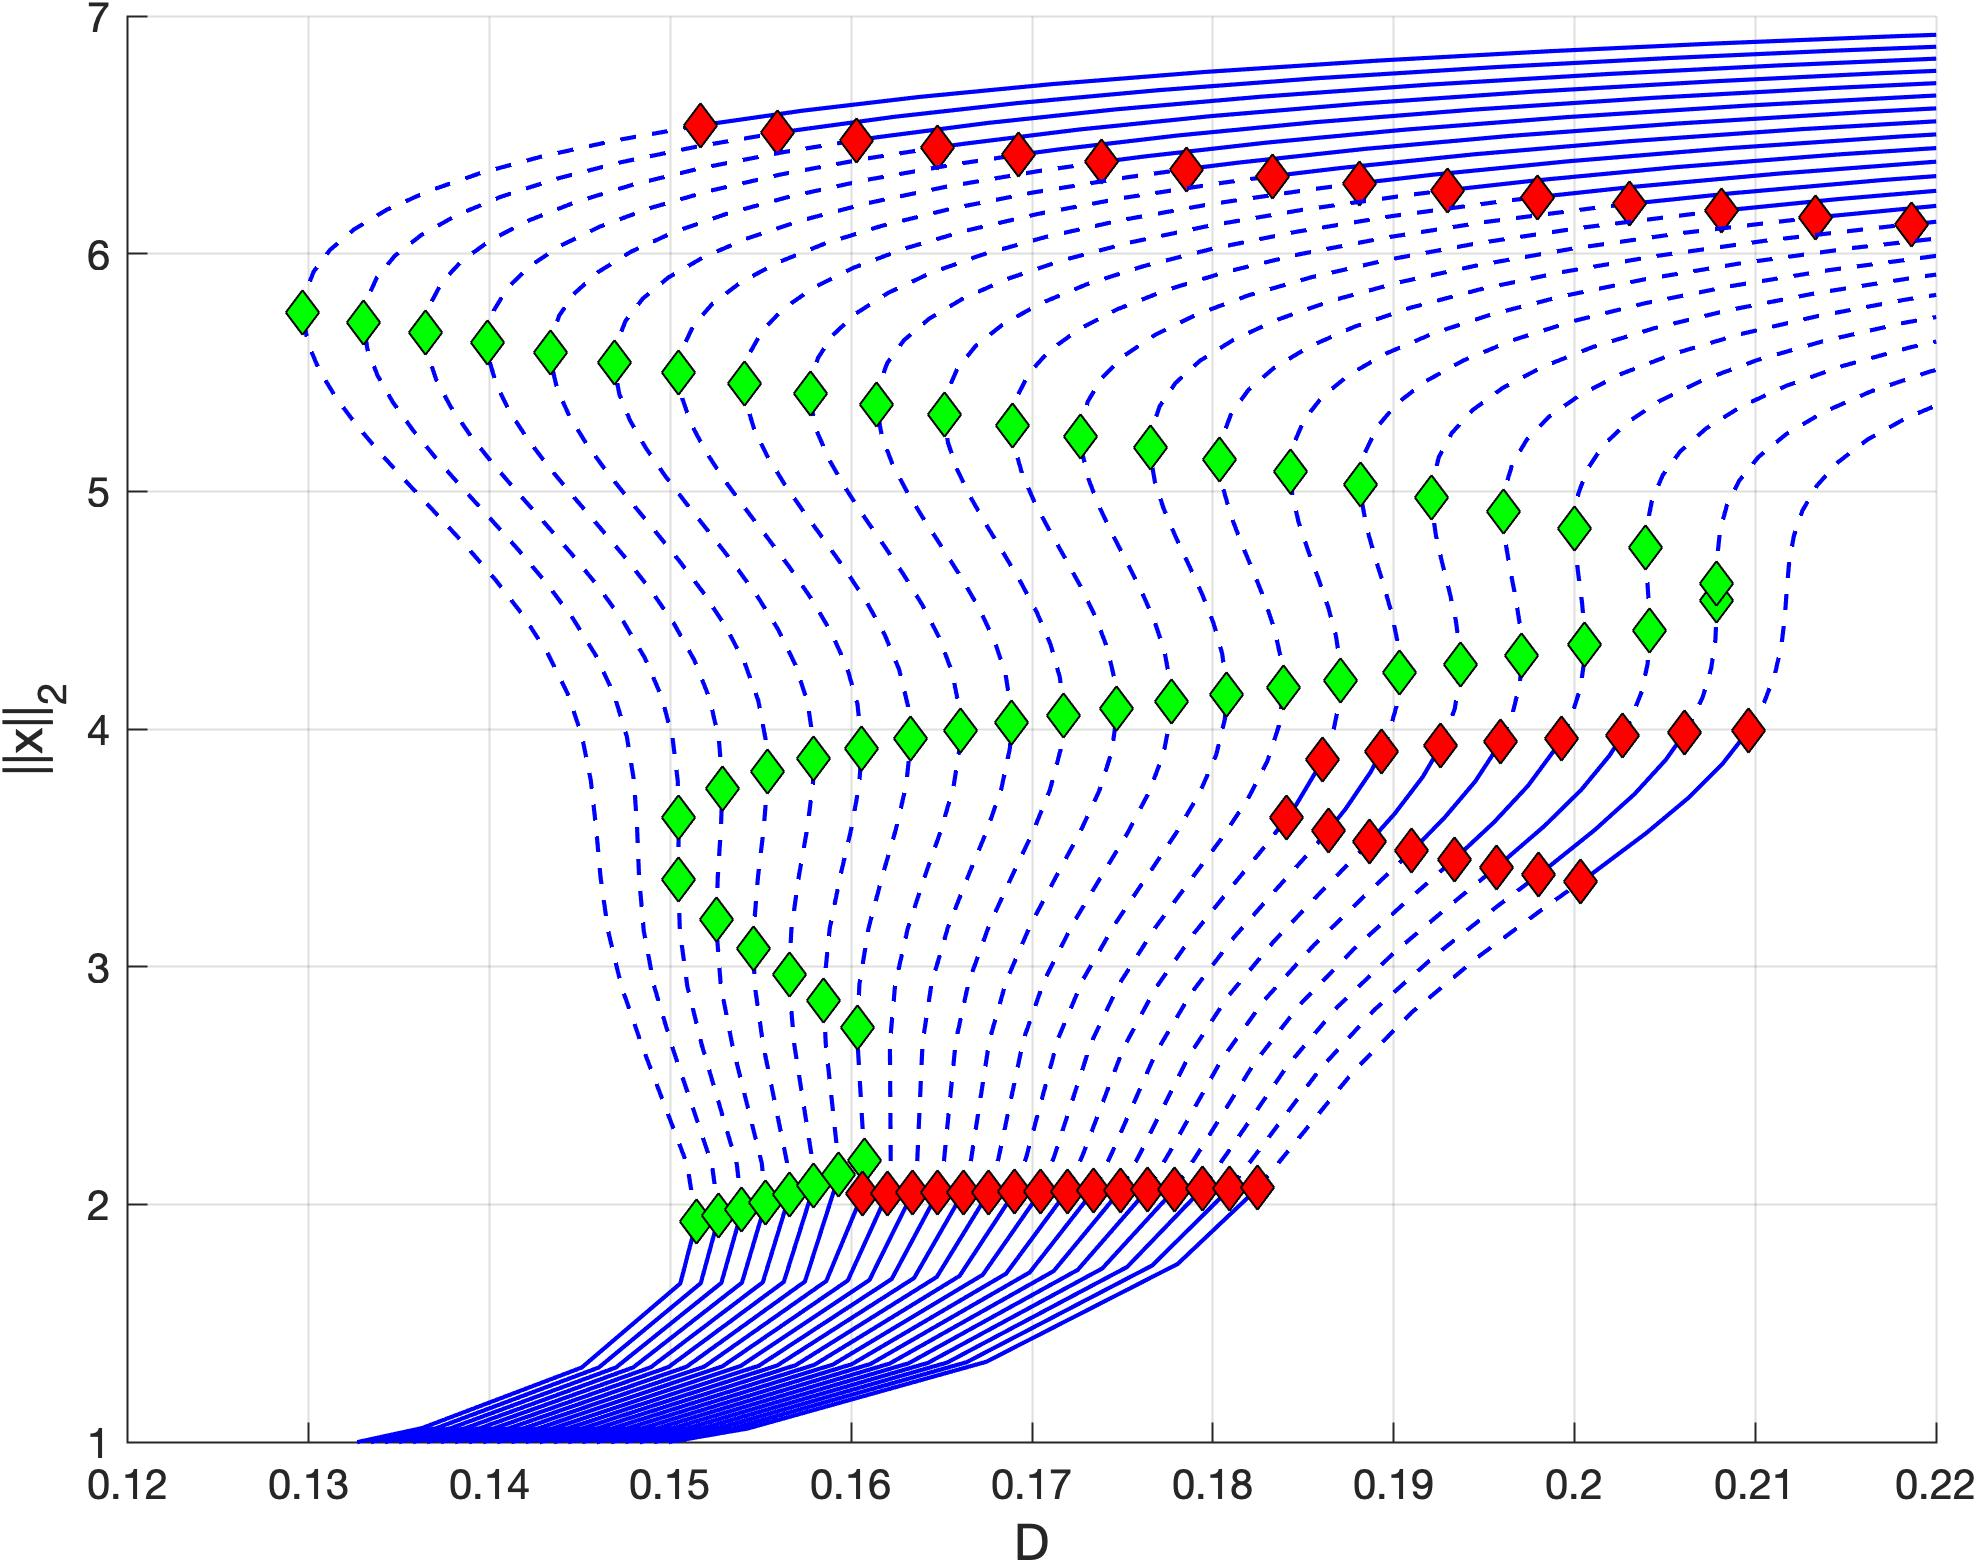
\includegraphics[width=4in]{Figures/Section3_5_1.jpg}
\caption{Bifurcation diagram showing branches of asymptotically stable (blue solid) and unstable (blue dashed) equilibria for the vector field in Section~\ref{sec: Performing parameter sweeps}. The green and red diamonds mark saddle-node and Hopf bifurcations, respectively.}
\label{fig: Section3_5_1}
\end{figure}

Although the screen output is omitted, you will see that the computation signals detection of saddle-node bifurcations and Hopf bifurcations. As expected, it is possible to restart continuation from an \mcode{SN} or \mcode{HB} point in order to compute a family of saddle-node or Hopf bifurcations, respectively. This is accomplished using the commands below.
\begin{lstlisting}[language=coco-highlight,frame=lines]
>> runid = 'run_beta_1';
>> SN = coco_bd_labs(runid, 'SN');
>> coco('run_SN', 'ode', 'SN', 'SN',  ...
     runid, SN(1), {'D' 'be'}, [0.1 0.25]);
>> HB = coco_bd_labs(runid, 'HB');
>> prob = coco_set(coco_prob, 'cont', 'PtMX', 150);
>> coco(prob, 'run_HB', 'ode', 'HB', 'HB', ...
     runid, HB(1), {'D' 'be'}, [0.1 0.8]);
\end{lstlisting}
In the second case, the \mcode{'PtMX'} setting is changed to increases the maximum number of steps that the continuation algorithm takes along each direction of the curve of equilibria to $150$. The resulting curves are then overlaid on top of the diagram generated previously using the following commands (cf.\ Fig.~\ref{fig: Section3_5_2}).
\begin{lstlisting}[language=coco-highlight,frame=lines]
>> theme_SN = struct('special', {{'FP'}});
>> theme_HB = struct('special', {{'FP' 'BTP'}});
>> coco_plot_bd(theme_SN, 'run_SN', 'D', '||x||_2');
>> coco_plot_bd(theme_HB, 'run_HB', 'D', '||x||_2');
>> hold off
\end{lstlisting}
\begin{figure}[h]
\centering
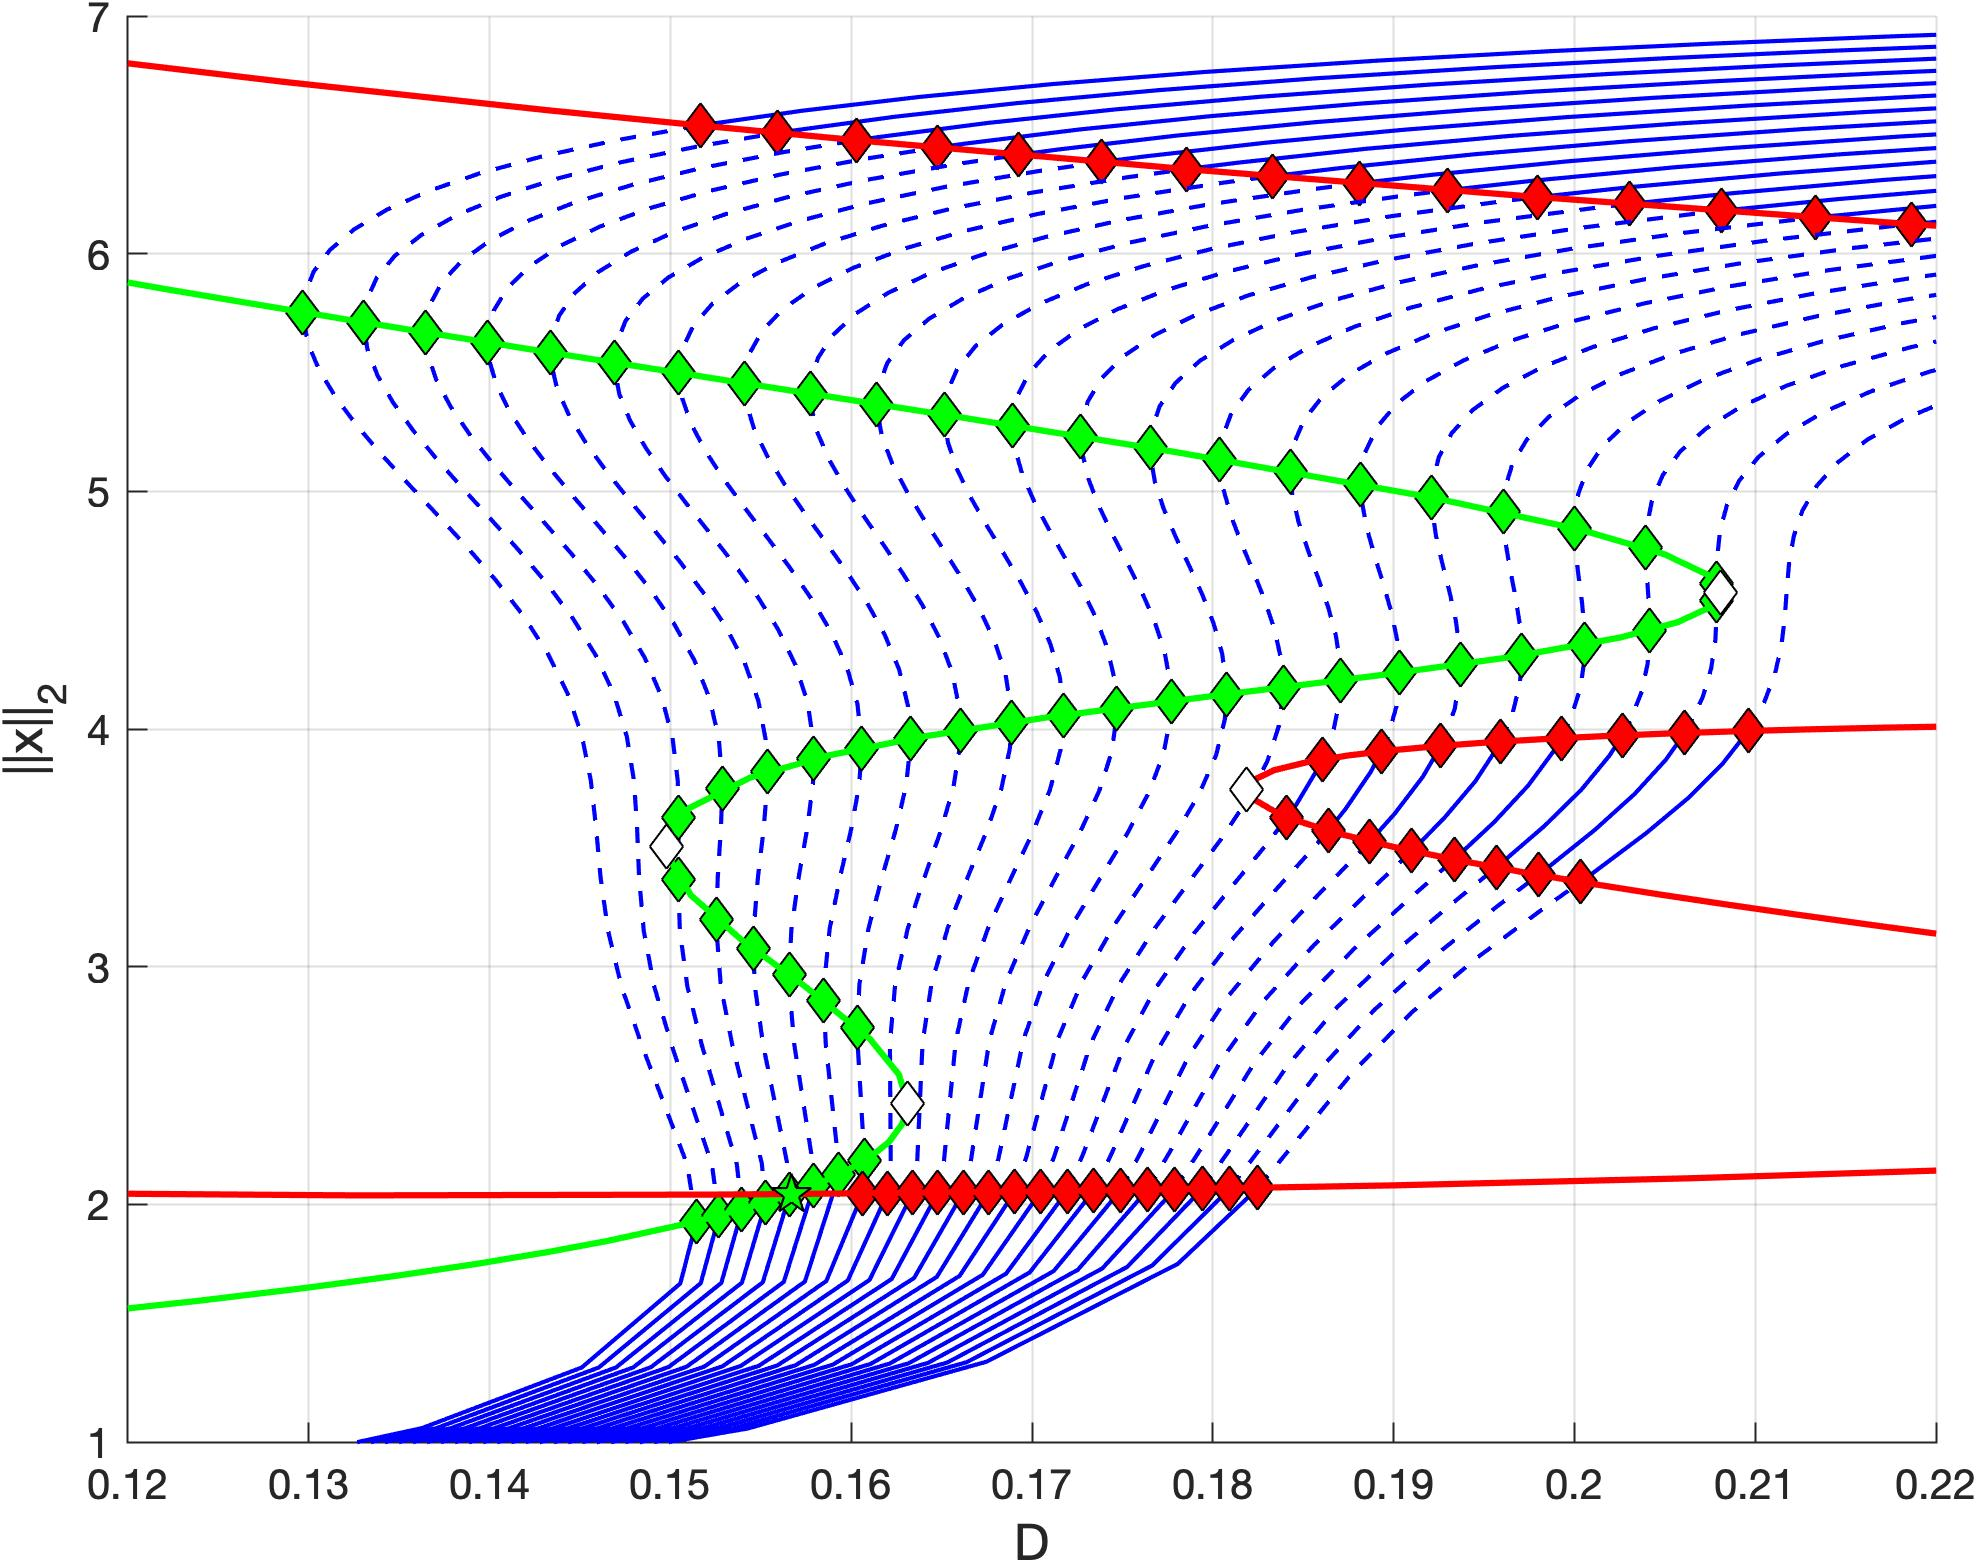
\includegraphics[width=4in]{Figures/Section3_5_2.jpg}
\caption{Bifurcation diagram showing branches of asymptotically stable (blue solid) and unstable (blue dashed) equilibria, saddle-node bifurcations (solid green), and Hopf bifurcations/neutral saddles (red solid) for the vector field in Section~\ref{sec: Performing parameter sweeps}. The green and red diamonds mark saddle-node and Hopf bifurcations, the white diamonds mark fold points, and the green star at the intersection between the curves of saddle-node bifurcations and Hopf bifurcations/neutral saddles marks a Bogdanov-Takens point.}
\label{fig: Section3_5_2}
\end{figure}
The visualization includes a marker highlighting a \textit{Bogdanov-Takens bifurcation} denoted by \mcode{BTP} in the corresponding screen output. Although the algorithm continues past this points, the points to the left of this point are not Hopf bifurcations, but \textit{neutral saddles} that satisfy the algebraic conditions for a Hopf bifurcation, but not the conditions on the eigenvalues of the Jacobian $\partial_xf(x,p)$.

\section{Bifurcations of periodic orbits}
This section demonstrates the use of \textsc{coco} for performing continuation along families of periodic orbits, detecting bifurcations of periodic orbits, performing continuation along families of bifurcation points, and visualizing the results of computation. The calling syntax remains tight, but the examples demonstrate a step up in computational complexity relative to the previous section.

\subsection{Continuing from Hopf bifurcations}
\label{sec: Continuing from Hopf bifurcations}
The pattern of analysis and visualization using \textsc{coco} demonstrated in the previous section also applies to the study of periodic orbits and their bifurcations. 

Consider the following unfolding of the Hopf normal form:
\[
f(x,p)=\begin{pmatrix}-x_2+x_1(p_1+p_2r^2-r^4)\\x_1+x_2(p_1+p_2r^2-r^4)\end{pmatrix},\,r=\sqrt{x_1^2+x_2^2}
\]
in terms of the vector of state variables $x=(x_1,x_2)\in\mathbb{R}^2$ and vector of problem parameters $p=(p_1,p_2)\in\mathbb{R}^2$. Equilibria are found on the two-dimensional surface $x_1=x_2=0$ in the  $(x_1,x_2,p_1,p_2)$ coordinate system and are asymptotically stable for $p_1<0$ and unstable for $p_1>0$. The curve $s\mapsto(0,0,0,s)$ consists of Hopf bifurcation points and coincides with the intersection of the surface of equilibria with the two-dimensional family of periodic orbits $x_1(t)=r^*\cos t$, $x_2(t)=r^*\sin t$, $p_1=r^{*4}-p_2r^{*2}$ for $r^*\ge0$ with nontrivial Floquet multipler $\exp(4\pi r^{*2}(p_2-2r^{*2}))$. It follows that the Hopf bifurcations are \textit{supercritical} for fixed $p_2<0$ and \textit{subcritical} for fixed $p_2>0$. In the latter case, the curve $r^*\mapsto(r^*\cos t,r^*\sin t,-r^{*4},2r^{*2})$ consists of saddle-node bifurcations of periodic orbits, coincident with a curve of folds along the corresponding curves of periodic orbits for fixed $p_2$ and under variations in $p_1$.

The vector field is encoded in the \mcode{hopf} function shown below.
\begin{lstlisting}[language=coco-highlight,frame=shadowbox]
function f = hopf(x,p)

x1 = x(1,:);
x2 = x(2,:);
p1 = p(1,:);
p2 = p(2,:);

r2 = x1.^2+x2.^2;

f(1,:) = x1.*(p1+p2.*r2-r2.^2)-x2;
f(2,:) = x2.*(p1+p2.*r2-r2.^2)+x1;

end
\end{lstlisting}
As a sometimes optional, but mostly required, alternative to a single call to \mcode{coco}, the following demonstrates a separation between problem construction (using the \mcode{ode_isol2ep} constructor) and problem analysis for continuation along a curve of equilibria for $p_2=1$.
\begin{lstlisting}[language=coco-highlight,frame=lines]
>> prob = coco_prob;
>> prob = ode_isol2ep(prob, '', @hopf, [0; 0], {'p1', 'p2'}, [-1; 1]);
>> coco(prob, 'ep_run', [], 'p1', [-1 1]);

    STEP   DAMPING               NORMS              COMPUTATION TIMES
  IT SIT     GAMMA     ||d||     ||f||     ||U||   F(x)  DF(x)  SOLVE
   0                          0.00e+00  1.73e+00    0.0    0.0    0.0

 STEP      TIME        ||U||  LABEL  TYPE            p1
    0  00:00:00   1.7321e+00      1  EP     -1.0000e+00
    5  00:00:00   1.0000e+00      2  HB      1.5899e-07
    8  00:00:00   1.7321e+00      3  EP      1.0000e+00
\end{lstlisting}
The following commands use the constructor \mcode{ode_HB2po} to continue along a curve of periodic orbits emanating from the \mcode{HB} point found in the previous run.
\begin{lstlisting}[language=coco-highlight,frame=lines]
>> HB = coco_bd_labs('ep_run', 'HB');
>> prob = coco_prob;
>> prob = ode_HB2po(prob, '', 'ep_run', HB);
>> coco(prob, 'po_run', [], 'p1', [-1 1]);

    STEP   DAMPING               NORMS              COMPUTATION TIMES
  IT SIT     GAMMA     ||d||     ||f||     ||U||   F(x)  DF(x)  SOLVE
   0                          6.75e-06  8.94e+00    0.0    0.0    0.0
   1   1  1.00e+00  1.96e-06  2.68e-13  8.94e+00    0.0    0.0    0.0
   2   1  1.00e+00  1.14e-12  2.83e-18  8.94e+00    0.0    0.0    0.0

 STEP      TIME        ||U||  LABEL  TYPE            p1
    0  00:00:00   8.9419e+00      1  EP     -9.9933e-07
   10  00:00:00   9.8606e+00      2         -2.2549e-01
   12  00:00:00   1.0251e+01      3  FP     -2.5000e-01
   12  00:00:00   1.0251e+01      4  SN     -2.5000e-01
   20  00:00:00   1.2194e+01      5          4.9782e-01
   23  00:00:01   1.2762e+01      6  EP      1.0000e+00

 STEP      TIME        ||U||  LABEL  TYPE            p1
    0  00:00:01   8.9419e+00      7  EP     -9.9933e-07
    1  00:00:01   8.9419e+00      8  FP     -1.7508e-10
    2  00:00:01   8.9423e+00      9  BP     -1.7270e-04
   10  00:00:01   9.8546e+00     10         -2.2476e-01
   12  00:00:01   1.0251e+01     11  FP     -2.5000e-01
   12  00:00:01   1.0251e+01     12  SN     -2.5000e-01
   20  00:00:02   1.2188e+01     13          4.9312e-01
   23  00:00:02   1.2762e+01     14  EP      1.0000e+00
\end{lstlisting}
The screen output includes three labeled points of type \mcode{FP}, two of type \mcode{SN}, and one of type \mcode{BP}. Of these, the first and third \mcode{FP} points denote folds along the curve of periodic orbits, which coincide with (cyclic) saddle-node bifurcations. The second \mcode{FP} point and the single \mcode{BP} point coincide approximately with the Hopf bifurcation, which is detected as both a branch point of periodic orbits and a fold along this curve.

The curve of saddle-node bifurcations of periodic orbits that runs through the first \mcode{SN} point found above can be computed using the \mcode{ode_po2SN} constructor as shown next.
\begin{lstlisting}[language=coco-highlight,frame=lines]
>> SN = coco_bd_labs('po_run', 'SN');
>> prob = coco_prob;
>> prob = ode_po2SN(prob, '', 'po_run', SN(1));
>> coco(prob, 'po_SN_run', [], {'p1', 'p2'}, {[-1 1] [0.001 3]});

    STEP   DAMPING               NORMS              COMPUTATION TIMES
  IT SIT     GAMMA     ||d||     ||f||     ||U||   F(x)  DF(x)  SOLVE
   0                          1.21e-05  1.25e+01    0.0    0.0    0.0
   1   1  1.00e+00  4.97e-05  7.60e-09  1.25e+01    0.0    0.0    0.0
   2   1  1.00e+00  1.70e-08  3.56e-09  1.25e+01    0.0    0.0    0.0

 STEP      TIME        ||U||  LABEL  TYPE            p1           p2
    0  00:00:00   1.2493e+01      1  EP     -2.5000e-01   1.0000e+00
    8  00:00:00   1.3746e+01      2  EP     -1.0000e+00   2.0000e+00

 STEP      TIME        ||U||  LABEL  TYPE            p1           p2
    0  00:00:00   1.2493e+01      3  EP     -2.5000e-01   1.0000e+00
   10  00:00:00   1.1412e+01      4         -6.3961e-04   5.0581e-02
   12  00:00:00   1.1357e+01      5  EP     -2.5000e-07   1.0000e-03
\end{lstlisting}
The computational domain excludes $p_2=0$ to avoid redundant covering of the curve. 

Finally, the following commands rely on the \mcode{ode_ep2HB} constructor to perform continuation along the curve of Hopf bifurcations with detection of special points at designated values of $p_2$.
\begin{lstlisting}[language=coco-highlight,frame=lines]
>> prob = coco_prob;
>> prob = ode_ep2HB(prob, '', 'ep_run', HB);
>> prob = coco_add_event(prob, 'UZ', 'p2', setdiff(-2:0.5:3,1));
>> coco(prob, 'ep_HB_run', [], {'p1' 'p2'}, {[-1 1] [-2.01 3.01]});

    STEP   DAMPING               NORMS              COMPUTATION TIMES
  IT SIT     GAMMA     ||d||     ||f||     ||U||   F(x)  DF(x)  SOLVE
   0                          2.25e-07  2.65e+00    0.0    0.0    0.0

 STEP      TIME        ||U||  LABEL  TYPE            p1           p2
    0  00:00:00   2.6458e+00      1  EP      1.5899e-07   1.0000e+00
    4  00:00:00   3.0822e+00      2  UZ      1.5399e-07   1.5000e+00
    5  00:00:00   3.6056e+00      3  UZ      1.4899e-07   2.0000e+00
    6  00:00:00   4.1833e+00      4  UZ      1.4399e-07   2.5000e+00
    8  00:00:00   4.7958e+00      5  UZ      1.3899e-07   3.0000e+00
    8  00:00:00   4.8083e+00      6  EP      1.3889e-07   3.0100e+00

 STEP      TIME        ||U||  LABEL  TYPE            p1           p2
    0  00:00:00   2.6458e+00      7  EP      1.5899e-07   1.0000e+00
    4  00:00:00   2.3452e+00      8  UZ      1.6399e-07   5.0000e-01
    5  00:00:00   2.2361e+00      9  UZ      1.6899e-07  -2.7756e-17
    6  00:00:00   2.3452e+00     10  UZ      1.7399e-07  -5.0000e-01
    8  00:00:00   2.6458e+00     11  UZ      1.7899e-07  -1.0000e+00
    9  00:00:00   3.0822e+00     12  UZ      1.8399e-07  -1.5000e+00
   10  00:00:00   3.5341e+00     13          1.8834e-07  -1.9352e+00
   11  00:00:00   3.6056e+00     14  UZ      1.8899e-07  -2.0000e+00
   11  00:00:00   3.6167e+00     15  EP      1.8909e-07  -2.0100e+00
\end{lstlisting}
Each such special point is the basis for a separate continuation run along a curve of periodic orbits using the commands shown below.
\begin{lstlisting}[language=coco-highlight,frame=lines]
>> labs = coco_bd_labs('ep_HB_run', 'UZ');
>> for lab=labs
     runid = sprintf('po%d_run', lab);
     prob = coco_prob;
     prob = ode_HB2po(prob, '', 'ep_HB_run', lab);
     coco(prob, runid, [], {'p1' 'p2'}, [-1.01 1]);
   end
\end{lstlisting}
The following sequence of commands visualizes the results of these computations (cf.\ Fig.~\ref{fig: Section4_1_1}).
\begin{lstlisting}[language=coco-highlight,frame=lines]
>> clf; hold on; grid on; box on
>> axis([-1.5 1 -2 4 0 1.6]); view(3)
>> thm = struct('zlab', '||x||_2');
>> thm.special = {'EP', 'HB'};
>> coco_plot_bd(thm, 'ep_run', 'p1', 'p2', '||x||_2')
>> thm.special =  {'EP', 'SN'};
>> coco_plot_bd(thm, 'po_run', 'p1', 'p2', '||x||_{2,MPD}')
>> thm.special = {};
>> coco_plot_bd(thm, 'po_SN_run', 'p1', 'p2', '||x||_{2,MPD}')
>> thm.special = {};
>> coco_plot_bd(thm, 'ep_HB_run', 'p1', 'p2', '||x||_2')
>> thm.special = {'EP'}
>> for lab=labs
     runid = sprintf('po%d_run', lab);
     coco_plot_bd(thm, runid, 'p1', 'p2', '||x||_{2,MPD}')
   end
>> hold off
\end{lstlisting}
\begin{figure}[h]
\centering
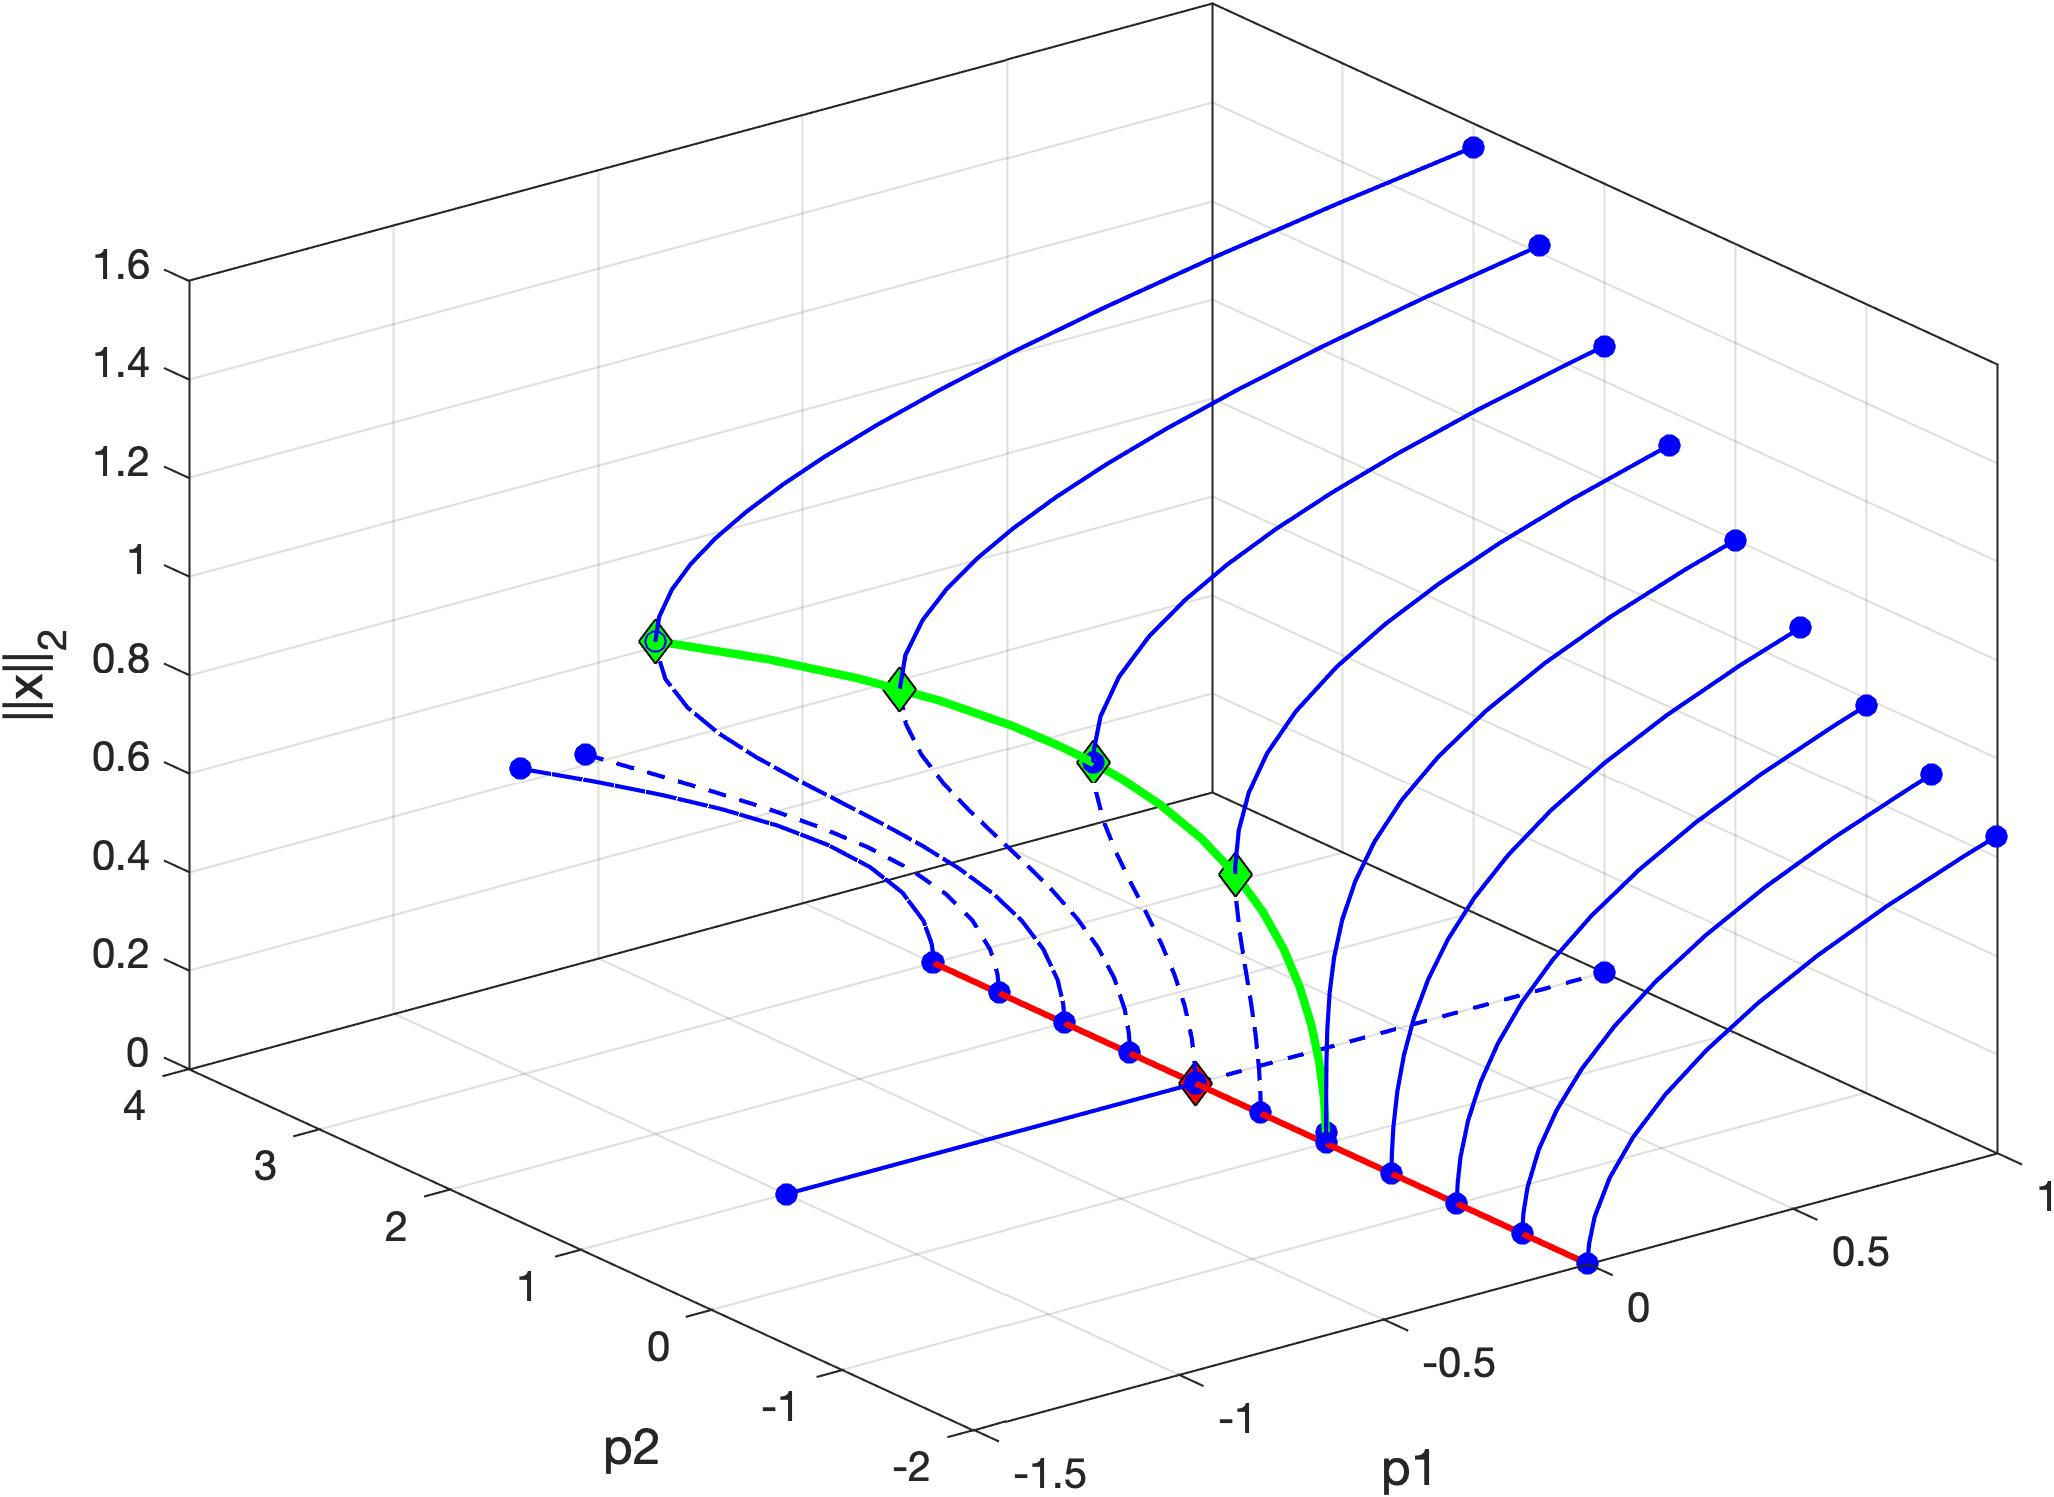
\includegraphics[width=4in]{Figures/Section4_1_1.jpg}
\caption{Bifurcation diagram showing branches of asymptotically stable (blue solid) and unstable (blue dashed) equilibria and periodic orbits, saddle-node bifurcations of periodic orbits (solid green), and Hopf bifurcations (red solid) for the vector field in Section~\ref{sec: Continuing from Hopf bifurcations}. The green and red diamonds mark saddle-node and Hopf bifurcations, and the blue disks mark the end points of each computation.}
\label{fig: Section4_1_1}
\end{figure}
Here, the vertical axis represents the Euclidean norm $\|x\|_2$ for the equilibria and a suitably defined scalar magnitude for the periodic orbits.

\subsection{Finding isolated curves and branch points}
\label{sec: Finding isolated curves}
As needed, the default pseudo-arclength continuation algorithm used by \textsc{coco} relies on finite-difference approximations for derivatives of the vector field with respect to $x$ and $p$. When exact derivatives are available, these may provided to \textsc{coco} in order to eliminate a source of approximation errors, especially during continuation of bifurcations. As an example, the following functions encode the vector field in Section~\ref{sec: Performing parameter sweeps} and its first derivatives with respect to $x$ and $p$.
\begin{lstlisting}[language=coco-highlight,frame=shadowbox]
function f = abc(x,p)

al = p(1,:);
si = p(2,:);
D  = p(3,:);
B  = p(4,:);
be = p(5,:);

x1 = x(1,:);
x2 = x(2,:);
x3 = x(3,:);

e3 = exp(x3);

f(1,:) = D.*(1-x1).*e3-x1;
f(2,:) = D.*(1-x1-si.*x2).*e3-x2;
f(3,:) = D.*B.*(1-x1+al.*si.*x2).*e3-x3.*(1+be);

end
\end{lstlisting}
\begin{lstlisting}[language=coco-highlight,frame=shadowbox]
function J = abc_dx(x,p)

al = p(1,:);
si = p(2,:);
D  = p(3,:);
B  = p(4,:);
be = p(5,:);

x1 = x(1,:);
x2 = x(2,:);
x3 = x(3,:);

e3 = exp(x3);

J = zeros(3,3,numel(e3));
J(1,1,:) = -1-D.*e3;
J(1,3,:) = D.*(1-x1).*e3;
J(2,1,:) = -D.*e3;
J(2,2,:) = -1-D.*si.*e3;
J(2,3,:) = D.*(1-x1-si.*x2).*e3;
J(3,1,:) = -D.*B.*e3;
J(3,2,:) = D.*B.*al.*si.*e3;
J(3,3,:) = -1-be+D.*B.*(1-x1+al.*si.*x2).*e3;

end
\end{lstlisting}
\begin{lstlisting}[language=coco-highlight,frame=shadowbox]
function J = abc_dp(x,p)

al = p(1,:);
si = p(2,:);
D  = p(3,:);
B  = p(4,:);

x1 = x(1,:);
x2 = x(2,:);
x3 = x(3,:);

e3 = exp(x3);

J = zeros(3,5,numel(e3));
J(1,3,:) = (1-x1).*e3;
J(2,2,:) = -D.*x2.*e3;
J(2,3,:) = (1-x1-si.*x2).*e3;
J(3,1,:) = D.*B.*si.*x2.*e3;
J(3,2,:) = D.*B.*al.*x2.*e3;
J(3,3,:) = B.*(1-x1+al.*si.*x2).*e3;
J(3,4,:) = D.*(1-x1+al.*si.*x2).*e3;
J(3,5,:) = -x3;

end
\end{lstlisting}
%A \textsc{coco} interface to the symbolic toolbox in \textsc{Matlab} can be used to generate functions that evaluate the exact derivatives to desired order. As an example, the following commands assign function handles to the vector field in Section~\ref{sec: Performing parameter sweeps} and its derivatives with respect to $x$ and $p$ to the cell array \mcode{funcs}.
%\begin{lstlisting}[language=coco-highlight,frame=lines]
%>> syms x1 x2 x3 al si D B be
%>> f = [D*(1-x1)*exp(x3)-x1; 
%     D*(1-x1-si*x2)*exp(x3)-x2; 
%     B*D*(1-x1+al*si*x2)*exp(x3)-(1+be)*x3];
%>> F = sco_sym2funcs(f, {[x1; x2; x3], [al; si; D; B; be]}, ...
%     {'x', 'p'}, 'filename', 'sys_abc');
%>> funcs = {F(''), F('x'), F('p')};
%\end{lstlisting}
The following then computes branches of equilbria and periodic orbits emanating from Hopf bifurcations for four different values of the $\beta$ parameter.
\begin{lstlisting}[language=coco-highlight,frame=lines]
>> PtMX = [255 90; 260 100; 240 100; 70 100];
>> beta = 1.55:0.01:1.58;
>> for i=1:4
     eprunid = sprintf('run_ep%d', i);
     coco(eprunid, 'ode', 'isol', 'ep', @abc, @abc_dx, @abc_dp, [0; 0; 0], ...
       {'al' 'si' 'D' 'B' 'be'}, [1; 0.04; 0; 8; beta(i)], ...
       'D', [0 0.4]);
  
     HB = coco_bd_labs(eprunid, 'HB');
     prob = coco_prob;
     porunid = sprintf('run_po1%d', i);
     prob = coco_set(prob, 'cont', 'NAdapt', 1, 'PtMX', [0 PtMX(i,1)]);
     coco(prob, porunid, 'ode', 'HB', 'po', eprunid, HB(1), ...
       'D', [0 0.4]);
       
     prob = coco_prob;
     prob = coco_set(prob, 'cont', 'NAdapt', 1, 'PtMX', [0 PtMX(i,2)]);
     porunid = sprintf('run_po2%d', i);
     coco(prob, porunid, 'ode', 'HB', 'po', eprunid, HB(3), ...
       'D', [0 0.4]);
   end
\end{lstlisting}
The \mcode{'NAdapt'} setting of $1$ ensures that the discretization used to approximate the periodic orbits is updated before each step of the continuation algorithm to manage growth of the truncation error. The values for the \mcode{'PtMX'} setting are chosen (a posteriori) to avoid redundant covering of the curves of periodic orbits. The results of the computation are visualized as follows (cf.\ Fig.~\ref{fig: Section4_2_1}).
\begin{lstlisting}[language=coco-highlight,frame=lines]
>> clf
>> theme_ep = struct();
>> theme_ep.special = {'HB'};
>> theme_po = struct();
>> theme_po.lspec = {{'k-', 'LineWidth', 1}, {'k--', 'LineWidth', 1}};
>> theme_po.special = {'SN'};
>> for i=1:4
     subplot(2,2,i)
     axis([0.15 0.4 1 10])
     grid on
     hold on
     eprunid = sprintf('run_ep%d', i);
     coco_plot_bd(theme_ep, eprunid, 'D', 'MAX(x)', 3);

     porunid = sprintf('run_po1%d', i);
     coco_plot_bd(theme_po, porunid, 'D', 'MAX(x)', 3)
  
     porunid = sprintf('run_po2%d', i);
     coco_plot_bd(theme_po, porunid, 'D', 'MAX(x)', 3);
     hold off
   end
\end{lstlisting}
\begin{figure}[h]
\centering
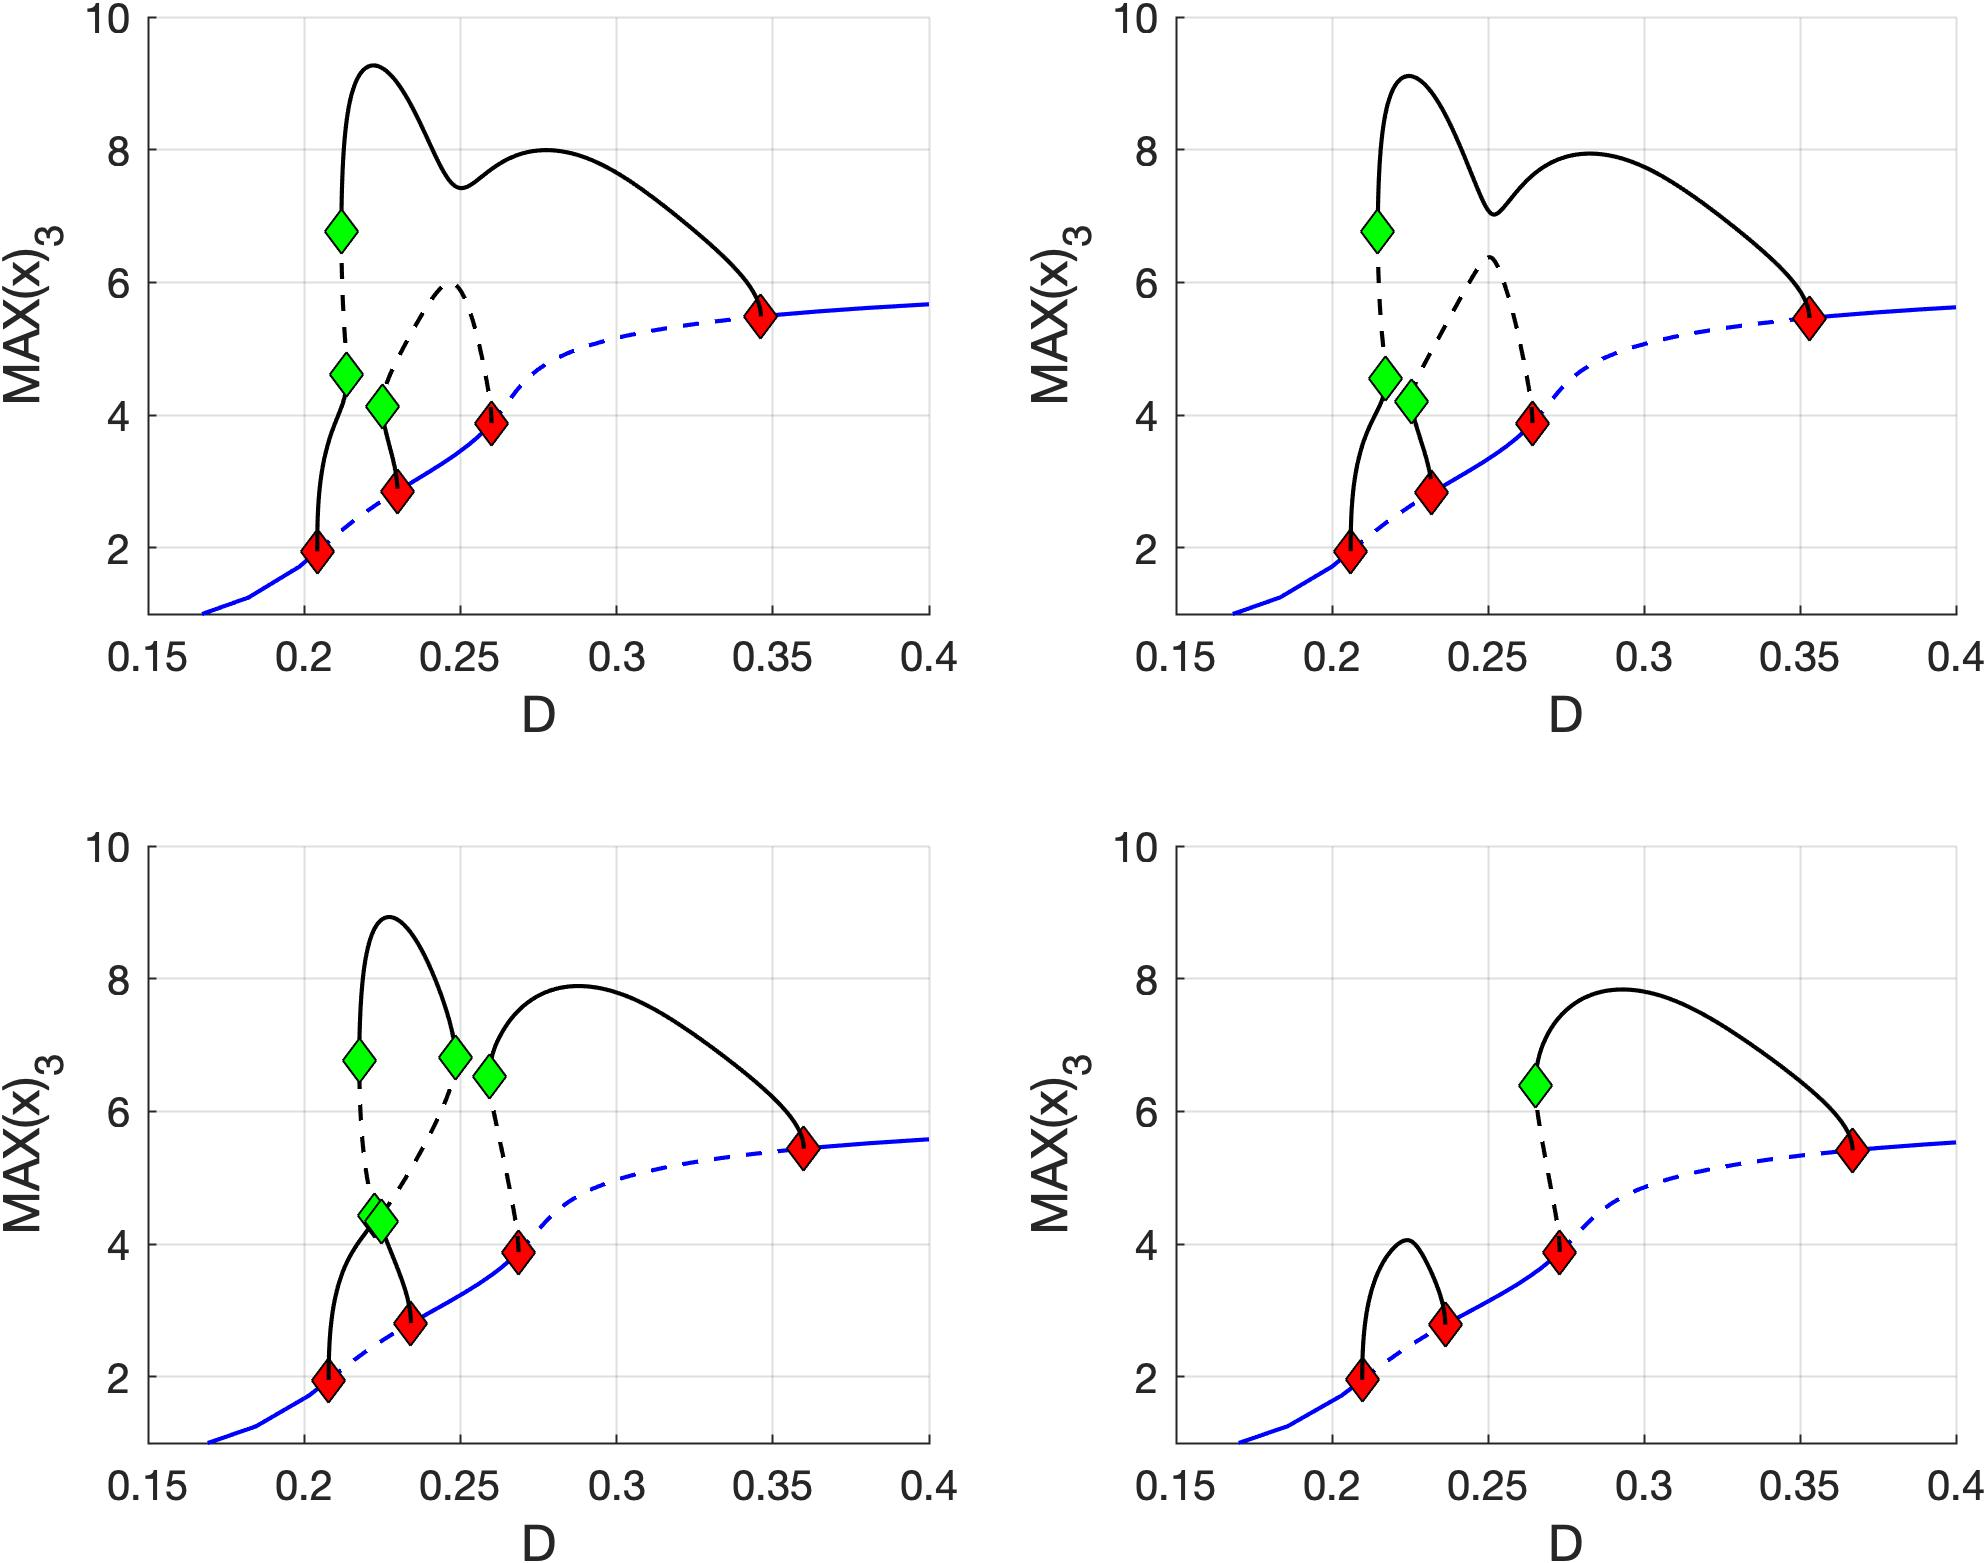
\includegraphics[width=4in]{Figures/Section4_2_1.jpg}
\caption{Bifurcation diagram showing branches of asymptotically stable (blue solid) and unstable (blue dashed) equilibria, as well as asymptotically stable (black solid) and unstable (black dashed) periodic orbits for the vector field in Section~\ref{sec: Finding isolated curves}. The green and red diamonds mark saddle-node and Hopf bifurcations.}
\label{fig: Section4_2_1}
\end{figure}

The change in organization of the branches of periodic orbits between the bottom two panels suggest the appearance of an isolated closed curve of periodic orbits in the bottom right panel that has pinched off from the main branch at a branch point for some value of $\beta$ between $1.57$ and $1.58$. This curve is computed by first continuing from a periodic orbit found in the bottom left panel (label 15 in the corresponding computation) under variations in $\beta$, and then holding $\beta$ fixed and again varying $D$ as shown below.
\begin{lstlisting}[language=coco-highlight,frame=lines]
>> prob = coco_prob;
>> prob = coco_set(prob, 'cont', 'NAdapt', 1, 'PtMX', [0 200]);
>> porunid = 'run_po3';
>> coco(prob, porunid, 'ode', 'po', 'po', 'run_po13', 15, ...
     'be', [beta(3) beta(4)]);
>> prob = coco_prob;
>> prob = coco_set(prob, 'cont', 'NAdapt', 1, 'PtMX', [0 160]);
>> porunid = 'run_po34';
>> coco(prob, porunid, 'ode', 'po', 'po', 'run_po3', 3, ...
     'D', [0 0.4]);
\end{lstlisting}
The isolated curve is made visible in the bifurcation diagram as follows (cf.\ Fig.~\ref{fig: Section4_2_2}).
\begin{lstlisting}[language=coco-highlight,frame=lines]
>> hold on
>> coco_plot_bd(theme_po,  'run_po34', 'D', 'MAX(x)', 3);
>> hold off
\end{lstlisting}
\begin{figure}[h]
\centering
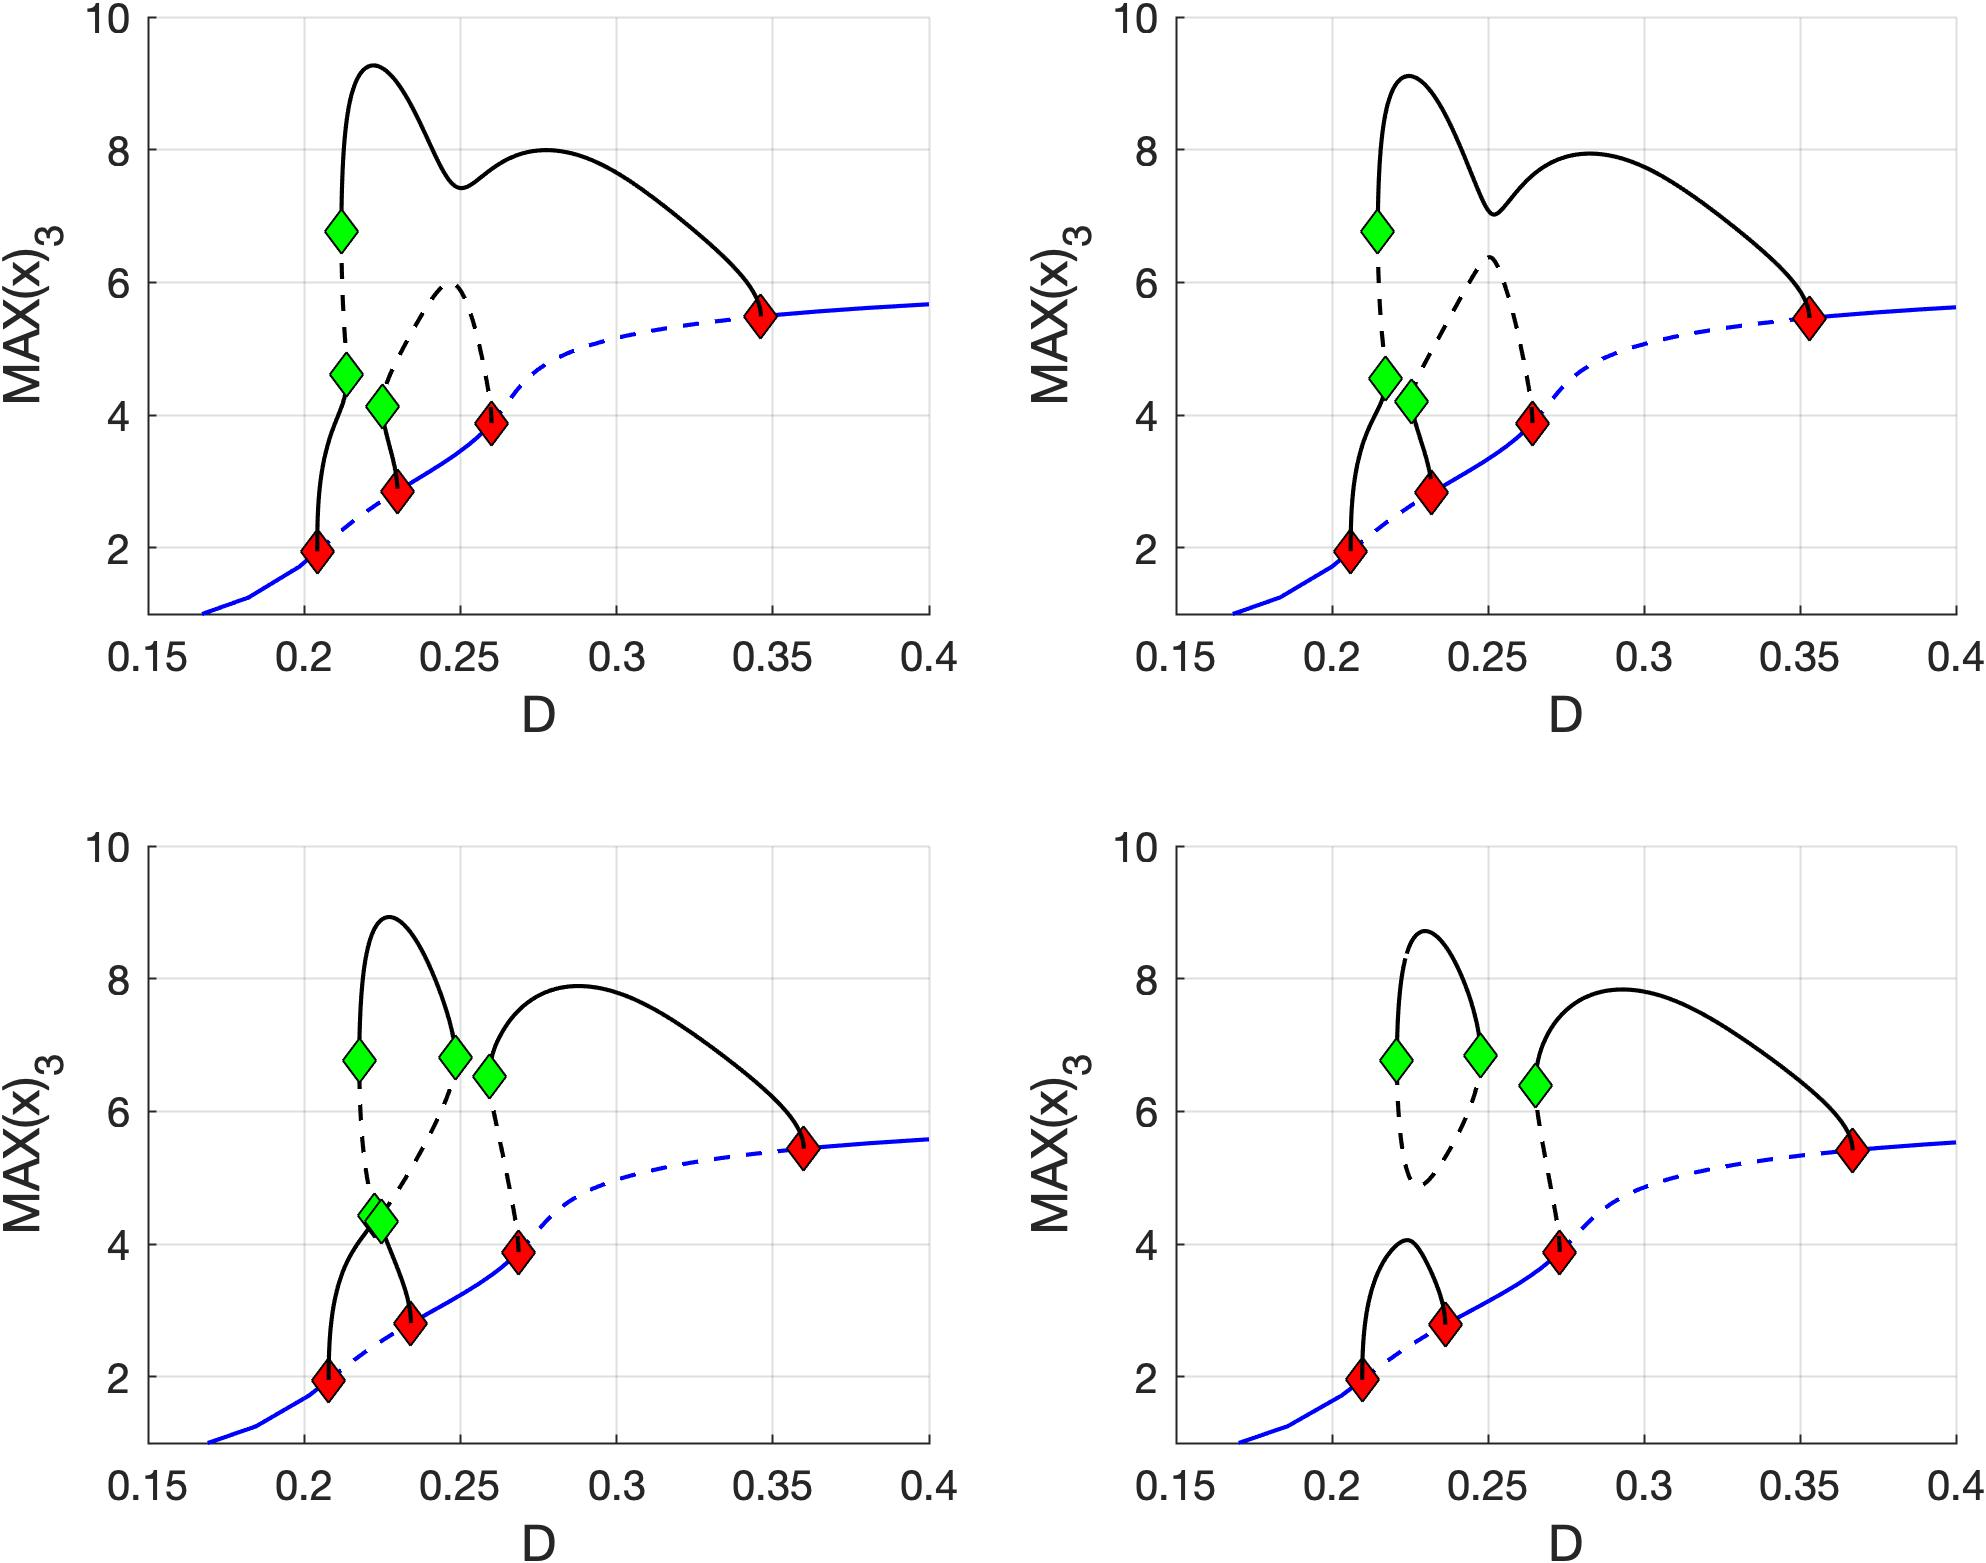
\includegraphics[width=4in]{Figures/Section4_2_2.jpg}
\caption{Bifurcation diagram showing branches of asymptotically stable (blue solid) and unstable (blue dashed) equilibria, as well as asymptotically stable (black solid) and unstable (black dashed) periodic orbits for the vector field in Section~\ref{sec: Finding isolated curves}. The green and red diamonds mark saddle-node and Hopf bifurcations. The diagram differs from that in Fig.~\ref{fig: Section4_2_1} by the inclusion of the isolated curve of periodic orbits in the bottom right panel.}
\label{fig: Section4_2_2}
\end{figure}

The values of $\beta$ and $D$ where the isolated curve pinches off from the main branch corresponds to a fold point along the curve of saddle-node bifurcations of periodic orbits found using the following commands.
\begin{lstlisting}[language=coco-highlight,frame=lines]
>> porunid = 'run_po11';
>> prob = coco_prob;
>> prob = coco_set(prob, 'cont', 'NAdapt', 1, 'PtMX', [0 100], 'h_max', 5);
>> SN = coco_bd_labs(porunid, 'SN');
>> coco(prob, 'po_run_SN', 'ode', 'SN', 'SN', ...
     porunid, SN(1), {'be', 'D'}, {[1.55 1.58], [0 0.4]});
     
    STEP   DAMPING               NORMS              COMPUTATION TIMES
  IT SIT     GAMMA     ||d||     ||f||     ||U||   F(x)  DF(x)  SOLVE
   0                          3.67e-06  1.68e+02    0.0    0.0    0.0
   1   1  1.00e+00  6.90e-04  1.89e-09  1.68e+02    0.0    0.0    0.0
   2   1  1.00e+00  1.25e-08  1.83e-13  1.68e+02    0.0    0.0    0.0

 STEP      TIME        ||U||  LABEL  TYPE            be            D
    0  00:00:00   1.6753e+02      1  EP      1.5500e+00   2.1370e-01
   10  00:00:01   1.8824e+02      2          1.5534e+00   2.1481e-01
   20  00:00:02   2.3148e+02      3          1.5603e+00   2.1735e-01
   30  00:00:03   2.7568e+02      4          1.5676e+00   2.2070e-01
   37  00:00:04   3.0056e+02      5  FP      1.5706e+00   2.2365e-01
   40  00:00:05   3.0825e+02      6          1.5694e+00   2.2488e-01
   50  00:00:06   3.0765e+02      7          1.5574e+00   2.2552e-01
   54  00:00:07   3.0433e+02      8  EP      1.5500e+00   2.2496e-01
\end{lstlisting}


\subsection{A web of bifurcations}
\label{sec: A web of bifurcations}
Analogously to the detection and continuation of saddle-node bifurcations of periodic orbits, it is straightforward to detect and continue \textit{period-doubling} and \textit{Neimark-Sacker/torus bifurcations} using \textsc{coco}. 

Consider the autonomous dynamical system given by the vector field
\[
f(x,p)=\left(\begin{array}{c}( -(\beta+\nu)x_1+\beta x_2  - A_3x_1^3 + B_3(x_2-x_1)^3 )/r\\
\beta x_1 - (\beta+\gamma)x_2 - x_3 - B_3(x_2-x_1)^3\\x_2\end{array}\right)
\]
in terms of the vector of state variables $x=(x_1,x_2,x_3)\in\mathbb{R}^3$ and the vector of problem parameters $p=(\nu,\beta,\gamma,r,A_3,B_3)\in\mathbb{R}^6$. In addition to the equilibrium at the origin, there exist two families of equilibria located at
\[
(x_1,x_2,x_3)=\left(\pm\frac{\sqrt{-\beta-\nu}}{\sqrt{A_3+B_3}},0,\pm\frac{\sqrt{-\beta-\nu}}{\sqrt{A_3+B_3}}\frac{A_3\beta-B_3\mu}{A_3+B_3}\right)
\]
provided that $\beta+\nu\le 0$. The three families intersect along $\nu=-\beta$. For the equilibrium at the origin, a pair of conjugate eigenvalues of the Jacobian of the vector field lie on the imaginary axis when
\[
\nu=-2\frac{\beta^2\gamma +r(r+\beta\gamma) (\beta + \gamma) }{\beta^2 +r(\beta+\gamma)^2  + 2\beta \gamma  - 
\sqrt{(\beta^2 + 
    r  (\beta + \gamma)( \beta + \gamma-2)) (\beta^2 + 
    r (\beta + \gamma) ( \beta + \gamma+2))}}
\]
provided that the radical is real. Along this curve, the remaining eigenvalue equals
\[
\frac{2r(\beta+\gamma)}{\beta^2 + 
 r (\beta + \gamma)^2 + \sqrt{(\beta^2 + 
    r  (\beta + \gamma)( \beta + \gamma-2)) (\beta^2 + 
    r (\beta + \gamma) ( \beta + \gamma+2))}}
\]
and vanishes when $\beta=-\gamma$, at which point $\nu=-\beta$.

The vector field and its Jacobians are encoded explicitly in the functions \mcode{tor}, \mcode{tor_dx}, and \mcode{tor_dp} shown below.
\begin{lstlisting}[language=coco-highlight,frame=shadowbox]
function f = tor(x,p)

x1 = x(1,:);
x2 = x(2,:);
x3 = x(3,:);
nu = p(1,:);
be = p(2,:);
ga = p(3,:);
r  = p(4,:);
a3 = p(5,:);
b3 = p(6,:);

f(1,:) = ( -(be+nu).*x1 + be.*x2 - a3.*x1.^3 + b3.*(x2-x1).^3 )./r;
f(2,:) =  be.*x1 - (be+ga).*x2 - x3 - b3.*(x2-x1).^3;
f(3,:) = x2;

end
\end{lstlisting}
\begin{lstlisting}[language=coco-highlight,frame=shadowbox]
function J = tor_dx(x,p)

x1 = x(1,:);
x2 = x(2,:);
nu = p(1,:);
be = p(2,:);
ga = p(3,:);
r  = p(4,:);
a3 = p(5,:);
b3 = p(6,:);

J = zeros(3,3,numel(x1));

J(1,1,:) = (-(be+nu)-3*a3.*x1.^2-3*b3.*(x2-x1).^2)./r;
J(1,2,:) = (be+3*b3.*(x2-x1).^2)./r;
J(2,1,:) = be+3*b3.*(x2-x1).^2;
J(2,2,:) = -(be+ga)-3*b3.*(x2-x1).^2;
J(2,3,:) = -1;
J(3,2,:) = 1;

end
\end{lstlisting}
\begin{lstlisting}[language=coco-highlight,frame=shadowbox]
function J = tor_dp(x,p)

x1 = x(1,:);
x2 = x(2,:);
nu = p(1,:);
be = p(2,:);
r  = p(4,:);
a3 = p(5,:);
b3 = p(6,:);

J = zeros(3,6,numel(x1));

J(1,1,:) = -x1./r;
J(1,2,:) = (-x1+x2)./r;
J(1,4,:) = -( -(be+nu).*x1 + be.*x2 - a3.*x1.^3 + b3.*(x2-x1).^3 )./r.^2;
J(1,5,:) = -x1.^3./r;
J(1,6,:) = (x2-x1).^3./r;
J(2,2,:) = x1-x2;
J(2,3,:) = -x2;
J(2,6,:) = -(x2-x1).^3;

end
\end{lstlisting}
The following sequence of commands locates a Hopf bifurcation at $\nu\approx -0.589$ along the trivial equilibrium branch under variations in $\nu$, as predicted by theory.
\begin{lstlisting}[language=coco-highlight,frame=lines]
>> x0     = [0; 0; 0];
>> pnames = {  'nu', 'be',  'ga',  'r', 'a3', 'b3'};
>> p0     = [-0.65 ; 0.5 ; -0.6 ; 0.6 ; 0.3 ;  0.9];
>> funcs  = {@tor, @tor_dx, @tor_dp};
>> prob = coco_prob;
>> prob = ode_isol2ep(prob, '', funcs{:}, x0, pnames, p0);
>> eprunid = 'ep_run';
>> coco(prob, eprunid, [], 'nu', [-0.65, -0.55]);

    STEP   DAMPING               NORMS              COMPUTATION TIMES
  IT SIT     GAMMA     ||d||     ||f||     ||U||   F(x)  DF(x)  SOLVE
   0                          0.00e+00  1.65e+00    0.0    0.0    0.0

 STEP      TIME        ||U||  LABEL  TYPE            nu
    0  00:00:00   1.6477e+00      1  EP     -6.5000e-01
    1  00:00:00   1.6014e+00      2  HB     -5.8934e-01
    2  00:00:00   1.5732e+00      3  EP     -5.5000e-01
\end{lstlisting}
Continuation along a family of Hopf bifurcations through this point under simultaneous variations in $\nu$ and $\beta$ is then accomplished by the following sequence of commands.
\begin{lstlisting}[language=coco-highlight,frame=lines]
>> HB = coco_bd_labs(eprunid, 'HB');
>> hbrunid = 'ep_hb_run';
>> coco(hbrunid, 'ode', 'HB', 'HB', ...
     eprunid, HB, {'nu', 'be'}, [-0.65, -0.55]);

    STEP   DAMPING               NORMS              COMPUTATION TIMES
  IT SIT     GAMMA     ||d||     ||f||     ||U||   F(x)  DF(x)  SOLVE
   0                          8.66e-08  2.23e+00    0.0    0.0    0.0

 STEP      TIME        ||U||  LABEL  TYPE            nu           be
    0  00:00:00   2.2322e+00      1  EP     -5.8934e-01   5.0000e-01
    4  00:00:00   2.3587e+00      2  EP     -6.5000e-01   4.5929e-01

 STEP      TIME        ||U||  LABEL  TYPE            nu           be
    0  00:00:00   2.2322e+00      3  EP     -5.8934e-01   5.0000e-01
    3  00:00:00   2.1755e+00      4  FP     -5.7856e-01   5.3603e-01
    6  00:00:00   2.1308e+00      5  BP     -6.0000e-01   6.0000e-01
    9  00:00:00   2.1338e+00      6  EP     -6.5000e-01   6.6396e-01

\end{lstlisting}
The screen output shows the existence of a branch point along this family at $\beta=0.6$ and $\nu=-0.6$, as predicted by the theory. 

The following sequence of commands performs continuation along a family of periodic orbits emanating from the initial Hopf bifurcation found above.
\begin{lstlisting}[language=coco-highlight,frame=lines]
>> prob = coco_prob;
>> prob = ode_HB2po(prob, '', eprunid, HB);
>> prob = coco_set(prob, 'cont', 'NAdapt', 5, 'PtMX', [100 0]);
>> porunid1 = 'po_run1';
>> coco(prob, porunid1, [], 'nu', [-0.65, -0.55]);

    STEP   DAMPING               NORMS              COMPUTATION TIMES
  IT SIT     GAMMA     ||d||     ||f||     ||U||   F(x)  DF(x)  SOLVE
   0                          6.30e-06  1.16e+01    0.0    0.0    0.0
   1   1  1.00e+00  1.27e-05  1.97e-13  1.16e+01    0.0    0.0    0.0
   2   1  1.00e+00  6.52e-11  8.17e-18  1.16e+01    0.0    0.0    0.0

 STEP      TIME        ||U||  LABEL  TYPE            nu
    0  00:00:00   1.1600e+01      1  EP     -5.8934e-01
    1  00:00:00   1.1600e+01      2  FP     -5.8934e-01
    2  00:00:00   1.1603e+01      3  BP     -5.8925e-01
   10  00:00:00   1.2082e+01      4  FP     -5.8414e-01
   10  00:00:00   1.2082e+01      5  SN     -5.8414e-01
   10  00:00:00   1.2226e+01      6         -5.8450e-01
   12  00:00:01   1.2482e+01      7  BP     -5.8669e-01
   12  00:00:01   1.2482e+01      8  SN     -5.8670e-01
   18  00:00:01   1.5048e+01      9  EP     -6.5000e-01
\end{lstlisting}
The \mcode{'PtMX'} setting is used to restrict continuation to one direction along this family. Continuation along the secondary branch of periodic orbits emanating from the branch point found along the primary branch is accomplished using the following sequence of commands.
\begin{lstlisting}[language=coco-highlight,frame=lines]
>> BP = coco_bd_labs(porunid1, 'BP');
>> prob = coco_prob;
>> prob = ode_BP2po(prob, '', porunid1, BP(1));
>> prob = coco_set(prob, 'cont', 'NAdapt', 5, 'PtMX', [100 0]);
>> porunid2 = 'po_run2';
>> coco(prob, porunid2, [], 'nu', [-0.65, -0.55]);

 STEP      TIME        ||U||  LABEL  TYPE            nu
    0  00:00:00   1.2482e+01      1  EP     -5.8669e-01
    7  00:00:00   1.2633e+01      2  TR     -5.9112e-01
   10  00:00:00   1.2888e+01      3         -5.9908e-01
   14  00:00:00   1.3342e+01      4  PD     -6.1438e-01
   16  00:00:01   1.4385e+01      5  EP     -6.5000e-01
\end{lstlisting}

The following sequence of commands perform continuation along a family of saddle-node bifurcations through the point found along the primary branch.
\begin{lstlisting}[language=coco-highlight,frame=lines]
>> SN = coco_bd_labs(porunid1, 'SN');
>> prob = coco_prob;
>> prob = coco_set(prob, 'cont', 'NAdapt', 5, 'PtMX', [100 13]);
>> porunid3 = 'po_run_SN';
>> coco(prob, porunid3, 'ode', 'SN', 'SN', ...
     porunid1, SN(2), {'nu' 'be'}, [-0.65, -0.55]);

    STEP   DAMPING               NORMS              COMPUTATION TIMES
  IT SIT     GAMMA     ||d||     ||f||     ||U||   F(x)  DF(x)  SOLVE
   0                          2.05e-07  1.38e+01    0.0    0.0    0.0

 STEP      TIME        ||U||  LABEL  TYPE            nu           be
    0  00:00:00   1.3759e+01      1  EP     -5.8414e-01   5.0000e-01
   10  00:00:00   1.5243e+01      2         -6.0345e-01   4.2505e-01
   18  00:00:01   1.7552e+01      3  EP     -6.5000e-01   3.0597e-01

 STEP      TIME        ||U||  LABEL  TYPE            nu           be
    0  00:00:01   1.3759e+01      4  EP     -5.8414e-01   5.0000e-01
   10  00:00:01   1.3375e+01      5         -5.7956e-01   5.2425e-01
   12  00:00:01   1.3234e+01      6  FP     -5.7953e-01   5.2439e-01
   13  00:00:02   1.3236e+01      7  BP     -5.7955e-01   5.2430e-01
   13  00:00:02   1.3244e+01      8  EP     -5.7964e-01   5.2377e-01
\end{lstlisting}
Here, the \mcode{'PtMX'} setting is chosen to avoid redundant covering of the curve of saddle-node bifurcations.

Similarly, the following sequences of commands perform continuation along families of period-doubling and torus bifurcations through the corresponding points found along the secondary branch.
\begin{lstlisting}[language=coco-highlight,frame=lines]
>> PD = coco_bd_labs(porunid2, 'PD');
>> prob = coco_prob;
>> prob = coco_set(prob, 'cont', 'NAdapt', 5);
>> porunid4 = 'po_run_PD';
>> coco(prob, porunid4, 'ode', 'PD', 'PD', ...
     porunid2, PD(1), {'nu' 'be'}, [-0.65, -0.55]);

    STEP   DAMPING               NORMS              COMPUTATION TIMES
  IT SIT     GAMMA     ||d||     ||f||     ||U||   F(x)  DF(x)  SOLVE
   0                          2.86e-07  1.56e+01    0.0    0.0    0.0

 STEP      TIME        ||U||  LABEL  TYPE            nu           be
    0  00:00:00   1.5586e+01      1  EP     -6.1438e-01   5.0000e-01
   10  00:00:00   1.7383e+01      2         -6.4880e-01   6.0984e-01
   11  00:00:00   1.7441e+01      3  EP     -6.5000e-01   6.1194e-01

 STEP      TIME        ||U||  LABEL  TYPE            nu           be
    0  00:00:00   1.5586e+01      4  EP     -6.1438e-01   5.0000e-01
    3  00:00:00   1.5546e+01      5  FP     -6.1415e-01   4.8983e-01
   10  00:00:01   1.6258e+01      6         -6.3888e-01   3.7511e-01
   12  00:00:01   1.7498e+01      7  EP     -6.5000e-01   3.4813e-01
   
>> TR = coco_bd_labs(porunid2, 'TR');
>> prob = coco_prob;
>> prob = coco_set(prob, 'cont', 'NAdapt', 5, 'PtMX', [32, 29]);
>> porunid5 = 'po_run_TR';
>> coco(prob, porunid5, 'ode', 'TR', 'TR', ...
     porunid2, TR(1), {'nu' 'be'}, [-0.65, -0.55]);
  
      STEP   DAMPING               NORMS              COMPUTATION TIMES
  IT SIT     GAMMA     ||d||     ||f||     ||U||   F(x)  DF(x)  SOLVE
   0                          1.87e-07  1.49e+01    0.0    0.0    0.0

 STEP      TIME        ||U||  LABEL  TYPE            nu           be
    0  00:00:00   1.4920e+01      1  EP     -5.9112e-01   5.0000e-01
   10  00:00:00   1.5692e+01      2         -5.9437e-01   4.6256e-01
   20  00:00:01   1.6041e+01      3         -5.9599e-01   4.5150e-01
   30  00:00:01   1.5775e+01      4         -5.9634e-01   4.4933e-01
   32  00:00:02   1.5675e+01      5  FP     -5.9636e-01   4.4926e-01
   32  00:00:02   1.5672e+01      6  BP     -5.9636e-01   4.4926e-01
   32  00:00:02   1.5662e+01      7  EP     -5.9635e-01   4.4927e-01

 STEP      TIME        ||U||  LABEL  TYPE            nu           be
    0  00:00:02   1.4920e+01      8  EP     -5.9112e-01   5.0000e-01
    4  00:00:02   1.4949e+01      9  FP     -5.9085e-01   5.1416e-01
   10  00:00:03   1.5093e+01     10         -5.9223e-01   5.4652e-01
   20  00:00:03   1.5503e+01     11         -5.9970e-01   5.9847e-01
   28  00:00:04   1.5233e+01     12  FP     -6.0000e-01   6.0000e-01
   29  00:00:04   1.5233e+01     13  BP     -6.0000e-01   5.9999e-01
   29  00:00:04   1.5233e+01     14  EP     -5.9999e-01   5.9995e-01
\end{lstlisting}

Finally, we continue along a family of periodic orbits emanating from the period-doubling bifurcation along the secondary branch of periodic orbits, as shown in the following sequence of commands.
\begin{lstlisting}[language=coco-highlight,frame=lines]
>> prob = coco_prob;
>> prob = coco_set(prob, 'cont', 'NAdapt', 5, 'PtMX', [0 100]);
>> porunid6 = 'po_run_db';
>> coco(prob, porunid6, 'ode', 'PD', 'po', porunid4, 4, ...
     'nu', [-0.65, -0.55]);
  
      STEP   DAMPING               NORMS              COMPUTATION TIMES
  IT SIT     GAMMA     ||d||     ||f||     ||U||   F(x)  DF(x)  SOLVE
   0                          7.06e-02  2.64e+01    0.0    0.0    0.0
   1   1  1.00e+00  1.03e-01  2.81e-04  2.64e+01    0.0    0.0    0.0
   2   1  1.00e+00  4.32e-03  8.52e-08  2.64e+01    0.0    0.0    0.0
   3   1  1.00e+00  8.84e-06  6.04e-13  2.64e+01    0.0    0.0    0.0
   4   1  1.00e+00  1.00e-11  8.90e-16  2.64e+01    0.0    0.0    0.0

 STEP      TIME        ||U||  LABEL  TYPE            nu
    0  00:00:00   2.6416e+01      1  EP     -6.1443e-01
    3  00:00:00   2.6447e+01      2  PD     -6.1676e-01
   10  00:00:00   2.6865e+01      3         -6.4024e-01
   14  00:00:00   2.7095e+01      4  EP     -6.5000e-01
\end{lstlisting}

The different curves may now be visualized using the following commands (cf.\ Fig.~\ref{fig: Section4_3_1}).
\begin{lstlisting}[language=coco-highlight,frame=lines]
>> clf; hold on; grid on
>> thm = struct('zlab', '||x||_2');
>> thm.special = {'EP', 'HB'};
>> coco_plot_bd(thm, eprunid, 'nu', 'be', '||x||_2')
>> thm.special = {'EP', 'BP'};
>> coco_plot_bd(thm, hbrunid, 'nu', 'be', '||x||_2')
>> thm.special = {'EP', 'SN', 'BP'};
>> coco_plot_bd(thm, porunid1, 'nu', 'be', '||x||_{2,MPD}')
>> thm.special = {'EP', 'PD', 'TR'};
>> coco_plot_bd(thm, porunid2, 'nu', 'be', '||x||_{2,MPD}')
>> thm.special = {'EP'};
>> coco_plot_bd(thm, porunid3, 'nu', 'be', '||x||_{2,MPD}')
>> coco_plot_bd(thm, porunid4, 'nu', 'be', '||x||_{2,MPD}')
>> coco_plot_bd(thm, porunid5, 'nu', 'be', '||x||_{2,MPD}')
>> thm.special = {'EP', 'PD'};
>> coco_plot_bd(thm, porunid6, 'nu', 'be', '||x||_{2,MPD}')
>> hold off; view(-192,44)
\end{lstlisting}
\begin{figure}[h]
\centering
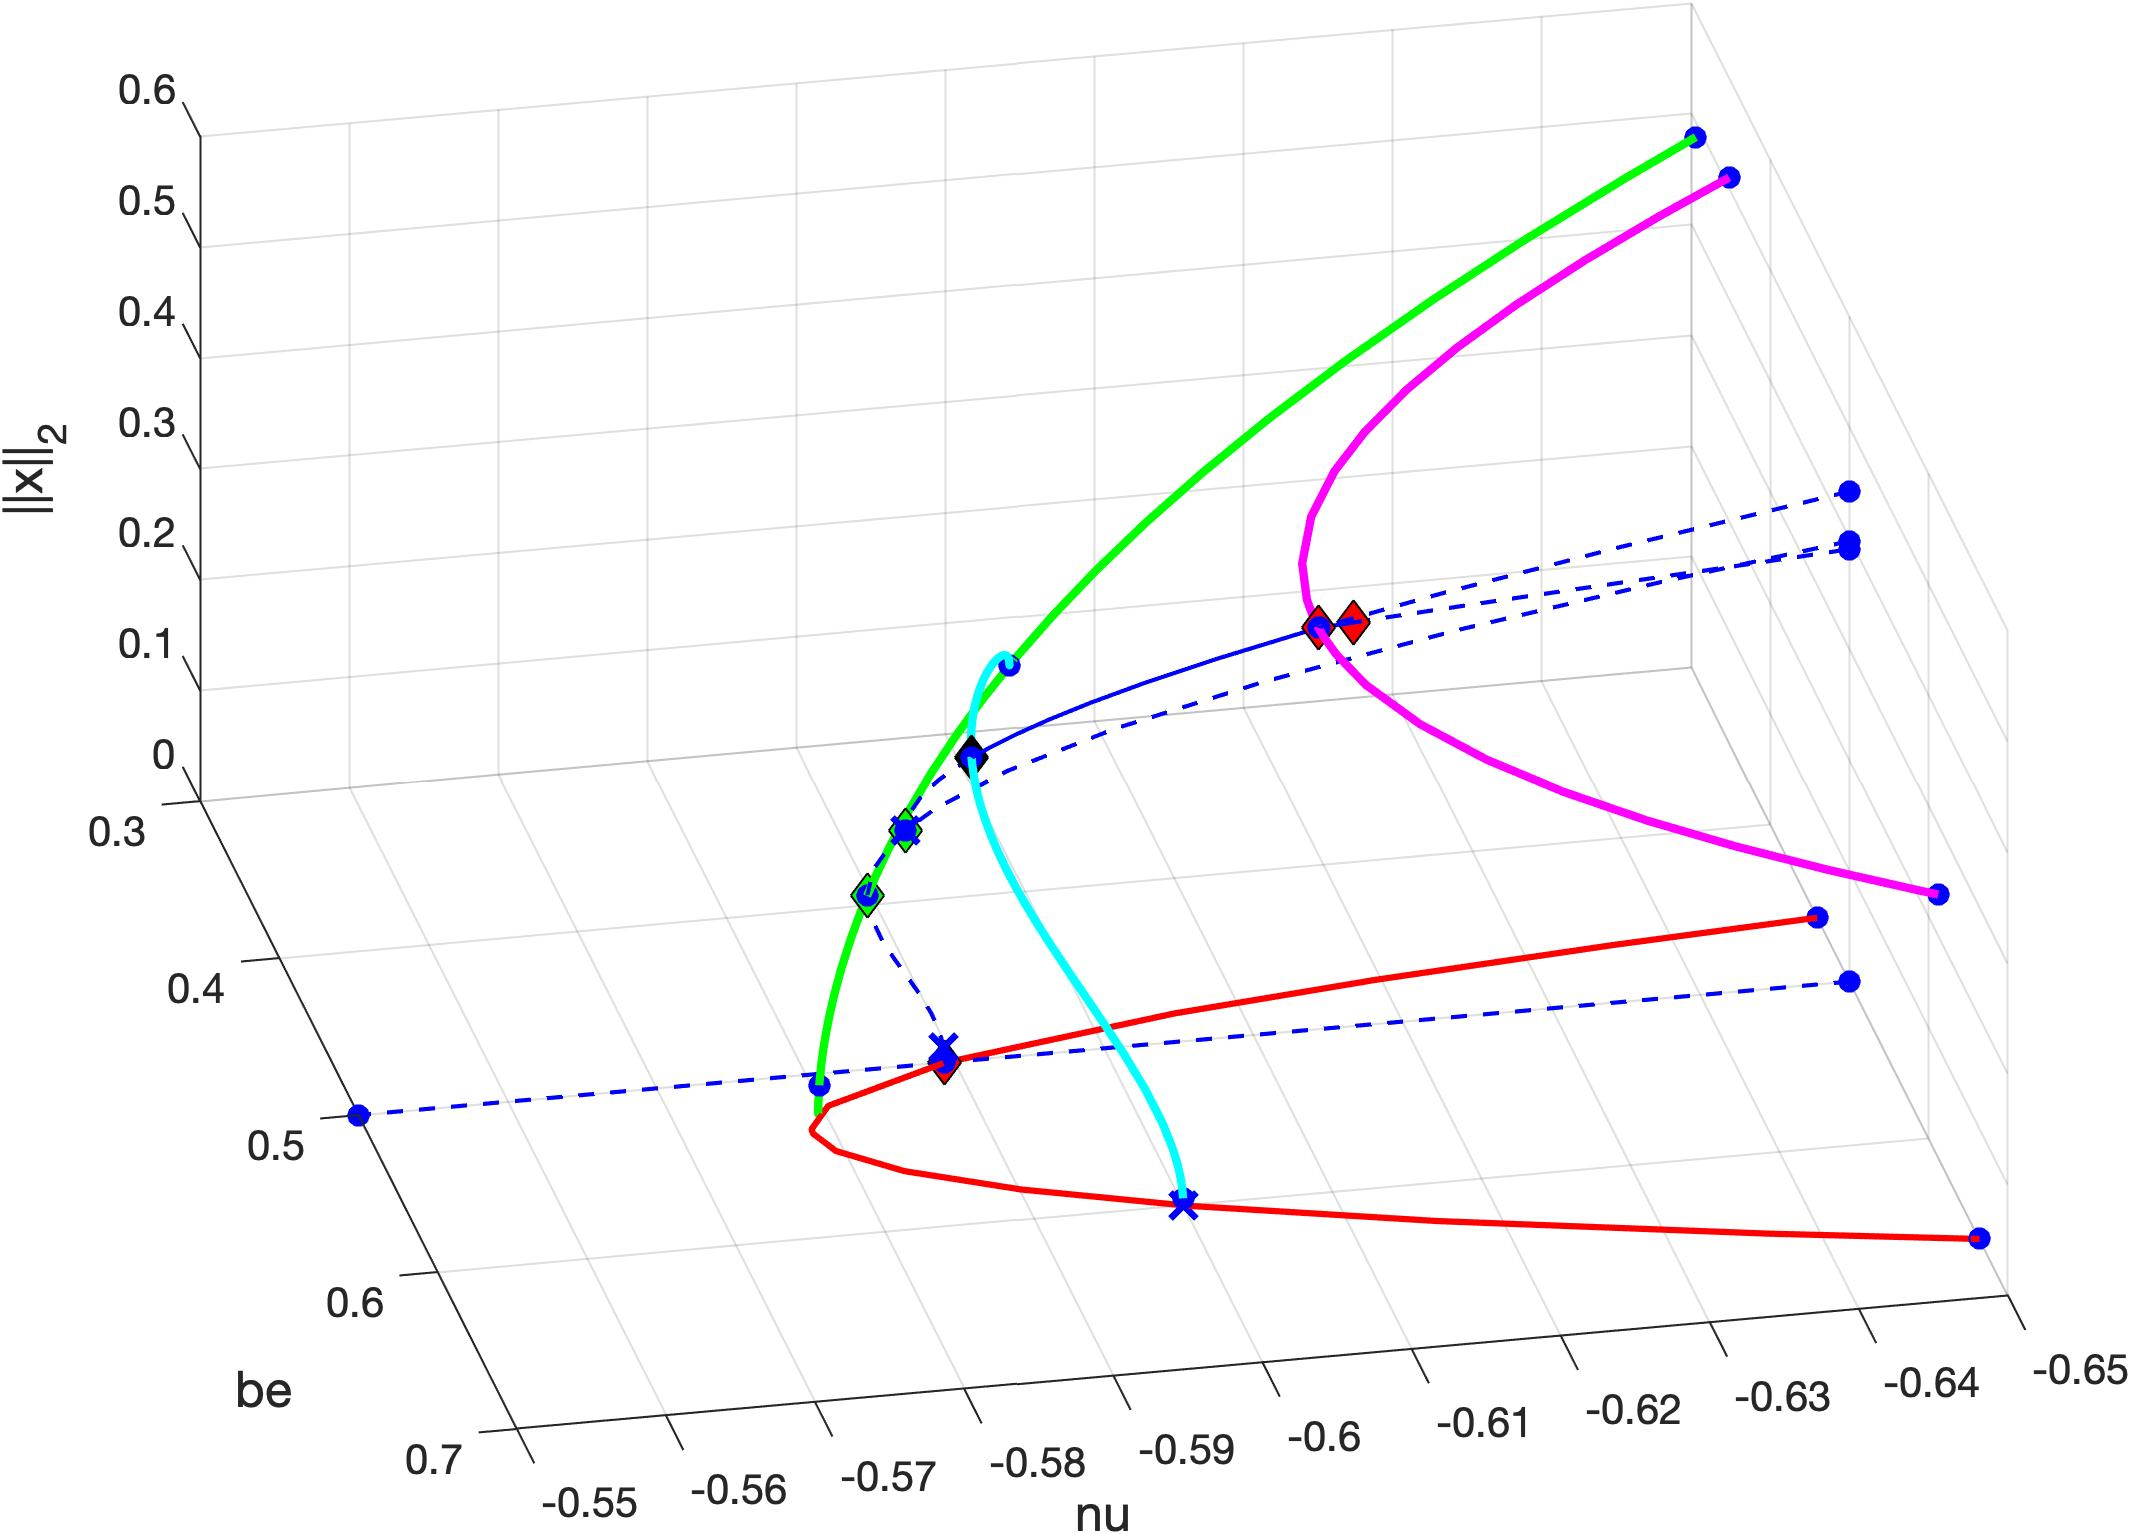
\includegraphics[width=4in]{Figures/Section4_3_1.jpg}
\caption{Bifurcation diagram showing branches of unstable (blue dashed) equilibria, Hopf bifurcations of equilibria (red solid) asymptotically stable (blue solid) and unstable (blue dashed) periodic orbits, saddle-node bifurcations of periodic orbits (green solid), period-doubling bifurcations (magenta solid), and torus bifurcations (cyan solid)  for the vector field in Section~\ref{sec: A web of bifurcations}. The green, blue, and red diamonds along curves of periodic orbits mark saddle-node, torus, and period-doubling bifurcations.}
\label{fig: Section4_3_1}
\end{figure}
Inspection of this diagram shows that the curve of saddle-node bifurcations of periodic orbits terminates on the Hopf bifurcation curve for the equilibrium at the origin, while the curve of torus bifurcations terminates at one end on the curve of saddle-node bifurcations and at the other end on the Hopf bifurcation curve for the equilibrium at the origin.

\section{Post-processing and analysis}
Each successful call to the \mcode{coco} function generates data that is stored to disk (in a subfolder of the \mcode{data} folder identified by the name of the run) and that can be explored using \mcode{coco_plot_bd} or other post-processing utilities. Detailed information about each labeled point is stored in individual solution files, while a less detailed description of all computed points is stored in a separate file as a \textsc{Matlab} cell array. This section shows the use of \textsc{coco} functions for extracting and visualizing stored data.

\subsection{Bifurcation data}
For workspace access to the output cell array, you can assign the output of the \mcode{coco} command to a variable, as shown below.
\begin{lstlisting}[language=coco-highlight,frame=lines]
>> f = @(x,p) p-x.^2;
>> bd = coco('run1', 'ode', 'isol', 'ep', f, 0.5, 'p', 1, 'p', [-1 1]);

    STEP   DAMPING               NORMS              COMPUTATION TIMES
  IT SIT     GAMMA     ||d||     ||f||     ||U||   F(x)  DF(x)  SOLVE
   0                          7.50e-01  1.50e+00    0.0    0.0    0.0
   1   1  3.56e-01  7.50e-01  4.11e-01  1.61e+00    0.0    0.0    0.0
   2   1  1.00e+00  2.68e-01  7.18e-02  1.75e+00    0.0    0.0    0.0
   3   1  1.00e+00  3.47e-02  1.20e-03  1.73e+00    0.0    0.0    0.0
   4   1  1.00e+00  6.02e-04  3.62e-07  1.73e+00    0.0    0.0    0.0
   5   1  1.00e+00  1.81e-07  3.38e-14  1.73e+00    0.0    0.0    0.0

 STEP      TIME        ||U||  LABEL  TYPE             p
    0  00:00:00   1.7321e+00      1  EP      1.0000e+00
   10  00:00:00   9.9654e-02      2          9.7411e-03
   14  00:00:00   1.3380e-06      3  FP      7.8762e-09
   14  00:00:00   1.6856e-08      4  SN      7.8780e-09
   20  00:00:00   2.1653e-01      5          4.3161e-02
   30  00:00:00   1.3657e+00      6          7.4753e-01
   31  00:00:00   1.7321e+00      7  EP      1.0000e+00
\end{lstlisting}
Alternative, load this cell array from disk using the \mcode{coco_bd_read} utility:
\begin{lstlisting}[language=coco-highlight,frame=lines]
>> bd = coco_bd_read('run1');
\end{lstlisting}
You can explore the content of the \mcode{bd} variable in the \textsc{Matlab} variable editor or on the command line. In this example, \mcode{bd} contains $35$ rows and $18$ columns. The top row contains column headers, while the remaining rows contain data.

The command
\begin{lstlisting}[language=coco-highlight,frame=lines]
>> coco_bd_labs('run1', 'SN')

ans =

     4
\end{lstlisting}
returns the labels of all points of type \mcode{SN} in the run \mcode{'run1'}. The same result is returned by replacing \mcode{'run1'} with the corresponding \mcode{bd} output cell array:
\begin{lstlisting}[language=coco-highlight,frame=lines]
>> coco_bd_labs(bd, 'SN')

ans =

     4
\end{lstlisting}
To extract all labels, omit the point type or use \mcode{'all'}:
\begin{lstlisting}[language=coco-highlight,frame=lines]
>> coco_bd_labs('run1', 'all')

ans =

     7     6     5     4     3     2     1
\end{lstlisting}
This is particularly useful if you want to loop over all labels.

Either of the commands
\begin{lstlisting}[language=coco-highlight,frame=lines]
>> coco_bd_lab2idx('run1', 5:7)

ans =

    12     2     1
\end{lstlisting}
and
\begin{lstlisting}[language=coco-highlight,frame=lines]
>> coco_bd_lab2idx(bd, 5:7)

ans =

    12     2     1
\end{lstlisting}
returns the row indices in the data portion of the output cell array from the run \mcode{'run1'} of the points labeled $5$ through $7$. Either of the commands
\begin{lstlisting}[language=coco-highlight,frame=lines]
>> coco_bd_idxs('run1', 'SN')

ans =

    19
\end{lstlisting}
and
\begin{lstlisting}[language=coco-highlight,frame=lines]
>> coco_bd_idxs(bd, 'SN')

ans =

    19
\end{lstlisting}
returns the row indices in the data portion of the output cell array from the run \mcode{'run1'} corresponding to points of type \mcode{SN}. To extract the row indices of all labeled points, omit the point type or use \mcode{'all'}:
\begin{lstlisting}[language=coco-highlight,frame=lines]
>> coco_bd_idxs('run1', 'all')

ans =

     1     2    12    19    20    24    34
\end{lstlisting}

The command
\begin{lstlisting}[language=coco-highlight,frame=lines]
>> p = coco_bd_col('run1', 'p');
\end{lstlisting}
assigns to \mcode{p} all the data in the output cell array associated with the \mcode{'p'} column header. The command
\begin{lstlisting}[language=coco-highlight,frame=lines]
>> px = coco_bd_col('run1', {'p', 'x'});
\end{lstlisting}
assigns to \mcode{px} all the data in the output cell array associated with the \mcode{'p'} and \mcode{'x'} column headers. In general, the output format will depend on the type of data stored in a particular column. To extract data from the output cell array associated with particular column headers, but restricted to labeled points or points of a particular type, use the \mcode{coco_bd_vals} utility as shown below.
\begin{lstlisting}[language=coco-highlight,frame=lines]
>> coco_bd_vals('run1', 'SN', {'p', 'x'})

ans =

   1.0e-07 *

    0.0788
   -0.1265
\end{lstlisting}
To extract data associated with all labeled points, leave the second argument empty, as in
\begin{lstlisting}[language=coco-highlight,frame=lines]
>> coco_bd_vals(bd, [], {'p' 'x'})

ans =

    1.0000    0.7475    0.0432    0.0000    0.0000    0.0097    1.0000
   -1.0000   -0.8646   -0.2078   -0.0000    0.0000    0.0987    1.0000
\end{lstlisting}

The \mcode{coco_print_bd} utility extracts a subset of the content of the output cell array associated with labeled points and particular columns, and prints this to screen or to a file. For example, the command
\begin{lstlisting}[language=coco-highlight,frame=lines]
>> coco_print_bd('run1',  {'p', 'eigs'})

 STEP        ||U||  LABEL  TYPE             p         eigs
   31   1.7321e+00      7  EP      1.0000e+00   2.0000e+00
   30   1.3657e+00      6          7.4753e-01   1.7292e+00
   20   2.1653e-01      5          4.3161e-02   4.1550e-01
   14   1.6856e-08      4  SN      7.8780e-09   2.5298e-08
   14   1.3380e-06      3  FP      7.8762e-09  -2.6760e-06
   10   9.9654e-02      2          9.7411e-03  -1.9739e-01
    0   1.7321e+00      1  EP      1.0000e+00  -2.0000e+00
\end{lstlisting}
includes the values of $p$ and the eigenvalues of the Jacobian of the vector field with respect to the state in the data printed to screen.

The \mcode{coco_plot_bd} utility offers opportunities for additional post-processing prior to visualization. Suppose, for example, that you have executed the command
\begin{lstlisting}[language=coco-highlight,frame=lines]
>> coco('run1', 'ode', 'isol', 'ep', ...
     @brus, [1; 0], {'A' 'B'}, [1; 0], 'B', [0 3]);

    STEP   DAMPING               NORMS              COMPUTATION TIMES
  IT SIT     GAMMA     ||d||     ||f||     ||U||   F(x)  DF(x)  SOLVE
   0                          0.00e+00  1.41e+00    0.0    0.0    0.0

 STEP      TIME        ||U||  LABEL  TYPE             B
    0  00:00:00   1.4142e+00      1  EP      0.0000e+00
    9  00:00:00   3.7417e+00      2  HB      2.0000e+00
   10  00:00:00   4.3853e+00      3          2.3966e+00
   13  00:00:00   5.3852e+00      4  EP      3.0000e+00
\end{lstlisting} 
where the encoding of vector field was given in Section~\ref{sec: Continuing Hopf bifurcations}. Then, the commands
\begin{lstlisting}[language=coco-highlight,frame=lines]
>> clf
>> hold on
>> theme = struct('special', {{'HB'}});
>> coco_plot_bd(theme,'run1', 'B', @(x) [x; x], 'eigs', @(x) real(x))
>> coco_plot_bd(theme,'run1', 'B', @(x) [x; x], 'eigs', @(x) imag(x))
>> grid on
>> hold off
\end{lstlisting}
graph the real and imaginary parts of the eigenvalues of the Jacobian of the vector field with respect to the state versus the parameter $B$ along the curve of equilibria (cf.\ Fig.~\ref{fig: Section5_1_1}).
\begin{figure}[h]
\centering
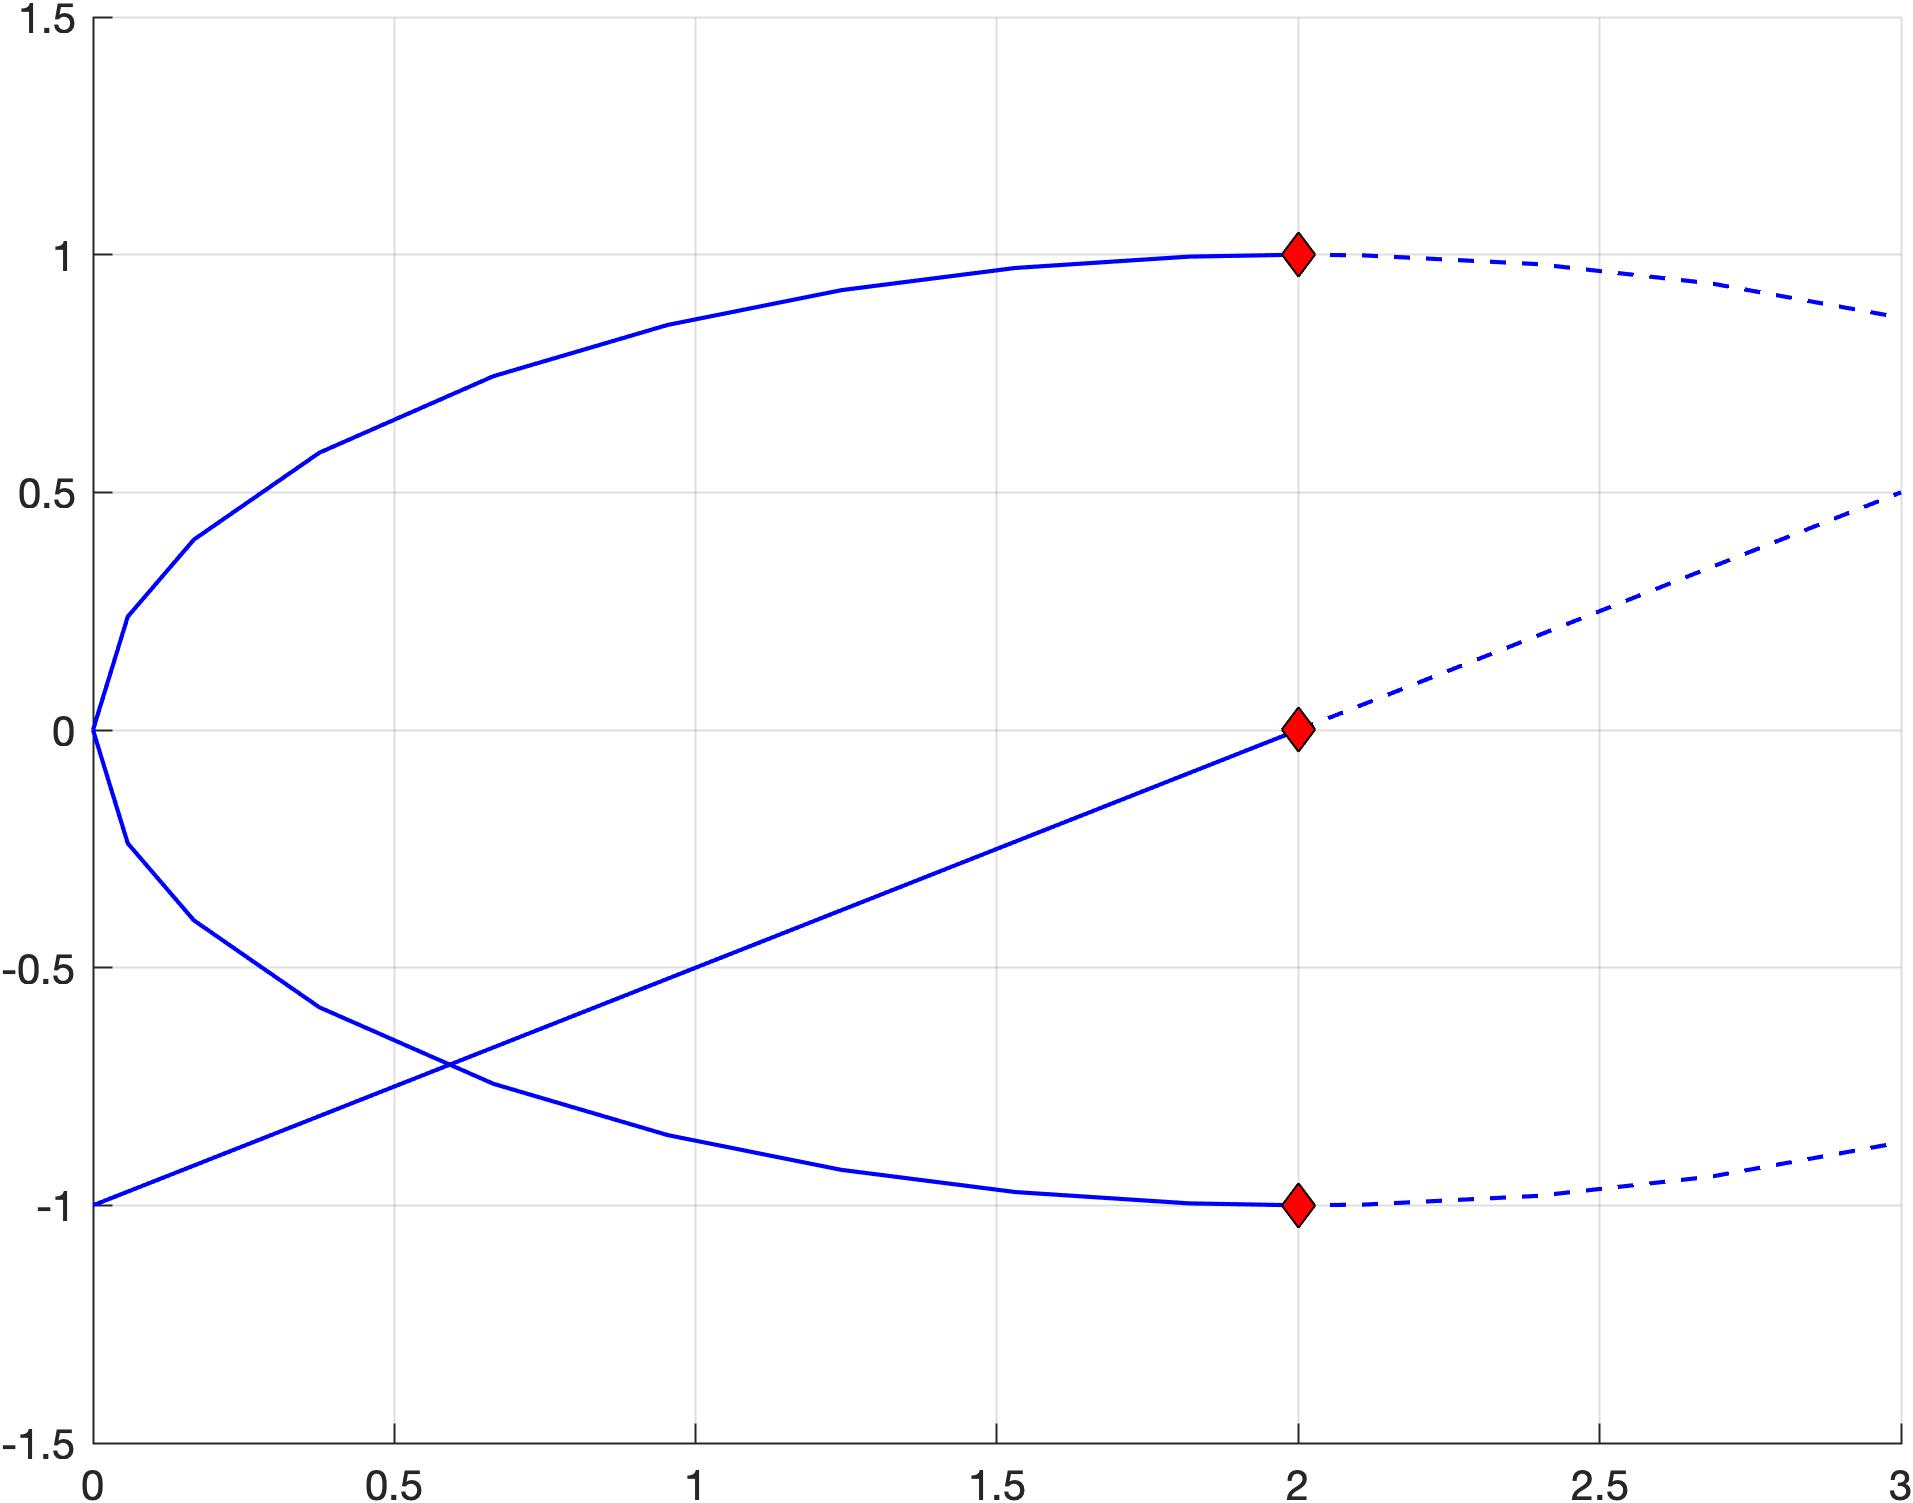
\includegraphics[width=4in]{Figures/Section5_1_1.jpg}
\caption{Bifurcation diagram showing real and imaginary parts of the eigenvalues of the Jacobian of the vector field with respect to the state versus the parameter $B$ for the vector field in Section~\ref{sec: Continuing Hopf bifurcations}. The red diamonds mark the Hopf bifurcation.}
\label{fig: Section5_1_1}
\end{figure}
Alternatively, the commands
\begin{lstlisting}[language=coco-highlight,frame=lines]
>> clf
>> coco_plot_bd(theme,'run1', 'eigs', @(x) real(x), 'eigs', @(x) imag(x))
>> grid on
\end{lstlisting}
show the progression of the eigenvalues in the complex plane during continuation (cf.\ Fig.~\ref{fig: Section5_1_2}).
\begin{figure}[h]
\centering
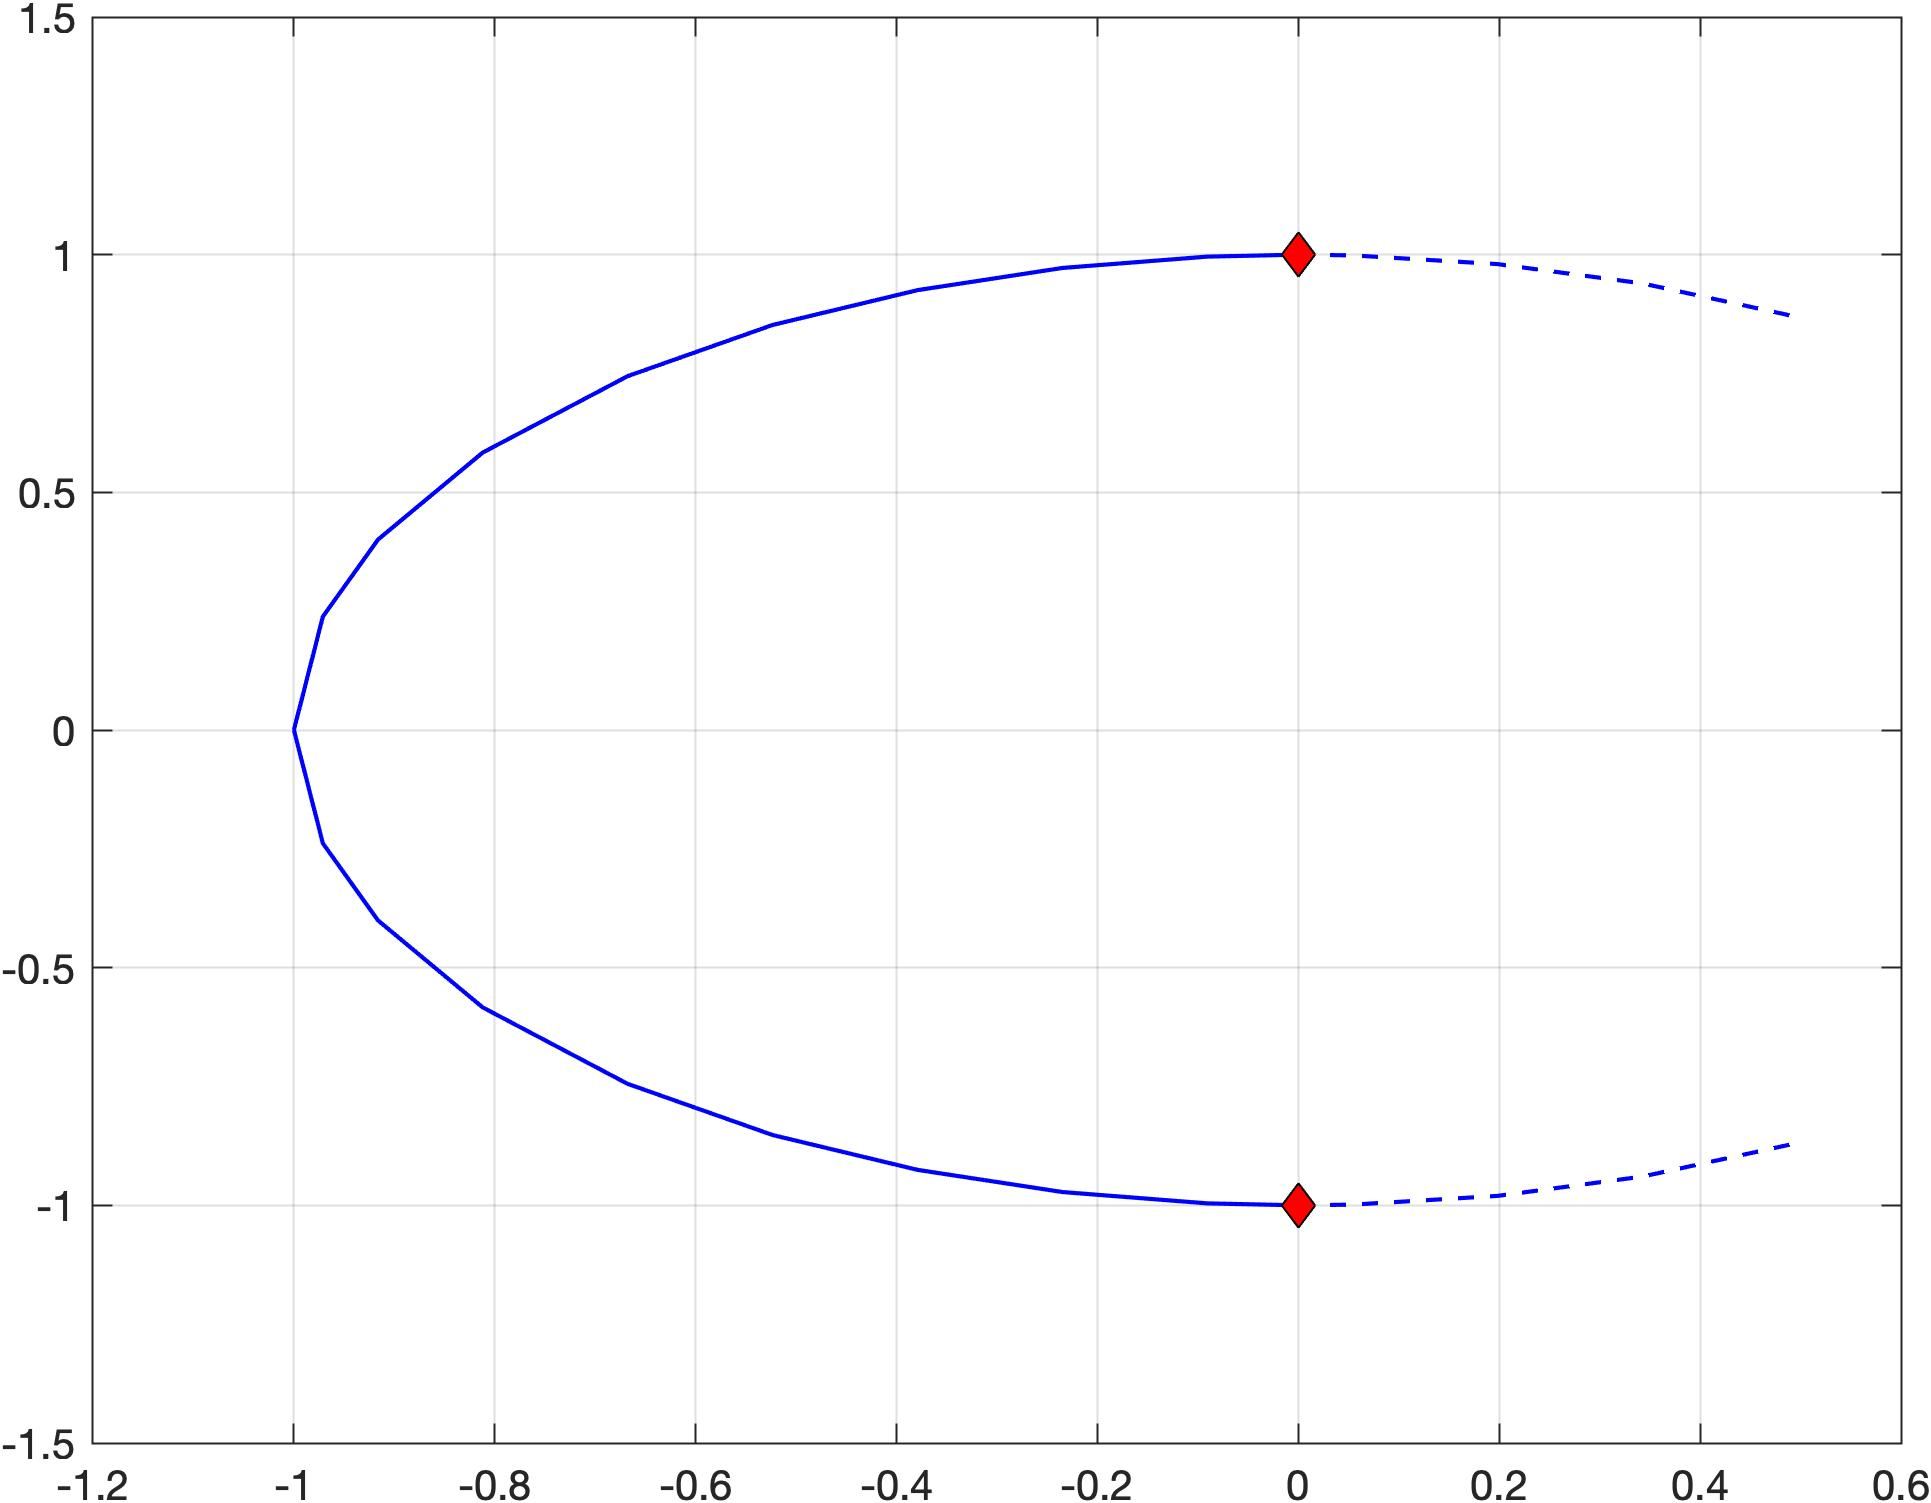
\includegraphics[width=4in]{Figures/Section5_1_2.jpg}
\caption{Bifurcation diagram showing the progression in the complex plane of the eigenvalues of the Jacobian of the vector field with respect to the state versus the parameter $B$ for the vector field in Section~\ref{sec: Continuing Hopf bifurcations}. The red diamonds mark the Hopf bifurcation as the pair of eigenvalues crosses the imaginary axis.}
\label{fig: Section5_1_2}
\end{figure}

\subsection{Individual solutions}
The commands
\begin{lstlisting}[language=coco-highlight,frame=lines]
>> HB = coco_bd_labs('run1', 'HB');
>> sol = ep_read_solution('run1', HB)

sol = 
  struct with fields:

         format: 'ep.v3'
    branch_type: 'ep'
        pt_type: 'HB'
              u: [4x1 double]
              t: [4x1 double]
        ep_test: [1x1 struct]
              x: [2x1 double]
              p: [2x1 double]
             u0: [4x1 double]
             t0: []
            var: [1x1 struct]
             hb: [1x1 struct]
\end{lstlisting}
assigns detailed information about the Hopf bifurcation found in the \mcode{'run1'} run above to the variable \mcode{sol}. As seen below, \mcode{sol.p} and \mcode{sol.x} contain the values of $p$ and $x$ at this point. 
\begin{lstlisting}[language=coco-highlight,frame=lines]
>> sol.x

ans =
    1.0000
    2.0000
    
>> sol.p

ans =
    1.0000
    2.0000
\end{lstlisting}
More interestingly, \mcode{sol.hb.k} contains the squared angular frequency $\omega^2$ associated with the Hopf bifurcation, while the first column of \mcode{sol.var.v} is a unit vector $v$ such that $J^2v+\omega^2v=0$, where $J$ is the Jacobian of the vector field with respect to the state evaluated at the Hopf bifurcation.

A similar syntax applies to the command \mcode{po_read_solution} for accessing data stored to disk during continuation along families of periodic orbits. For example, the commands
\begin{lstlisting}[language=coco-highlight,frame=lines]
>> FP = coco_bd_labs('po_run_SN', 'FP');
>> sol = po_read_solution('po_run_SN', FP)
sol = 
  struct with fields:

         format: 'po.v2'
    branch_type: 'po.SN'
        pt_type: 'FP'
              u: [375x1 double]
              t: [375x1 double]
            tbp: [101x1 double]
            xbp: [101x3 double]
              T: 6.8465
              p: [5x1 double]
            var: [1x1 struct]
             sn: [1x1 struct]
\end{lstlisting}
assigns detailed information about the periodic orbit at the fold point found in Section~\ref{sec: Finding isolated curves} to the variable \mcode{sol}. In this case,  \mcode{sol.p}, \mcode{sol.T}, \mcode{sol.xbp}, and \mcode{sol.tbp} contain the value of $p$, the orbital period, a discretized representation of $x(t)$, and the corresponding temporal mesh, respectively. Individual or families of labeled periodic orbits may be visualized using the \mcode{coco_plot_sol} utility, as shown below (cf.\ Fig.~\ref{fig: Section5_2_1}).
\begin{lstlisting}[language=coco-highlight,frame=lines]
>> clf
>> theme = struct('special', {{'FP'}});
>> coco_plot_sol(theme, 'po_run_SN', '', 'x', 'x', 'x')
>> grid on
\end{lstlisting}
\begin{figure}[h]
\centering
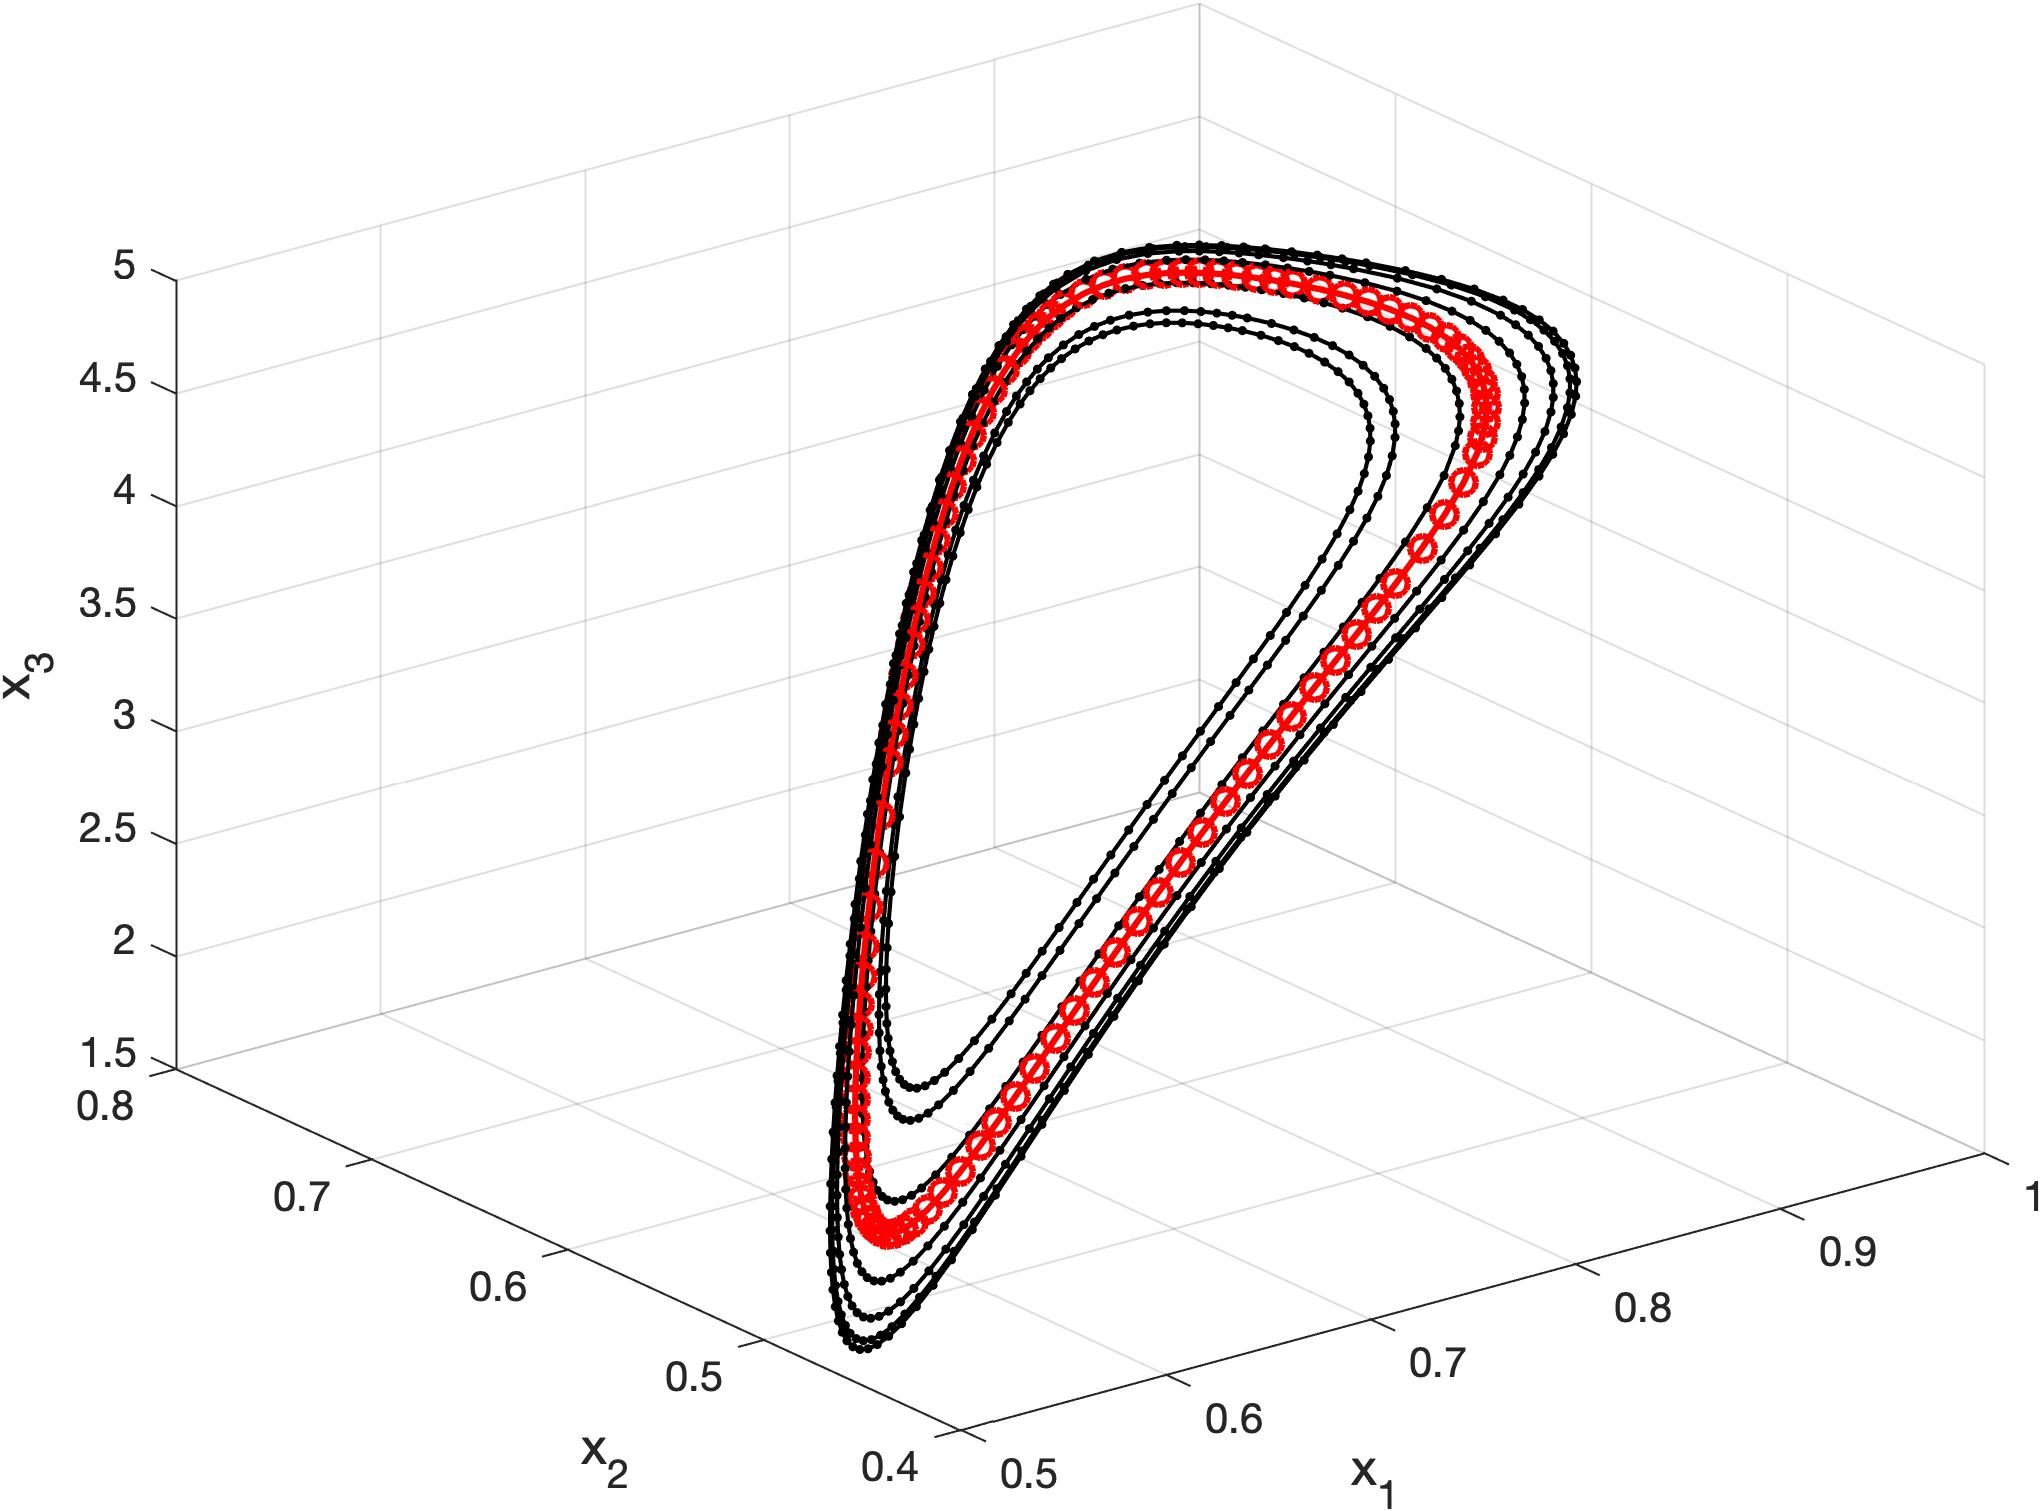
\includegraphics[width=4in]{Figures/Section5_2_1.jpg}
\caption{One-dimensional family of periodic orbits at saddle-node bifurcations for the vector field in Section~\ref{sec: Finding isolated curves}. The orbit found at a fold point along this family is highlighted in solid red.}
\label{fig: Section5_2_1}
\end{figure}

\section{Function definitions}
\subsection{Vector fields}
Consider the following call to \mcode{coco} in terms of a run label \mcode{'run1'}, toolbox family \mcode{'ode'}, initial point type \mcode{'isol'}, branch type \mcode{'ep'}, vector field \mcode{f}, initial numerical value for $x$, parameter name \mcode{'p'}, initial numerical value for $p$, active continuation parameter \mcode{'p'}, and computational domain.
\begin{lstlisting}[language=coco-highlight,frame=lines]
>> coco('run1', 'ode', 'isol', 'ep', f, 0.5, 'p', 1, 'p', [-1 1]);
\end{lstlisting}
By default, \mcode{f} is here assumed to be a handle to a vectorized encoding of a function of two scalar arguments. For example, if the corresponding vector field is given by $f(x,p)=p-x^2$, then \mcode{f} may be given as an anonymous function:
\begin{lstlisting}[language=coco-highlight,frame=lines]
>> f = @(x,p) p-x.^2;
\end{lstlisting}
or as the function handle \mcode{@fold} where \mcode{fold} is encoded in a function file:
\begin{lstlisting}[language=coco-highlight,frame=shadowbox]
function f = fold(x,p)
f = p-x.^2;
end
\end{lstlisting}
The former is convenient for functions that may be easily expressed in terms of a single computational expression, while the latter is necessary when this is not the case. For a vector field that is defined symbolically, a \textsc{coco} interface to the symbolic toolbox in \textsc{Matlab} may be used to generate a corresponding vectorized encoding:
\begin{lstlisting}[language=coco-highlight,frame=lines]
>> syms x p
>> F = sco_sym2funcs(p-x^2, {x, p}, {'x', 'p'});
>> f = F('');
\end{lstlisting}
Finally, rather than a single function handle, the corresponding argument to \mcode{coco} can equal a \textsc{Matlab} struct with a single field \mcode{'f'} whose value equals the function handle, as in
\begin{lstlisting}[language=coco-highlight,frame=lines]
>> f = struct('f', F(''));
>> coco('run1', 'ode', 'isol', 'ep', f, 0.5, 'p', 1, 'p', [-1 1]);
\end{lstlisting}
When vector fields are defined manually (rather than generated symbolically), it is possible, but not encouraged, to build non-vectorized encodings, e.g., 
\begin{lstlisting}[language=coco-highlight,frame=lines]
>> f = @(x,p) p-x^2;
\end{lstlisting}
In this case, it is necessary to alert \mcode{coco} to the non-vectorized encoding by setting the \mcode{'vectorized'} setting to false, as shown in the following commands.
\begin{lstlisting}[language=coco-highlight,frame=lines]
>> prob = coco_prob;
>> prob = coco_set(prob, 'ode', 'vectorized', false);
>> coco(prob, 'run1', 'ode', 'isol', 'ep', f, 0.5, 'p', 1, 'p', [-1 1]);
\end{lstlisting}

%A function handle \mcode{f} to a function with arguments \mcode{x} and \mcode{p} may be recast as a function of arguments \mcode{t} and \mcode{x} provided that the \mcode{p} argument is a constant.
%\begin{lstlisting}[language=coco-highlight,frame=lines]
%>> g = @(t,x) f(x,p0);
%\end{lstlisting}



\subsection{Partial derivatives}
When explicit partial derivatives are available for a vector field, these may be provided to \mcode{coco} and applicable toolbox constructors like \mcode{ode_isol2ep} as shown below.
\begin{lstlisting}[language=coco-highlight,frame=lines]
>> coco('run1', 'ode', 'isol', 'ep', f, dfdx, dfdp, 0.5, 'p', 1, 'p', [-1 1]);
\end{lstlisting}
By default, \mcode{f}, \mcode{dfdx}, and \mcode{dfdp} are assumed to equal handles to vectorized encodings of $f(x,p)$, $\partial_xf(x,p)$, and $\partial_pf(x,p)$. For the case of the fold normal form, these may be defined as anonymous functions
\begin{lstlisting}[language=coco-highlight,frame=lines]
>> f = @(x,p) p-x.^2; dfdx = @(x,p) -2*x; dfdp = @(x,p) ones(1,numel(p));
\end{lstlisting}
or as handles \mcode{@fold}, \mcode{@fold_dx}, and \mcode{@fold_dp}, where \mcode{fold}, \mcode{fold_dx}, and \mcode{fold_dp} are encoded in several function files:
\begin{lstlisting}[language=coco-highlight,frame=shadowbox]
function f = fold(x,p)
f = p-x.^2;
end
\end{lstlisting}
\begin{lstlisting}[language=coco-highlight,frame=shadowbox]
function J = fold_dx(x,p)
J = -2*x;
end
\end{lstlisting}
and
\begin{lstlisting}[language=coco-highlight,frame=shadowbox]
function J = fold_dp(x,p)
J = ones(1,numel(p));
end
\end{lstlisting}
The alternative syntax in terms of a \textsc{Matlab} struct generalizes to this case:
\begin{lstlisting}[language=coco-highlight,frame=lines]
>> f = struct('f', @fold, 'dfdx', @fold_dx, 'dfdp', @fold_dp);
>> coco('run1', 'ode', 'isol', 'ep', f, 0.5, 'p', 1, 'p', [-1 1]);
\end{lstlisting}
Automated generation of such vectorized encodings from a symbolic definition of the vector field is again available using the \textsc{symcoco} interface to the symbolic toolbox in \textsc{Matlab}:
\begin{lstlisting}[language=coco-highlight,frame=lines]
>> syms x p
>> F = sco_sym2funcs(p-x^2, {x, p}, {'x', 'p'});
>> f = struct('f', F(''), 'dfdx', F('x'), 'dfdp', F('p'));
\end{lstlisting}

A similar syntax applies to functions evaluating to higher-order derivatives, although these may get increasingly cumbersome to encode in order to return the required higher-dimensional arrays for vector-valued functions of vector-valued arguments. Given
\[
f(x,p)=\begin{pmatrix}2p_1z^2-2p_5x_1^2-p_3x_1x_2\\p_2z-p_6x_2-p_3x_1x_2\\p_4z-p_4p_7x_3\end{pmatrix},\,z=1-x_1-x_2-x_3
\]
the function files
\begin{lstlisting}[language=coco-highlight,frame=shadowbox]
function f = bykov(x,p)

x1 = x(1,:); 
x2 = x(2,:); 
x3 = x(3,:);
p1 = p(1,:); 
p2 = p(2,:); 
p3 = p(3,:); 
p4 = p(4,:); 
p5 = p(5,:); 
p6 = p(6,:); 
p7 = p(7,:);

z = 1-x1-x2-x3;
f(1,:) = 2*p1.*z.^2-2*p5.*x1.^2-p3.*x1.*x2;
f(2,:) = p2.*z-p6.*x2-p3.*x1.*x2;
f(3,:) = p4.*z-p4.*p7.*x3;

end
\end{lstlisting}
and
\begin{lstlisting}[language=coco-highlight,frame=shadowbox]
function J = bykov_dxdx(x,p)

x1 = x(1,:); 
p1 = p(1,:); 
p3 = p(3,:); 
p5 = p(5,:); 

J = zeros(3,3,3,numel(x1));
J(1,1,1,:) = 4*p1-4*p5;
J(1,1,2,:) = 4*p1-p3;
J(1,1,3,:) = 4*p1;
J(2,1,2,:) = -p3;
J(1,2,1,:) = 4*p1-p3;
J(1,2,2,:) = 4*p1;
J(1,2,3,:) = 4*p1;
J(2,2,1,:) = -p3;
J(1,3,1,:) = 4*p1;
J(1,3,2,:) = 4*p1;
J(1,3,3,:) = 4*p1;

end
\end{lstlisting}
implement vectorized encodings of $f(x,p)$ and the three-dimensional array of second partial derivatives $\partial_{xx}f(x,p)$. The corresponding automated construction is given by the commands
\begin{lstlisting}[language=coco-highlight,frame=lines]
>> syms x1 x2 x3 p1 p2 p3 p4 p5 p6 p7 z
>> z = 1-x1-x2-x3;
>> F = sco_sym2funcs(...
     [2*p1*z^2-2*p5*x1^2-p3*x1*x2; p2*z-p6*x2-p3*x1*x2; p4*z-p7*p4*x3], ...
     {[x1; x2; x3], [p1; p2; p3; p4; p5; p6; p7]}, {'x', 'p'});
>> f = F('');
>> dfdxdx = F({'x','x'});
\end{lstlisting}
as confirmed by the following test:
\begin{lstlisting}[language=coco-highlight,frame=lines]
>> x = rand(3,4); p = rand(7,4);
>> size(f(x,p))
ans =
     3     4
>> size(dfdxdx(x,p))
ans =
     3     3     3     4
>> max(abs(f(x,p)-bykov(x,p)), [], 'all')
ans =
   2.2204e-16
>> max(abs(dfdxdx(x,p)-bykov_dxdx(x,p)), [], 'all')
ans =
   4.4409e-16
\end{lstlisting}

\subsection{Directional derivatives}
\label{sec: Directional derivatives}
The encoding of vector fields and their derivatives generalizes to directional derivatives, e.g.,
\[
(x,p,v)\mapsto D_xf(x,p)[v]:=\left.D_hf(x+hv,p)\right|_{h=0}
\]
and
\[
(x,p,v,w)\mapsto D_{xx}f(x,p)[v,w]:=\left.D_{h_1}D_{h_2}f(x+h_1v+h_2w,p)\right|_{h_1=h_2=0}
\]
in terms of the two- and three-tensors $D_xf(x,p)$ and $D_{xx}f(x,p)$. In the case of the vector field encoded with the symbolic function generator in the previous section, function handles to vectorized encodings of these directional derivatives are assigned to the variables \mcode{Dfdx} and \mcode{Dfdxdx} in the commands shown below.
\begin{lstlisting}[language=coco-highlight,frame=lines]
>> Dfdx = F('x*v');
>> Dfdxdx = F({'x*v','x*v'});
\end{lstlisting}

As an example, we consider the formula\footnote{See Eq.~(5.39) in Kuznetsov, Y.A., \emph{Elements of Applied Bifurcation Theory}, Springer New York, NY, 2004, \url{https://doi.org/10.1007/978-1-4757-3978-7}}
\begin{align*}
(x,p)&\mapsto\frac{1}{2\omega}\Re\bigg(w^{\ast,\mathsf{T}}\cdot\big(D_{xx}f(x,p)\left[v^\ast,\left(2\mathrm{i}\omega I-\partial_xf(x,p)\right)^{-1}\cdot D_{xx}f(x,p)[v,v]\right]\\
&\qquad-2D_{xx}f(x,p)\left[v,(\partial_xf(x,p))^{-1}\cdot D_{xx}f(x,p)\left[v,v^\ast\right]\right]+D_{xxx}f(x,p)\left[v,v,v^\ast\right]\big)\bigg)
\end{align*}
for the \textit{first Lyapunov coefficient} evaluated at a Hopf bifurcation $(x,p)$ in terms of the solutions $\omega$, $v$, and $w$ to the eigenvalue problems
\[
\partial_xf(x,p)\cdot v-\mathrm{i}\omega v=0,\,w^{\ast,\mathsf{T}}\cdot\partial_xf(x,p)-\mathrm{i}\omega w^{\ast,\mathsf{T}}=0
\]
such that $v^{\ast,\mathsf{T}}\cdot v=w^{\ast,\mathsf{T}}\cdot v=1$. The sign of the Lypaunov coefficient determines whether the periodic orbits locally along the branch emanating from the bifurcation are asymptotically stable (negative) or unstable (positive).

It follows from the first eigenvalue problem that, given $x$, $p$, $\omega$, and $\Re(v)$, we obtain
\[
\Im(v)=-\partial_xf(x,p)\cdot \Re(v)/\omega,\,
w^{\ast,\mathsf{T}}=\begin{pmatrix}0 & 1\end{pmatrix}\cdot\begin{pmatrix}\partial_xf(x,p)-\mathrm{i}\omega I & v\\v^{\ast,\mathsf{T}} & 0\end{pmatrix}^{-1}\cdot\begin{pmatrix}I\\0\end{pmatrix}
\]
The function \mcode{lyapunov} below encodes the first Lyapunov coefficient in terms of the arguments \mcode{x} (representing $x$), \mcode{p} (representing $p$), \mcode{v} (representing $\Re(v)$), and \mcode{k} (representing $\omega^2)$.
\begin{lstlisting}[language=coco-highlight,frame=shadowbox]
function y = lyapunov(data, x, p, v, k)

n  = numel(x);
om = sqrt(k);

A  = data.dfdxhan(x,p);
va = v-1i*A*v/om;
va = va/norm(va);
vb = conj(va);
w  = ([A-1i*om*eye(n) va; va' 0]\[eye(n); zeros(1,n)])'*[zeros(n,1); 1];

B = @(dx1, dx2) data.Dfdxdxhan(x, p, dx1, dx2);
C = @(dx1, dx2, dx3) data.Dfdxdxdxhan(x, p, dx1, dx2, dx3);
y = real(w'*(B(vb,(2*1i*om*eye(n)-A)\B(va,va))...
   -2*B(va,A\B(va,vb))+C(va,va,vb)))/2/om;

end
\end{lstlisting}
The \mcode{data} argument is here assumed to be a \textsc{Matlab} struct with fields \mcode{dfdxhan}, \mcode{Dfdxdxhan}, and \mcode{Dfdxdxdxhan} with values given by the function handles \mcode{F('x')}, \mcode{F(\{'x*v','x*v'\})}, and \mcode{F(\{'x*v','x*v','x*v'\})}. 

Consider for example, the following computations.
\begin{lstlisting}[language=coco-highlight,frame=lines]
>> syms x1 x2 A B BB
>> BB = x1*(B-x1*x2);
>> F = sco_sym2funcs([A-BB-x1; BB], {[x1, x2], [A,B]}, {'x', 'p'}, ...
     'maxorder', 3);
>> f = struct('f', F(''), 'dfdx', F('x'), 'dfdp', F('p'));
>> coco('ep_run', 'ode', 'isol', 'ep', ...
     f, [1; 0], {'A' 'B'}, [1; 0], 'B', [0 3]);

    STEP   DAMPING               NORMS              COMPUTATION TIMES
  IT SIT     GAMMA     ||d||     ||f||     ||U||   F(x)  DF(x)  SOLVE
   0                          0.00e+00  1.41e+00    0.0    0.0    0.0

 STEP      TIME        ||U||  LABEL  TYPE             B
    0  00:00:00   1.4142e+00      1  EP      0.0000e+00
    9  00:00:00   3.7417e+00      2  HB      2.0000e+00
   10  00:00:00   4.3853e+00      3          2.3966e+00
   13  00:00:00   5.3852e+00      4  EP      3.0000e+00
   
>> HB  = coco_bd_labs('ep_run', 'HB');
>> sol = ep_read_solution('ep_run', HB);
>> data = struct('dfdxhan', F('x'), 'Dfdxdxhan', F({'x*v','x*v'}), ...
  'Dfdxdxdxhan', F({'x*v','x*v','x*v'}));
>> lyapunov(data, sol.x, sol.p, sol.var.v(:,1), sol.hb.k)

ans =
  -0.5000
\end{lstlisting}
from which we conclude that the Hopf bifurcation is supercritical. We verify this by first continuing along the corresponding branch of periodic orbits:
\begin{lstlisting}[language=coco-highlight,frame=lines]
>> prob = coco_prob;
>> prob = coco_set(prob, 'cont', 'NAdapt', 1);
>> coco(prob, 'po_run', 'ode', 'HB', 'po', 'ep_run', HB, 'B', [0 3])

    STEP   DAMPING               NORMS              COMPUTATION TIMES
  IT SIT     GAMMA     ||d||     ||f||     ||U||   F(x)  DF(x)  SOLVE
   0                          6.21e-06  1.84e+01    0.0    0.0    0.0
   1   1  1.00e+00  2.30e-06  9.65e-14  1.84e+01    0.0    0.0    0.0
   2   1  1.00e+00  3.90e-11  4.71e-15  1.84e+01    0.0    0.0    0.0

 STEP      TIME        ||U||  LABEL  TYPE             B
    0  00:00:00   1.8384e+01      1  EP      2.0000e+00
    1  00:00:00   1.8384e+01      2  FP      2.0000e+00
   10  00:00:00   2.2634e+01      3          2.1169e+00
   20  00:00:01   2.9658e+01      4          2.3641e+00
   30  00:00:02   3.6243e+01      5          2.5973e+00
   40  00:00:03   4.3551e+01      6          2.8198e+00
   50  00:00:03   5.3662e+01      7  EP      3.0000e+00

 STEP      TIME        ||U||  LABEL  TYPE             B
    0  00:00:03   1.8384e+01      8  EP      2.0000e+00
   10  00:00:04   2.2683e+01      9          2.1198e+00
   20  00:00:05   3.2100e+01     10          2.3670e+00
   30  00:00:05   3.6249e+01     11          2.6009e+00
   40  00:00:06   4.5893e+01     12          2.8126e+00
   50  00:00:07   5.3626e+01     13  EP      3.0000e+00
\end{lstlisting}
and then graphing the branches of equilibria and periodic orbits using the following commands (cf.\ Fig.~\ref{fig: Section6_3_1}).
\begin{lstlisting}[language=coco-highlight,frame=lines]
>> figure(1)
>> clf
>> hold on
>> thm = struct();
>> thm.special = {'EP'};
>> coco_plot_bd(thm, 'po_run', 'B', 'MAX(x)', 1)
>> thm.special = {'EP', 'HB'};
>> thm.ylab = 'max(x_1)';
>> coco_plot_bd(thm, 'ep_run', 'B', 'x')
>> grid on
>> hold off
>> axis([0 3 0 inf])
\end{lstlisting}
\begin{figure}[h]
\centering
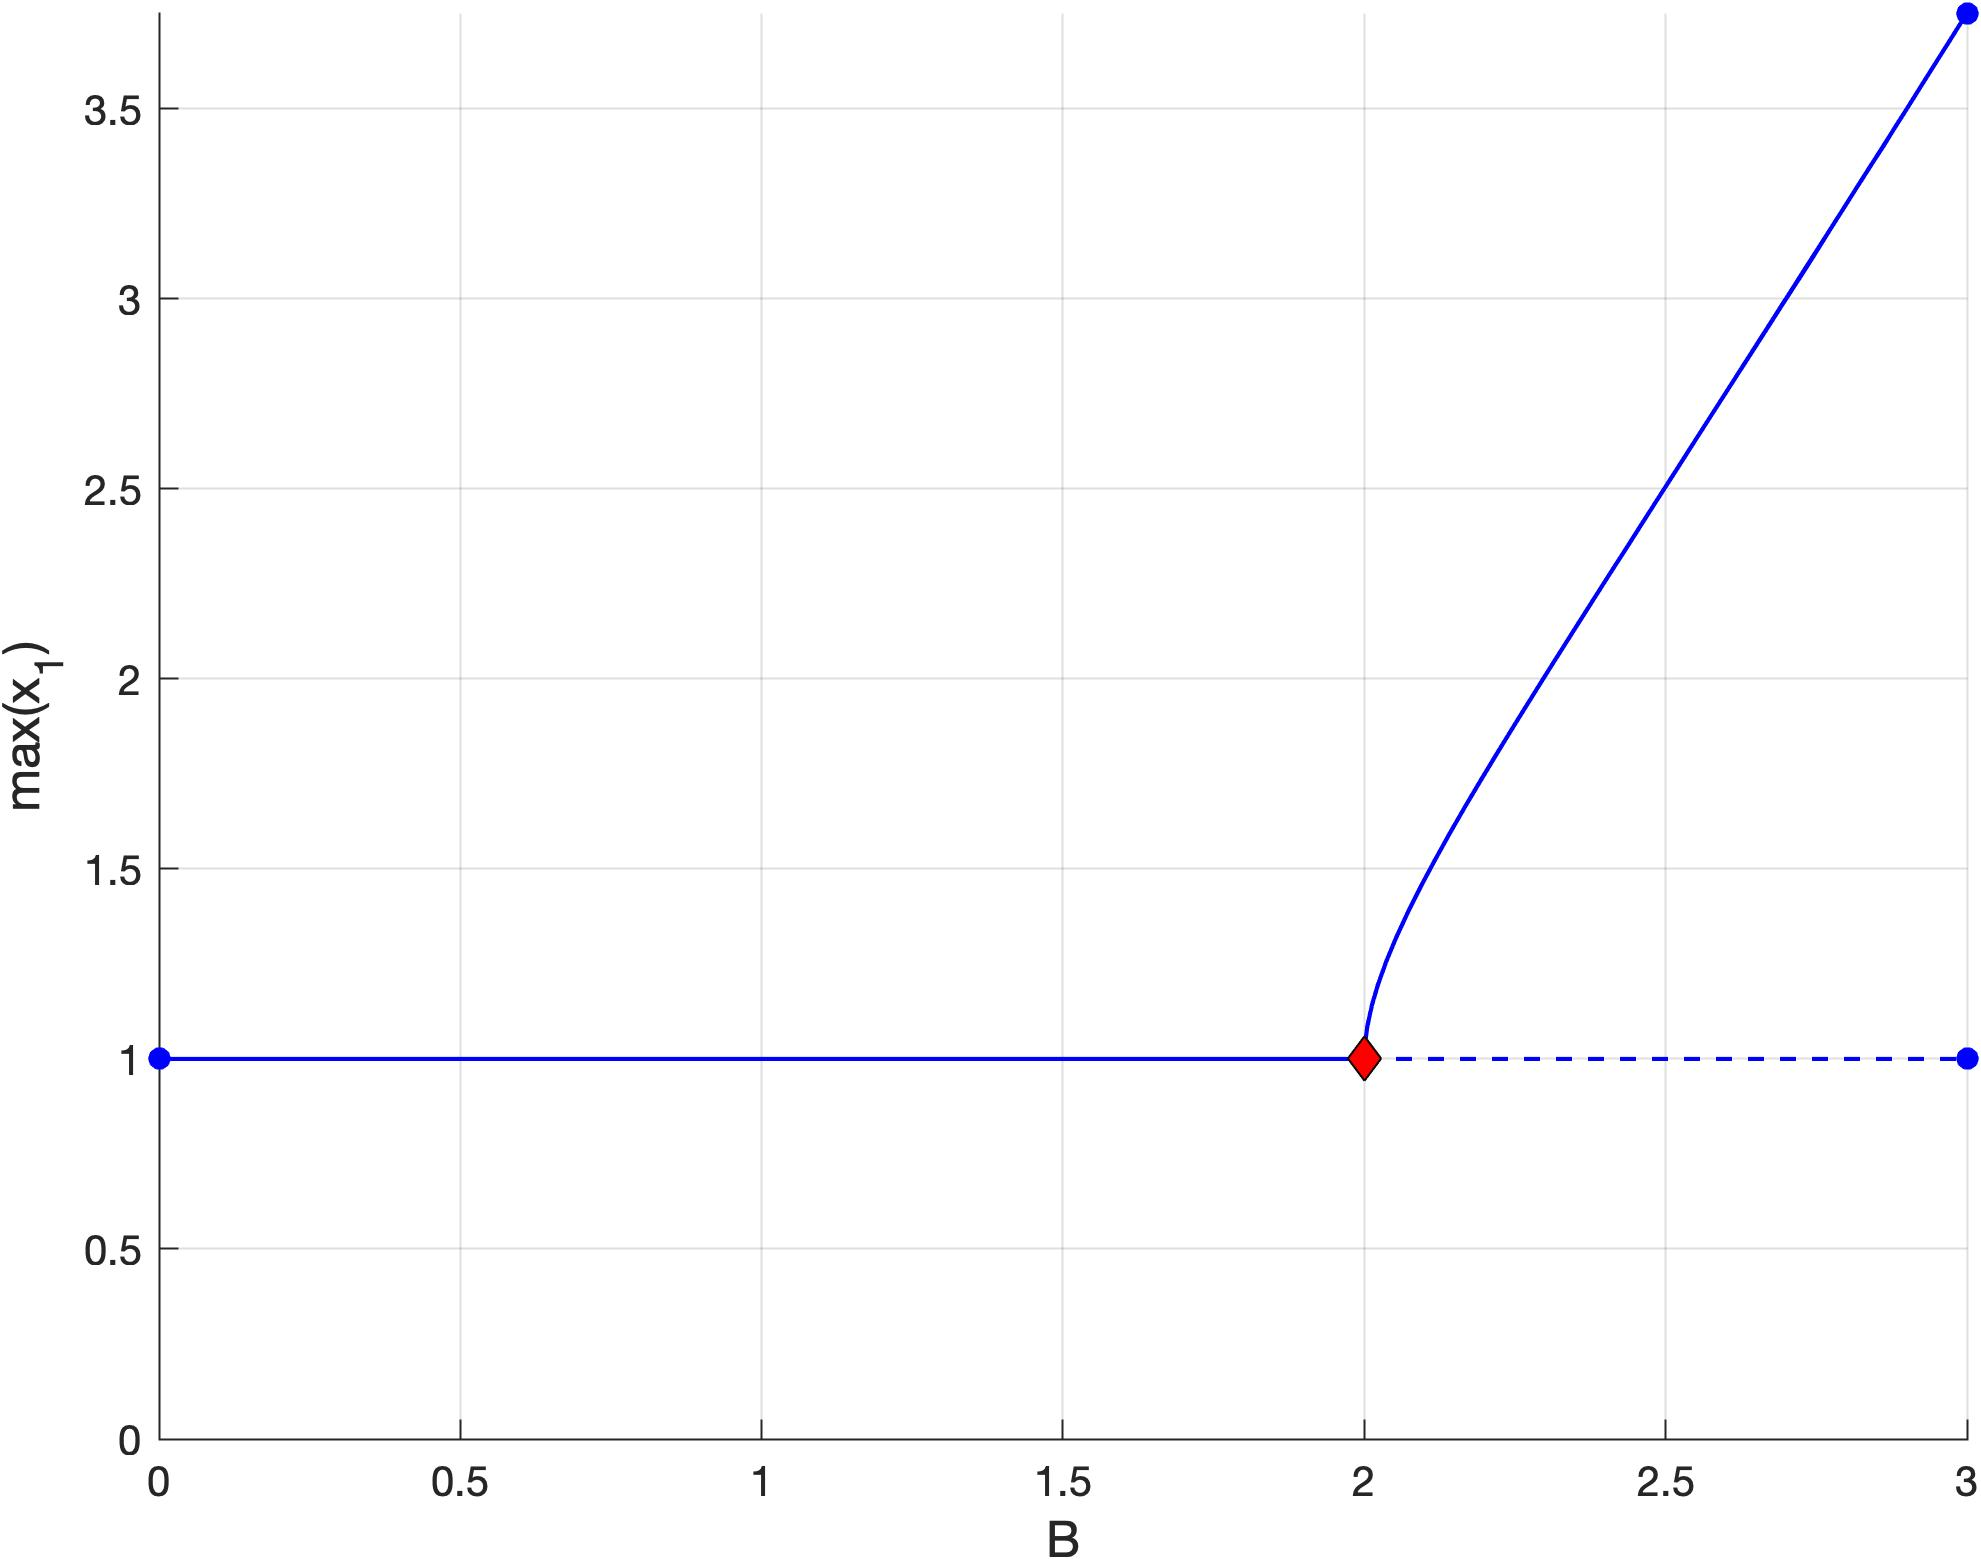
\includegraphics[width=4in]{Figures/Section6_3_1.jpg}
\caption{One-dimensional family of equilibria and one-dimensional family of asymptotically stable periodic orbits emanating from a supercritical Hopf bifurcation (red diamond) for the vector field in Section~\ref{sec: Directional derivatives}.}
\label{fig: Section6_3_1}
\end{figure}
As anticipated, the periodic orbits emanating from the Hopf bifurcation are asymptotically stable.

\section{User-initiated enhancements}
The scope of bifurcation analysis using \textsc{coco} may be expanded through user-initiated enhancements to the default behavior. Such enhancements hint at the full power of the \textsc{coco} package that reaches far beyond a predefined set of problems and analytic functionalities.

\subsection{Monitoring properties of equilibria}
\label{sec: Monitoring properties of equilibria}
You can augment data saved to the output cell array during continuation along a family of equilibria by instructing \textsc{coco} to perform additional computations on each point $(x,p)$ along such a family using the \mcode{ep_add_bddat} constructor.

Suppose, for example, that you have entered the following commands:
\begin{lstlisting}[language=coco-highlight,frame=lines]
>> syms x y s Q1 Q2 Q3 Q4 Q5 Q6 K
>> z  = 1-x-y-s;
>> xp = 2*Q1*z^2-2*Q5*x^2-Q3*x*y;
>> yp = Q2*z-Q6*y-Q3*x*y;
>> sp = Q4*z-K*Q4*s;
>> F = sco_sym2funcs([xp; yp; sp], {[x; y; s], ...
     [Q1; Q2; Q3; Q4; Q5; Q6; K]}, ...
     {'x', 'p'}, 'filename', 'sys_bykov', 'maxorder', 3);
>> x0     = [0.24; 0.04; 0.51];
>> pnames = {'p1' 'p2' 'p3' 'p4' 'p5' 'p6' 'p7'};
>> p0     = [2.5; 0.5; 10; 0.0675; 1; 0.1; 0.4];
>> funcs  = {F(''), F('x'), F('p'), F({'x','x'}), F({'x','p'}), F({'p','p'})};
>> prob = coco_prob;
>> prob = ode_isol2ep(prob, '', funcs{:}, x0, pnames, p0);
>> eprunid = 'ep_run';
\end{lstlisting}
Here, you used the \mcode{ode_isol2ep} constructor to initialize the search for equilibrium points of the vector field
\[
f(x,p)=\begin{pmatrix}2p_1z^2-2p_5x_1^2-p_3x_1x_2\\p_2z-p_6x_2-p_3x_1x_2\\p_4z-p_4p_7x_3\end{pmatrix},\,z=1-x_1-x_2-x_3
\]
The default behavior of \textsc{coco} produces the output shown below.
\begin{lstlisting}[language=coco-highlight,frame=lines]
>> coco(prob, eprunid, [], 'p2', [0.4 3]);

    STEP   DAMPING               NORMS              COMPUTATION TIMES
  IT SIT     GAMMA     ||d||     ||f||     ||U||   F(x)  DF(x)  SOLVE
   0                          1.06e-02  1.04e+01    0.0    0.0    0.0
   1   1  1.00e+00  5.46e-03  1.13e-04  1.04e+01    0.0    0.0    0.0
   2   1  1.00e+00  6.56e-05  5.26e-09  1.04e+01    0.0    0.0    0.0
   3   1  1.00e+00  3.84e-09  3.12e-17  1.04e+01    0.0    0.0    0.0

 STEP      TIME        ||U||  LABEL  TYPE            p2
    0  00:00:00   1.0404e+01      1  EP      5.0000e-01
    2  00:00:00   1.0396e+01      2  EP      4.0000e-01

 STEP      TIME        ||U||  LABEL  TYPE            p2
    0  00:00:00   1.0404e+01      3  EP      5.0000e-01
   10  00:00:00   1.0483e+01      4          1.0395e+00
   11  00:00:00   1.0483e+01      5  HB      1.0410e+00
   17  00:00:01   1.0485e+01      6  FP      1.0522e+00
   17  00:00:01   1.0485e+01      7  SN      1.0522e+00
   20  00:00:01   1.0485e+01      8          1.0447e+00
   21  00:00:01   1.0485e+01      9  SN      1.0420e+00
   21  00:00:01   1.0485e+01     10  FP      1.0421e+00
   23  00:00:01   1.0489e+01     11  HB      1.0516e+00
   30  00:00:02   1.0506e+01     12          1.1183e+00
   40  00:00:02   1.0831e+01     13          2.1406e+00
   43  00:00:02   1.1235e+01     14  EP      3.0000e+00
\end{lstlisting}
The call to \mcode{ep_add_bddat} below modifies the default behavior to include a column in the output cell array and in the screen output with the smallest singular value of the Jacobian $\partial_xf(x,p)$ at each equilibrium point.
\begin{lstlisting}[language=coco-highlight,frame=lines]
>> prob = ep_add_bddat(prob, '', 'svds', ...
     @(d,x,p) min(svds(feval(F('x'),x,p))));
>> coco(prob, eprunid, [], 'p2', [0.4 3]);

    STEP   DAMPING               NORMS              COMPUTATION TIMES
  IT SIT     GAMMA     ||d||     ||f||     ||U||   F(x)  DF(x)  SOLVE
   0                          1.06e-02  1.04e+01    0.0    0.0    0.0
   1   1  1.00e+00  5.46e-03  1.13e-04  1.04e+01    0.0    0.0    0.0
   2   1  1.00e+00  6.56e-05  5.26e-09  1.04e+01    0.0    0.0    0.0
   3   1  1.00e+00  3.84e-09  3.12e-17  1.04e+01    0.0    0.0    0.0

 STEP      TIME        ||U||  LABEL  TYPE            p2        svds
    0  00:00:00   1.0404e+01      1  EP      5.0000e-01  4.4953e-02
    2  00:00:00   1.0396e+01      2  EP      4.0000e-01  4.5111e-02

 STEP      TIME        ||U||  LABEL  TYPE            p2        svds
    0  00:00:00   1.0404e+01      3  EP      5.0000e-01  4.4953e-02
   10  00:00:00   1.0483e+01      4          1.0395e+00  1.1742e-02
   11  00:00:00   1.0483e+01      5  HB      1.0410e+00  1.0802e-02
   17  00:00:01   1.0485e+01      6  FP      1.0522e+00  3.9708e-08
   17  00:00:01   1.0485e+01      7  SN      1.0522e+00  6.0449e-09
   20  00:00:01   1.0485e+01      8          1.0447e+00  2.3490e-03
   21  00:00:01   1.0485e+01      9  SN      1.0420e+00  6.9403e-07
   21  00:00:01   1.0485e+01     10  FP      1.0421e+00  8.7757e-06
   23  00:00:01   1.0489e+01     11  HB      1.0516e+00  1.2221e-02
   30  00:00:02   1.0506e+01     12          1.1183e+00  4.6977e-02
   40  00:00:02   1.0831e+01     13          2.1406e+00  2.2317e-02
   43  00:00:02   1.1235e+01     14  EP      3.0000e+00  2.1167e-02
\end{lstlisting}
As expected, this value is approximately $0$ at a saddle-node bifurcation.

Either of the Hopf bifurcations found in the previous run may be used to restart continuation along a family of Hopf bifurcations, as exemplified below.
\begin{lstlisting}[language=coco-highlight,frame=lines]
>> labs = coco_bd_labs(eprunid, 'HB');
>> prob = coco_prob;
>> prob = ode_HB2HB(prob, '', eprunid, labs(1));
>> prob = coco_set(prob, 'cont', 'PtMX', [90 0]);
>> hbrunid = 'HB-curve';
>> coco(prob, hbrunid, [], {'p2' 'p7'}, {[0.4 3], [0 8]});

    STEP   DAMPING               NORMS              COMPUTATION TIMES
  IT SIT     GAMMA     ||d||     ||f||     ||U||   F(x)  DF(x)  SOLVE
   0                          9.23e-08  1.05e+01    0.0    0.0    0.0

 STEP      TIME        ||U||  LABEL  TYPE            p2           p7
    0  00:00:00   1.0538e+01      1  EP      1.0410e+00   4.0000e-01
   10  00:00:00   1.0480e+01      2          7.1662e-01   1.6805e-01
   11  00:00:00   1.0480e+01      3  FP      7.1639e-01   1.6698e-01
   20  00:00:01   1.0486e+01      4          7.6656e-01   1.7425e-01
   30  00:00:01   1.0550e+01      5          1.0661e+00   4.2629e-01
   36  00:00:02   1.0605e+01      6  BTP     1.1612e+00   7.2234e-01
   40  00:00:02   1.0880e+01      7          1.2603e+00   1.7835e+00
   43  00:00:02   1.1183e+01      8  BP      1.2952e+00   2.5338e+00
   50  00:00:03   1.3021e+01      9          1.4705e+00   5.3034e+00
   60  00:00:03   1.3468e+01     10          1.5984e+00   5.8039e+00
   70  00:00:04   1.3332e+01     11          1.6524e+00   5.6316e+00
   76  00:00:04   1.2079e+01     12  FP      1.7317e+00   3.9579e+00
   80  00:00:04   1.1277e+01     13          1.6891e+00   2.5468e+00
   85  00:00:05   1.0695e+01     14  BP      1.4186e+00   9.7401e-01
   85  00:00:05   1.0694e+01     15  BTP     1.4176e+00   9.7140e-01
   90  00:00:05   1.0534e+01     16  EP      1.0229e+00   3.8396e-01
\end{lstlisting}
By default, \textsc{coco} solves for the square of the limiting angular frequency of oscillation along the family of periodic orbits emanating from such a bifurcation point, but does not store this data in the output cell array. The following sequence of commands modifies this behavior.
\begin{lstlisting}[language=coco-highlight,frame=lines]
>> prob = ep_HB_add_bddat(prob, '', 'freq', @(d,x,p,v,k) sqrt(max(k,0)));
>> coco(prob, hbrunid, [], {'p2' 'p7'}, {[0.4 3], [0 8]});

    STEP   DAMPING               NORMS              COMPUTATION TIMES
  IT SIT     GAMMA     ||d||     ||f||     ||U||   F(x)  DF(x)  SOLVE
   0                          9.23e-08  1.05e+01    0.0    0.0    0.0

 STEP     ...   LABEL  TYPE            p2           p7        freq
    0    ...       1  EP      1.0410e+00   4.0000e-01  5.9106e-02
   10    ...       2          7.1662e-01   1.6805e-01  5.6765e-02
   11    ...       3  FP      7.1639e-01   1.6698e-01  5.6779e-02
   20    ...       4          7.6656e-01   1.7425e-01  5.7636e-02
   30    ...       5          1.0661e+00   4.2629e-01  4.9090e-02
   36    ...       6  BTP     1.1612e+00   7.2234e-01  0.0000e+00
   40    ...       7          1.2603e+00   1.7835e+00  0.0000e+00
   43    ...       8  BP      1.2952e+00   2.5338e+00  0.0000e+00
   50    ...       9          1.4705e+00   5.3034e+00  0.0000e+00
   60    ...      10          1.5984e+00   5.8039e+00  0.0000e+00
   70    ...      11          1.6524e+00   5.6316e+00  0.0000e+00
   76    ...      12  FP      1.7317e+00   3.9579e+00  0.0000e+00
   80    ...      13          1.6891e+00   2.5468e+00  0.0000e+00
   85    ...      14  BP      1.4186e+00   9.7401e-01  0.0000e+00
   85    ...      15  BTP     1.4176e+00   9.7140e-01  2.8516e-05
   90    ...      16  EP      1.0229e+00   3.8396e-01  5.9254e-02
\end{lstlisting}
Here, the frequency is reported as $0$ at neutral saddle points, which satisfy the algebraic conditions for a Hopf bifurcation but not the condition that there exist a pair of imaginary, complex conjugate eigenvalues of $\partial_xf(x,p)$.

As illustrated below, a further modification appends information about the first Lyapunov coefficient to the output cell array and the screen output.
\begin{lstlisting}[language=coco-highlight,frame=lines]
>> data = struct('dfdxhan', F('x'), 'Dfdxdxhan', F({'x*v','x*v'}), ...
     'Dfdxdxdxhan', F({'x*v','x*v','x*v'}), 'nanflag', 1);
>> prob = ep_HB_add_bddat(prob, '', 'L1', @lyapunov, 'data', data);
>> prob = coco_set(prob, 'cont', 'PtMX', [90 0]);
>> coco(prob, hbrunid, [], {'p2' 'p7'}, {[0.4 3], [0 8]});

    STEP   DAMPING               NORMS              COMPUTATION TIMES
  IT SIT     GAMMA     ||d||     ||f||     ||U||   F(x)  DF(x)  SOLVE
   0                          9.23e-08  1.05e+01    0.0    0.0    0.0

 STEP    ...   LABEL  TYPE            p2           p7        freq          L1
    0    ...       1  EP      1.0410e+00   4.0000e-01  5.9106e-02  7.3283e+01
   10    ...       2          7.1662e-01   1.6805e-01  5.6765e-02 -1.2709e+02
   11    ...       3  FP      7.1639e-01   1.6698e-01  5.6779e-02 -1.2680e+02
   20    ...       4          7.6656e-01   1.7425e-01  5.7636e-02 -8.6324e+01
   30    ...       5          1.0661e+00   4.2629e-01  4.9090e-02  2.5779e+02
   36    ...       6  BTP     1.1612e+00   7.2234e-01  0.0000e+00         NaN
   40    ...       7          1.2603e+00   1.7835e+00  0.0000e+00         NaN
   43    ...       8  BP      1.2952e+00   2.5338e+00  0.0000e+00         NaN
   50    ...       9          1.4705e+00   5.3034e+00  0.0000e+00         NaN
   60    ...      10          1.5984e+00   5.8039e+00  0.0000e+00         NaN
   70    ...      11          1.6524e+00   5.6316e+00  0.0000e+00         NaN
   76    ...      12  FP      1.7317e+00   3.9579e+00  0.0000e+00         NaN
   80    ...      13          1.6891e+00   2.5468e+00  0.0000e+00         NaN
   85    ...      14  BP      1.4186e+00   9.7401e-01  0.0000e+00         NaN
   85    ...      15  BTP     1.4176e+00   9.7140e-01  2.8516e-05 -9.3424e+13
   90    ...      16  EP      1.0229e+00   3.8396e-01  5.9254e-02  6.0838e+01
\end{lstlisting}
where \mcode{lyapunov} is a slight modification of the function shown in the previous section that returns \mcode{NaN} in the event of a neutral saddle, as shown below.
\begin{lstlisting}[language=coco-highlight,frame=shadowbox]
function y = lyapunov(data, x, p, v, k)

n  = numel(x);
om = sqrt(k);
if om<1e-6 && data.nanflag % if neutral saddle
  y = NaN;
  return
end

A  = data.dfdxhan(x,p);
va = v-1i*A*v/om;
va = va/norm(va);
vb = conj(va);
w  = ([A-1i*om*eye(n) va; va' 0]\[eye(n); zeros(1,n)])'...
  *[zeros(n,1); 1];

B = @(dx1, dx2) data.Dfdxdxhan(x, p, dx1, dx2);
C = @(dx1, dx2, dx3) data.Dfdxdxdxhan(x, p, dx1, dx2, dx3); 
y = real(w'*(B(vb,(2*1i*om*eye(n)-A)\B(va,va))...
  -2*B(va,A\B(va,vb))+C(va,va,vb)))/2/om;

end
\end{lstlisting}
We visualize the results of this analysis, including a curve of saddle-node bifurcations, using the following commands.
\begin{lstlisting}[language=coco-highlight,frame=lines]
>> figure(1)
>> clf
>> hold on
>> thm = struct();
>> thm.special = {'HB', 'SN'};
>> coco_plot_bd(thm, eprunid, 'p2', 'x')
>> coco_plot_bd(snrunid, 'p2', 'x')
>> thm = struct();
>> thm.special = {'BTP'};
>> thm.ustab = 'L1';
>> thm.ustabfun = @(x) 1+(~isnan(x) & x>0)+2*isnan(x);
>> thm.usept = {};
>> thm.lspec = {{'r-', 'LineWidth', 1.5}, {'r-.', 'LineWidth', 1.5}};
>> thm.xlab  = 'p_2';
>> coco_plot_bd(thm, hbrunid, 'p2', 'x')
>> hold off
>> grid on
>> axis([0.5 2 0 0.16])
\end{lstlisting}
Here, the sign of the Lyapunov coefficient is used to select the line style for the curve of Hopf bifurcations.
\begin{figure}[h]
\centering
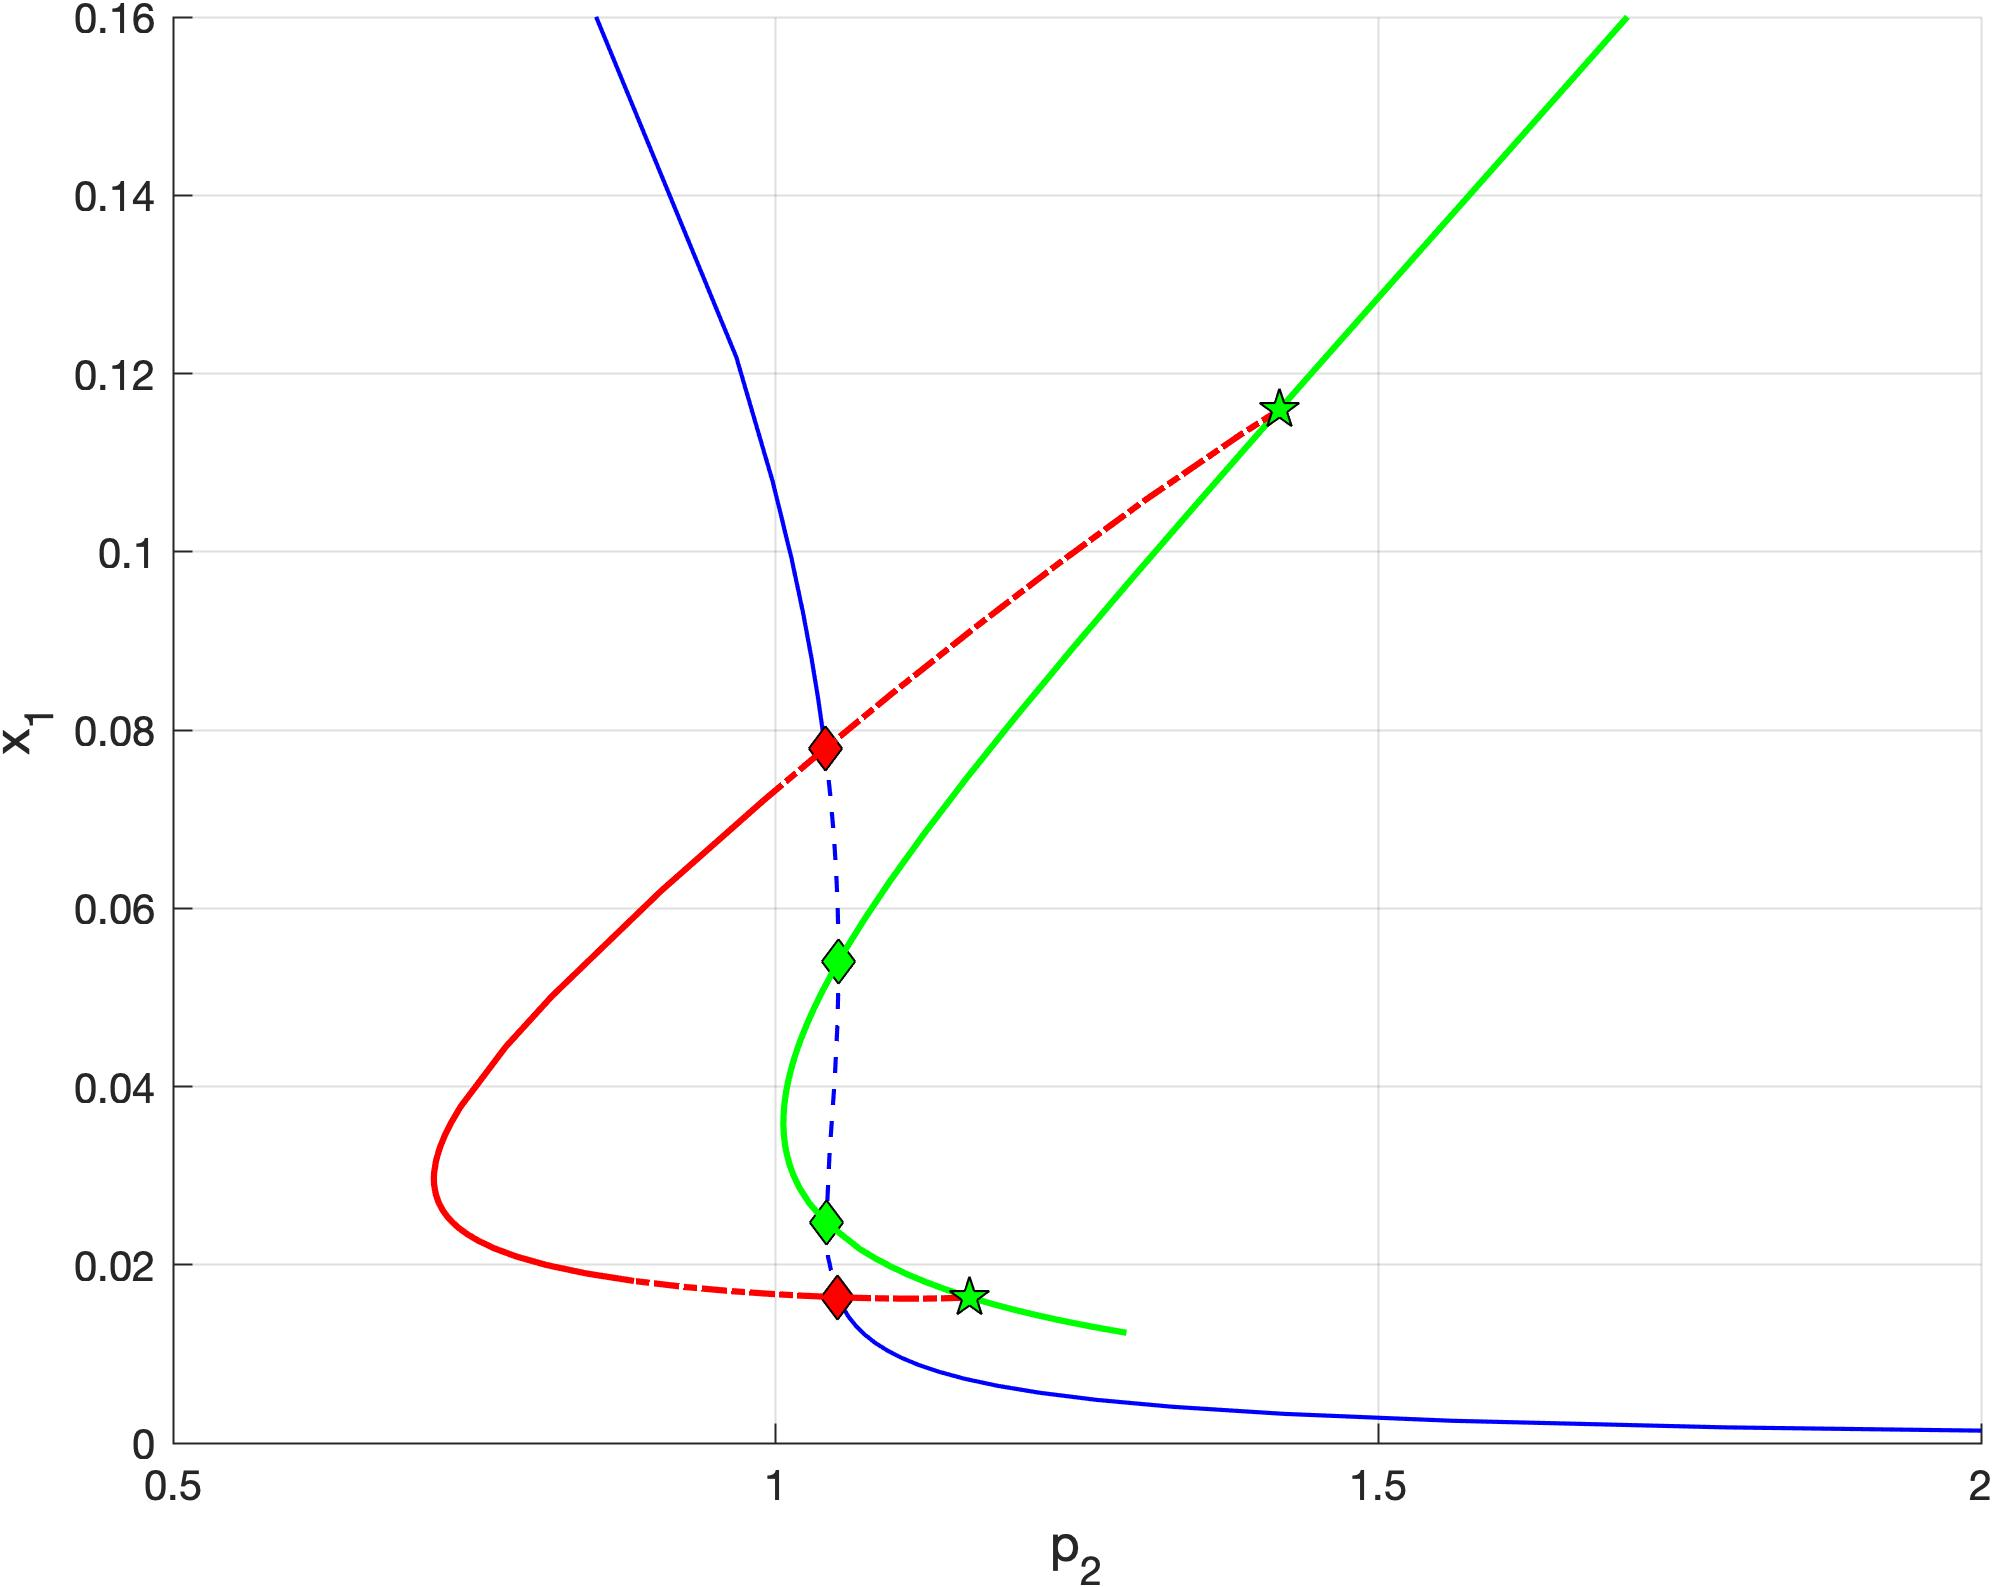
\includegraphics[width=4in]{Figures/Section7_1_1.jpg}
\caption{Families of equilibria (blue), saddle-node bifurcations of equilibria (green), and Hopf bifurcations of equilibria (red) for the vector field in Section~\ref{sec: Monitoring properties of equilibria}. The Hopf bifurcation curve terminates at each end on the saddle-node bifurcation curve at a Bogdanov-Takens points (green star) and consists of both subcritical (dash-dotted) and supercritical (solid) bifurcations.}
\label{fig: Section7_1_1}
\end{figure}

\subsection{Continuing generalized Hopf bifurcations}
\label{sec: Continuing generalized Hopf bifurcations}

Computations added using \mcode{ep_add_bddat}, \mcode{ep_SN_add_bddat}, and \mcode{ep_HB_add_bddat},  execute after convergence to an equilibrium, saddle-node bifurcation, or Hopf bifurcation, respectively. They allow you to perform \textit{a posteriori} evaluation of properties of each solution point but cannot be used to automatically detect special points associated with particular numerical thresholds. To detect such special points during continuation of Hopf bifurcations, embed the monitor functions within the continuation problem using the \mcode{ep_HB_add_func} constructor. 

As an example, zero crossings of the first Lyapunov coefficient along a curve of Hopf bifurcations may be detected by embedding the \mcode{lyapunov} function as a \mcode{'regular'} monitor function, as in the following example code.
\begin{lstlisting}[language=coco-highlight,frame=lines]
>> prob = coco_prob;
>> prob = ode_HB2HB(prob, '', eprunid, labs(2));
>> data = struct('dfdxhan', F('x'), 'Dfdxdxhan', F({'x*v','x*v'}), ...
     'Dfdxdxdxhan', F({'x*v','x*v','x*v'}), 'nanflag', 1);
>> prob = ep_HB_add_func(prob, '', 'lyap', @lyapunov, data, ...
     'regular', 'L1');
>> prob = coco_add_event(prob, 'GH', 'L1', 0);
>> prob = coco_set(prob, 'cont', 'PtMX', [85 0]);
>> coco(prob, 'HB-curve', [], {'p2' 'p7', 'L1'}, {[0.4 3], [0 8]});

    STEP   DAMPING               NORMS              COMPUTATION TIMES
  IT SIT     GAMMA     ||d||     ||f||     ||U||   F(x)  DF(x)  SOLVE
   0                          1.86e-07  1.05e+01    0.0    0.0    0.0

 STEP    ...    LABEL  TYPE            p2           p7           L1
    0    ...       1  EP      1.0516e+00   4.0000e-01   2.1091e+02
    6    ...       2  GH      8.9132e-01   2.3249e-01  -1.2993e-05
   10    ...       3          7.2575e-01   1.6461e-01  -1.1714e+02
   14    ...       4  FP      7.1639e-01   1.6698e-01  -1.2680e+02
   20    ...       5          7.4327e-01   1.8907e-01  -1.1155e+02
   26    ...       6  GH      9.2427e-01   3.0589e-01   6.3144e-06
   30    ...       7          1.2430e+00   6.3207e-01   3.4470e+02
   34    ...       8  BTP     1.4176e+00   9.7140e-01          NaN
   38    ...       9  BP      1.6380e+00   1.9804e+00          NaN
   40    ...      10          1.7036e+00   2.7909e+00          NaN
   44    ...      11  FP      1.7317e+00   3.9581e+00          NaN
   50    ...      12          1.6128e+00   5.7852e+00          NaN
   60    ...      13          1.5635e+00   5.7815e+00          NaN
   70    ...      14          1.4025e+00   4.5589e+00          NaN
   80    ...      15          1.2068e+00   1.0355e+00          NaN
   81    ...      16  BP      1.1645e+00   7.3900e-01          NaN
   81    ...      17  BTP     1.1612e+00   7.2234e-01   1.3870e+11
   85    ...      18  EP      1.0300e+00   3.6606e-01   1.5953e+02
\end{lstlisting}
The zero crossings, here denoted by the \mcode{GH} point type, coincide with \textit{generalized Hopf bifurcations} at the transition between super- and subcritical Hopf bifurcations. The following sequence of commands produces the bifurcation diagram shown in Fig.~\ref{fig: Section7_2_1}.
\begin{lstlisting}[language=coco-highlight,frame=lines]
>> figure(2)
>> clf
>> hold on
>> thm = struct();
>> thm.special = {'HB', 'SN'};
>> coco_plot_bd(thm, eprunid, 'p2', 'x')
>> coco_plot_bd('SN-curve', 'p2', 'x')
>> thm = struct();
>> thm.special = {'BTP', 'GH'};
>> thm.GH = {'kp', 'MarkerFaceColor', 'k', 'MarkerSize', 10};
>> thm.ustab = 'L1';
>> thm.ustabfun = @(x) 1+(~isnan(x) & x>0)+2*isnan(x);
>> thm.usept = {'BTP', 'GH'};
>> thm.lspec = {{'r-', 'LineWidth', 1.5}, {'r-.', 'LineWidth', 1.5}};
>> thm.xlab  = 'p_2';
>> coco_plot_bd(thm, 'HB-curve', 'p2', 'x')
>> hold off
>> grid on
>> axis([0.5 2 0 0.16])
\end{lstlisting}
\begin{figure}[h]
\centering
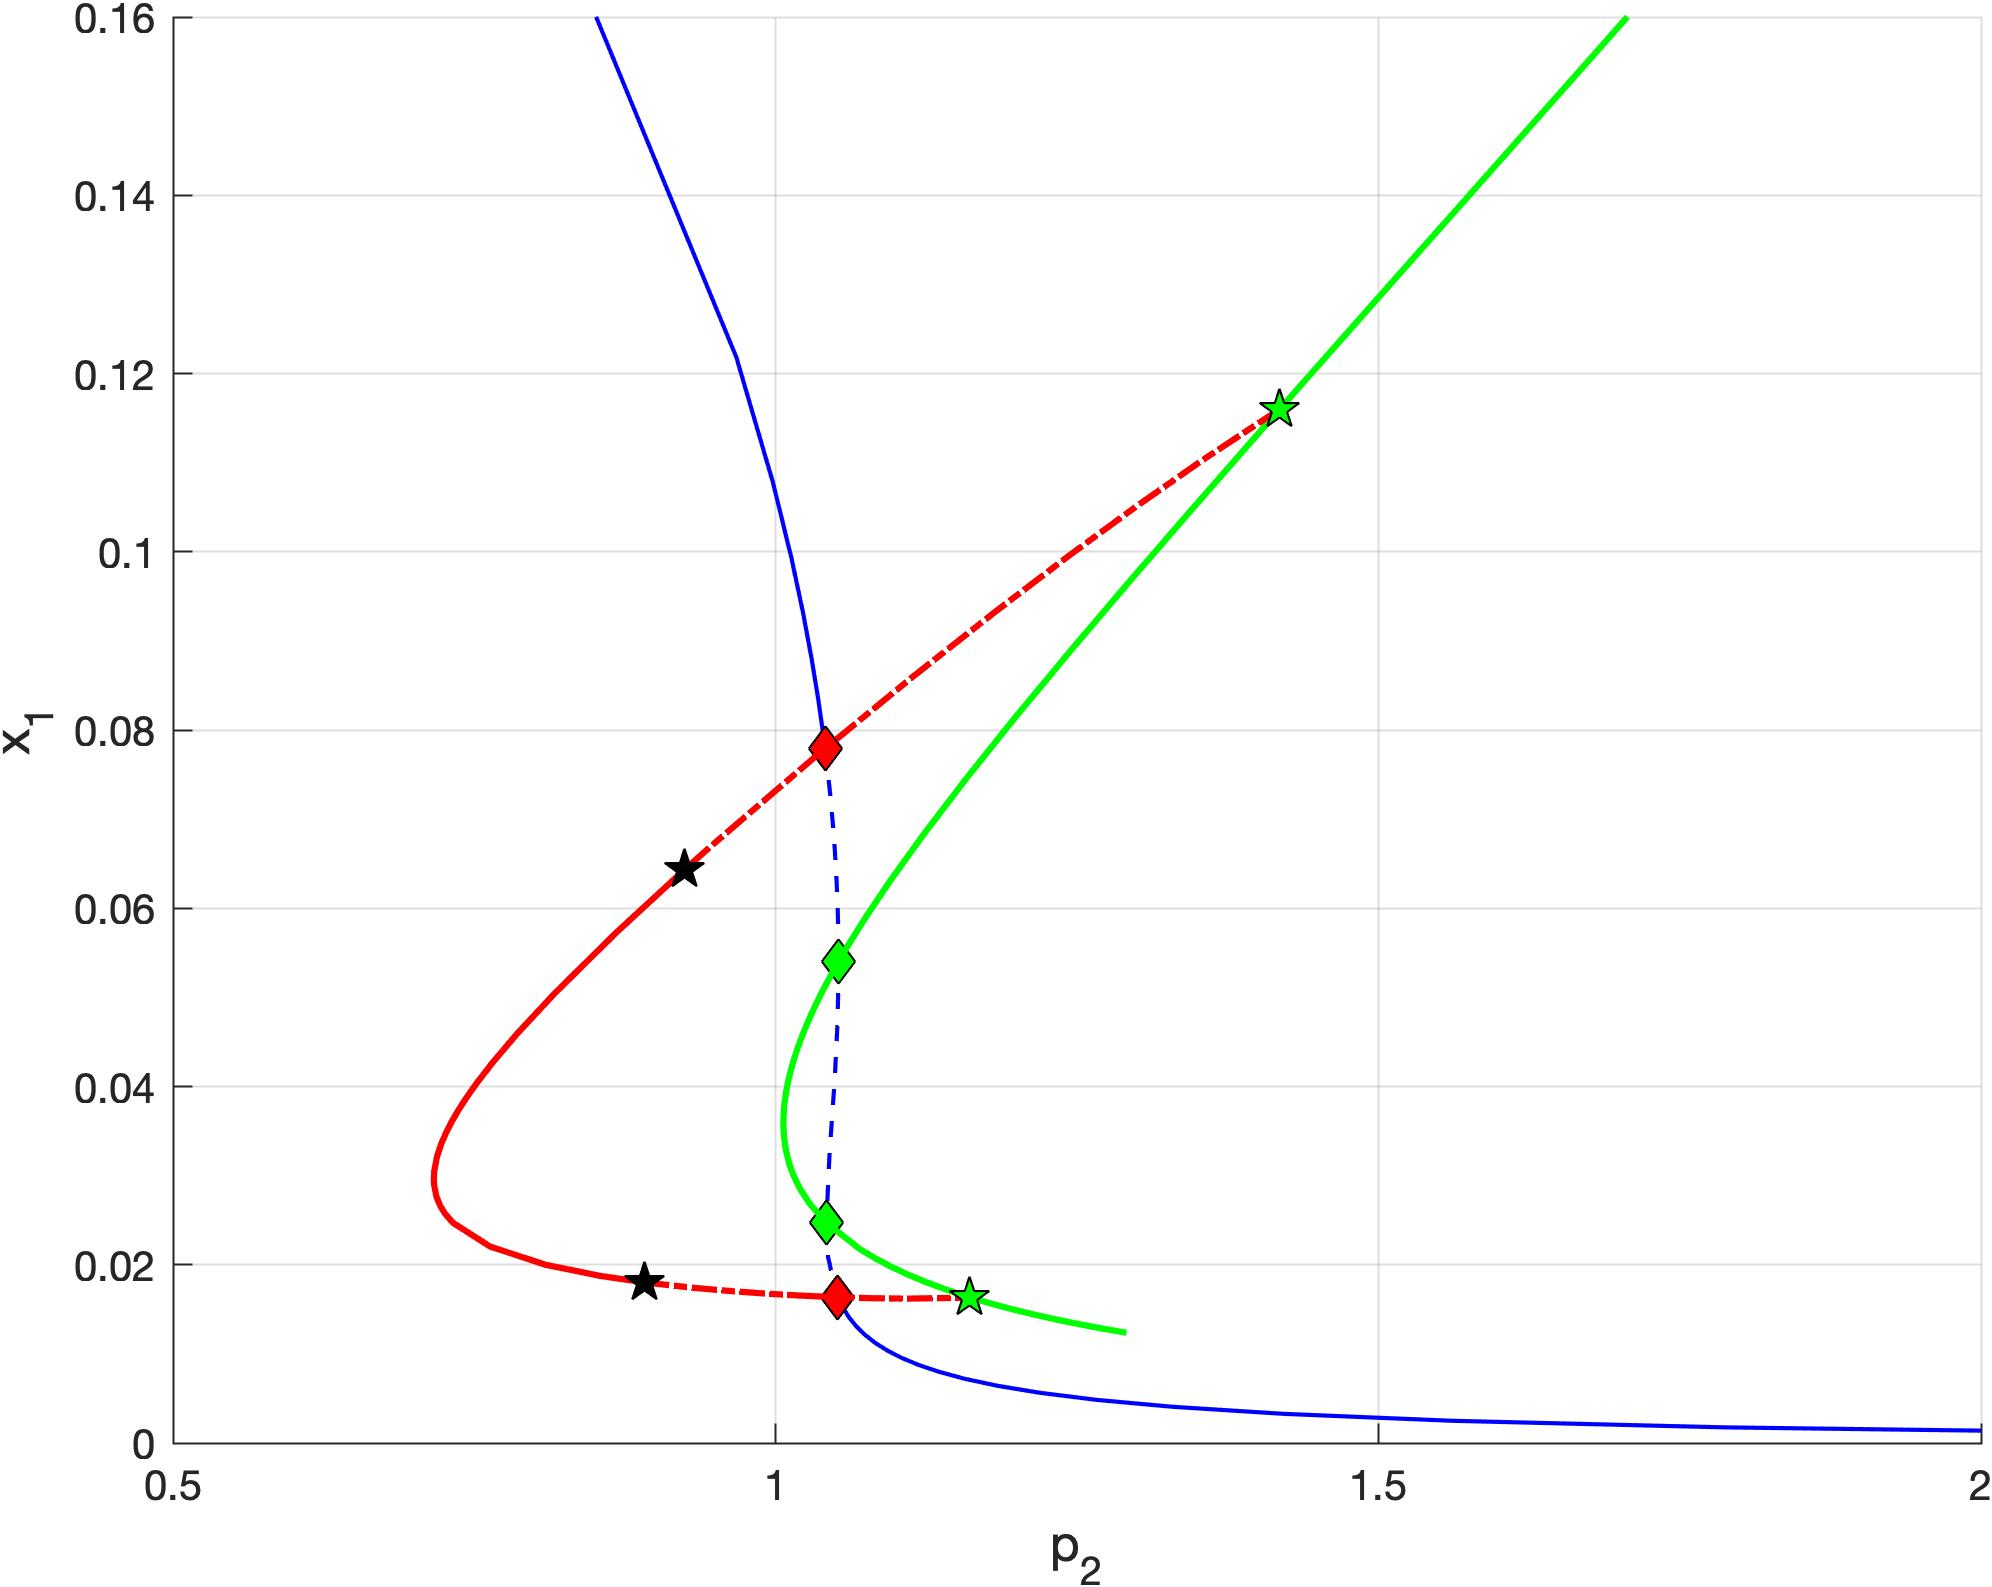
\includegraphics[width=4in]{Figures/Section7_2_1.jpg}
\caption{Families of equilibria (blue), saddle-node bifurcations of equilibria (green), and Hopf bifurcations of equilibria (red) for the vector field in Section~\ref{sec: Monitoring properties of equilibria}. The Hopf bifurcation curve terminates at each end on the saddle-node bifurcation curve at a Bogdanov-Takens points (green star) and consists of both subcritical (dash-dotted) and supercritical (solid) bifurcations, separated by generalized Hopf bifurcations (black stars). While the location of the latter is accurate to within tolerance, the change in the sign of the Lyapunov coefficient is not detected until beyond this point, as evidenced by the crossing of the top-most generalized Hopf bifurcation by the dash-dotted curve.}
\label{fig: Section7_2_1}
\end{figure}

You can continue along a curve of generalized Hopf bifurcations by embedding the \mcode{lyapunov} function as an \mcode{'inactive'} monitor function and fixing its value to $0$, as shown below. Since a generalized Hopf bifurcation is a co-dimension-two point, three parameters are allowed to vary along this curve.
\begin{lstlisting}[language=coco-highlight,frame=lines]
>> labs = coco_bd_labs('HB-curve', 'GH');
>> prob = coco_prob;
>> prob = ode_HB2HB(prob, '', 'HB-curve', labs(1));
>> data = struct('dfdxhan', F('x'), 'Dfdxdxhan', F({'x*v','x*v'}), ...
     'Dfdxdxdxhan', F({'x*v','x*v','x*v'}), 'nanflag', 1);
>> prob = ep_HB_add_func(prob, '', 'lyap', @lyapunov, data, ...
     'inactive', 'L1');
>> prob = coco_set_parival(prob, 'L1', 0);
>> prob = coco_set(prob, 'cont', 'PtMX', 50);
>> coco(prob, 'GH-curve', [], {'p2' 'p7' 'p1'}, {[0.4 3], [0 8]});

    STEP   DAMPING               NORMS              COMPUTATION TIMES
  IT SIT     GAMMA     ||d||     ||f||     ||U||   F(x)  DF(x)  SOLVE
   0                          3.52e-07  1.08e+01    0.0    0.0    0.0

 STEP    ...   LABEL  TYPE            p2           p7           p1
    0    ...       1  EP      9.2427e-01   3.0587e-01   2.5001e+00
   10    ...       2          8.9383e-01   3.2573e-01   2.3080e+00
   20    ...       3          8.7535e-01   3.3895e-01   2.1957e+00
   30    ...       4          8.5733e-01   3.5279e-01   2.0892e+00
   40    ...       5          8.3976e-01   3.6731e-01   1.9884e+00
   50    ...       6  EP      8.2262e-01   3.8254e-01   1.8928e+00

 STEP    ...   LABEL  TYPE            p2           p7           p1
    0    ...       7  EP      9.2427e-01   3.0587e-01   2.5001e+00
   10    ...       8          9.5437e-01   2.8827e-01   2.6987e+00
   20    ...       9          9.7499e-01   2.7722e-01   2.8399e+00
   30    ...      10          9.9613e-01   2.6666e-01   2.9890e+00
   40    ...      11          1.0178e+00   2.5655e-01   3.1463e+00
   50    ...      12  EP      1.0400e+00   2.4687e-01   3.3125e+00
\end{lstlisting}
Alternatively, embed the \mcode{lyapunov} function in the continuation problem as a \textit{zero function}, as in the following:
\begin{lstlisting}[language=coco-highlight,frame=lines]
>> labs = coco_bd_labs('HB-curve', 'GH');
>> prob = coco_prob;
>> prob = ode_HB2HB(prob, '', 'HB-curve', labs(2));
>> data = struct('dfdxhan', F('x'), 'Dfdxdxhan', F({'x*v','x*v'}), ...
     'Dfdxdxdxhan', F({'x*v','x*v','x*v'}), 'nanflag', 1);
>> prob = ep_HB_add_func(prob, '', 'lyap', @lyapunov, data, 'zero');
>> prob = coco_set(prob, 'cont', 'PtMX', 50);
>> coco(prob, 'GH-curve', [], {'p2' 'p7' 'p1'}, {[0.4 3], [0 8]});

    STEP   DAMPING               NORMS              COMPUTATION TIMES
  IT SIT     GAMMA     ||d||     ||f||     ||U||   F(x)  DF(x)  SOLVE
   0                          1.30e-05  1.08e+01    0.0    0.0    0.0
   1   1  1.00e+00  5.25e-05  9.57e-07  1.08e+01    0.0    0.1    0.0
   2   1  1.00e+00  3.74e-10  1.75e-12  1.08e+01    0.0    0.2    0.0

 STEP    ...   LABEL  TYPE            p2           p7           p1
    0    ...       1  EP      8.9132e-01   2.3248e-01   2.5000e+00
   10    ...       2          8.6719e-01   2.4549e-01   2.3487e+00
   20    ...       3          8.5291e-01   2.5400e-01   2.2608e+00
   30    ...       4          8.3885e-01   2.6307e-01   2.1753e+00
   40    ...       5          8.2504e-01   2.7274e-01   2.0923e+00
   50    ...       6  EP      8.1150e-01   2.8305e-01   2.0121e+00

 STEP    ...   LABEL  TYPE            p2           p7           p1
    0    ...       7  EP      8.9132e-01   2.3248e-01   2.5000e+00
   10    ...       8          9.1572e-01   2.2083e-01   2.6564e+00
   20    ...       9          9.3067e-01   2.1432e-01   2.7539e+00
   30    ...      10          9.4573e-01   2.0819e-01   2.8535e+00
   40    ...      11          9.6089e-01   2.0240e-01   2.9550e+00
   50    ...      12  EP      9.7614e-01   1.9693e-01   3.0585e+00
\end{lstlisting}

\subsection{Monitoring properties of periodic orbits}
\label{sec: Monitoring properties of periodic orbits}

A similar construction as in Sec.~\ref{sec: Monitoring properties of equilibria} applies to the monitoring of properties of periodic orbits using the \mcode{po_add_bddat} constructor. Suppose, for example, that you want to monitor the Fourier integral
\[
\mathcal{I}_n=\frac{1}{T}\int_{-T/2}^{T/2}x(t)\exp{\left(-\mathrm{i}2n\pi t/T\right)}\,\mathrm{d}t
\]
for each member $x(t)$ of a family of periodic orbits of a vector field $f(x,p)$, associated period $T$, and some integer $n$. 

\textsc{coco} represents such an orbit in terms of a \textit{partition} of the interval $[-T/2,T/2]$ into $N$ possibly unequal intervals and, on each interval, a set of vectors at $m+1$ uniformly spaced instants of time, including the interval end points. The interval lengths are tracked by the sequence $\{\kappa_j\}_{j=1}^N$, such that the $j$-th interval extends from $t_j$ to $t_{j+1}=t_j+T\kappa_j/N$ and $\sum_{j=1}^N\kappa_j=N$. The $j$-th interval is associated with a predefined set of $m$ \textit{collocation nodes} $t_j+(1+z_i)T\kappa_j/2N$ with $z_i\in[-1,1]$ and associated \textit{quadrature weights} $T\kappa_jw_i/2N$, so that
\[
\mathcal{I}_n\approx \frac{1}{2N}\sum_{j=1}^N\kappa_j\sum_{i=1}^m w_ix(t_j+(1+z_i)T\kappa_j/2N)\exp{\left(-\mathrm{i}2n\pi (t_j+(1+z_i)T\kappa_j/2N)/T\right)}
\]
If $x(t)$ is approximated by an $m$-th order polynomial on the $j$-th interval, then the values $x(t_j+(1+z_i)T\kappa_j/2N)$ may be obtained from predefined linear combinations of the values of $x(t)$ at the $m+1$ uniformly spaced instants of time on that interval.

The function \mcode{fourier} below uses the fields of the \mcode{data} argument to compute this double-sum approximation of the Fourier integral.
\begin{lstlisting}[language=coco-highlight,frame=shadowbox]
function y = fourier(data, xbp, T0, T, p)

mps = data.coll_seg.maps;
msh = data.coll_seg.mesh;
xcn = reshape(mps.W*xbp, mps.x_shp);
ecn = exp(-2i*data.n*pi*msh.tcn);
y   = (msh.fka.*msh.fwt.*xcn)*ecn/2/mps.NTST;

end
\end{lstlisting}
Here, \mcode{xcn} and \mcode{ecn} contain a rectangular array with columns given by $x(t_j+(1+z_i)T\kappa_j/2N)$ and a column array  with entries given by $\exp{\left(-\mathrm{i}2n\pi (t_j+(1+z_i)T\kappa_j/2N)/T\right)}$, respectively, for $j=1,\ldots,N$, $i=1,\ldots,m$. A verification of this encoding is given by the following application to the family of periodic orbits emanating from a subcritical Hopf bifurcation, as well as the corresponding curve of saddle-node bifurcations of periodic orbits computed in Sec.~\ref{sec: Continuing from Hopf bifurcations}.
\begin{lstlisting}[language=coco-highlight,frame=lines]
>> syms r2 x1 x2 p1 p2
>> r2 = x1^2+x2^2;
>> F = sco_sym2funcs(...
     [x1*(p1+p2*r2-r2^2)-x2; x2*(p1+p2*r2-r2^2)+x1], ...
     {[x1; x2], [p1; p2]}, {'x', 'p'}, 'filename', 'sys_hopf');
>> f = struct('f', F(''), 'dfdx', F('x'), 'dfdp', F('p'), ...
     'dfdx_dx', F('x*v'), 'dfdxdx_dx', F({'x','x*v'}), ...
     'dfdpdx_dx', F({'p','x*v'}));
>> prob = coco_prob;
>> prob = ode_isol2ep(prob, '', f, [0; 0], {'p1', 'p2'}, [-1; 1]);
>> coco(prob, 'ep_run', [], 'p1', [-1 1]);

    STEP   DAMPING               NORMS              COMPUTATION TIMES
  IT SIT     GAMMA     ||d||     ||f||     ||U||   F(x)  DF(x)  SOLVE
   0                          0.00e+00  1.73e+00    0.0    0.0    0.0

 STEP      TIME        ||U||  LABEL  TYPE            p1
    0  00:00:00   1.7321e+00      1  EP     -1.0000e+00
    5  00:00:00   1.0000e+00      2  HB      1.5899e-07
    8  00:00:00   1.7321e+00      3  EP      1.0000e+00
    
>> HB = coco_bd_labs('ep_run', 'HB');
>> prob = coco_prob;
>> prob = ode_HB2po(prob, '', 'ep_run', HB);
>> prob = coco_set(prob, 'cont', 'PtMX', [50 0]);
>> prob = po_add_bddat(prob, '', 'cx1', @fourier, 'data', struct('n', 1));
>> coco(prob, 'po_run', [], {'p1' 'po.period'}, [-1 1]);

    STEP   DAMPING               NORMS              COMPUTATION TIMES
  IT SIT     GAMMA     ||d||     ||f||     ||U||   F(x)  DF(x)  SOLVE
   0                          6.75e-06  8.94e+00    0.0    0.0    0.0
   1   1  1.00e+00  1.96e-06  2.68e-13  8.94e+00    0.0    0.0    0.0
   2   1  1.00e+00  1.14e-12  2.84e-18  8.94e+00    0.0    0.0    0.0

 STEP    ...   LABEL  TYPE            p1           p2         cx1
    0    ...       1  EP     -9.9933e-07   1.0000e+00  4.9983e-04
   10    ...       2         -2.2549e-01   1.0000e+00  2.9302e-01
   12    ...       3  FP     -2.5000e-01   1.0000e+00  3.5355e-01
   12    ...       4  SN     -2.5000e-01   1.0000e+00  3.5355e-01
   20    ...       5          4.9782e-01   1.0000e+00  5.8412e-01
   23    ...       6  EP      1.0000e+00   1.0000e+00  6.3601e-01
   
>> SN = coco_bd_labs('po_run', 'SN');
>> prob = coco_prob;
>> prob = ode_po2SN(prob, '', 'po_run', SN(1));
>> prob = po_add_bddat(prob, '', 'cx1', @fourier, 'data', struct('n', 1));
>> coco(prob, 'po_SN_run', [], {'p1', 'p2'}, {[-1 1] [0.001 3]});

    STEP   DAMPING               NORMS              COMPUTATION TIMES
  IT SIT     GAMMA     ||d||     ||f||     ||U||   F(x)  DF(x)  SOLVE
   0                          1.21e-05  1.25e+01    0.0    0.0    0.0
   1   1  1.00e+00  4.97e-05  2.06e-11  1.25e+01    0.0    0.0    0.0
   2   1  1.00e+00  9.84e-11  3.19e-15  1.25e+01    0.0    0.0    0.0

 STEP    ...   LABEL  TYPE            p1           p2         cx1
    0    ...       1  EP     -2.5000e-01   1.0000e+00  3.5355e-01
    8    ...       2  EP     -1.0000e+00   2.0000e+00  5.0000e-01

 STEP    ...   LABEL  TYPE            p1           p2         cx1
    0    ...       3  EP     -2.5000e-01   1.0000e+00  3.5355e-01
   10    ...       4         -6.3961e-04   5.0581e-02  7.9515e-02
   12    ...       5  EP     -2.5000e-07   1.0000e-03  1.1180e-02
\end{lstlisting}
Since $x_1(t)$ is known to equal $r\cos{t}$, we compute $r$ as twice the real part of the Fourier coefficient for $n=1$. In the visualization generated by the following commands (cf.\ Fig.~\ref{fig: Section7_3_1}), the results of the computation are compared to the predicted relationships $p_1=r^4-p_2r^2$ along the family of periodic orbits and $p_1=-r^4,\,p_2=2r^2$ along the family of saddle-node bifurcations.
\begin{lstlisting}[language=coco-highlight,frame=lines]
>> figure(1)
>> clf
>> hold on
>> coco_plot_bd('po_run', 'p1', 'p2', 'cx1', @(x) 2*real(x(1,:)))
>> thm = struct();
>> thm.lspec = {{'ro', 'MarkerFaceColor', 'r'}, {'ro'}};
>> coco_plot_bd(thm, 'po_run', ...
     {'cx1', 'p2'}, @(x,y) (2*real(x(1,:))).^4-y.*(2*real(x(1,:))).^2, ...
     'p2', 'cx1', @(x) 2*real(x(1,:)));
>> coco_plot_bd('po_SN_run', 'p1', 'p2', 'cx1', @(x) 2*real(x(1,:)))
>> thm.lspec = {'ko', 'MarkerFaceColor', 'k'};
>> thm.xlab = 'p1';
>> thm.ylab = 'p2';
>> thm.zlab = 'r';
>> coco_plot_bd(thm, 'po_SN_run', ...
     'cx1', @(x) -(2*real(x(1,:))).^4, ...
     'cx1', @(x) 2*(2*real(x(1,:))).^2, ...
     'cx1', @(x) 2*real(x(1,:)));
>> hold off
>> grid on
>> view(3)
\end{lstlisting}
\begin{figure}[h]
\centering
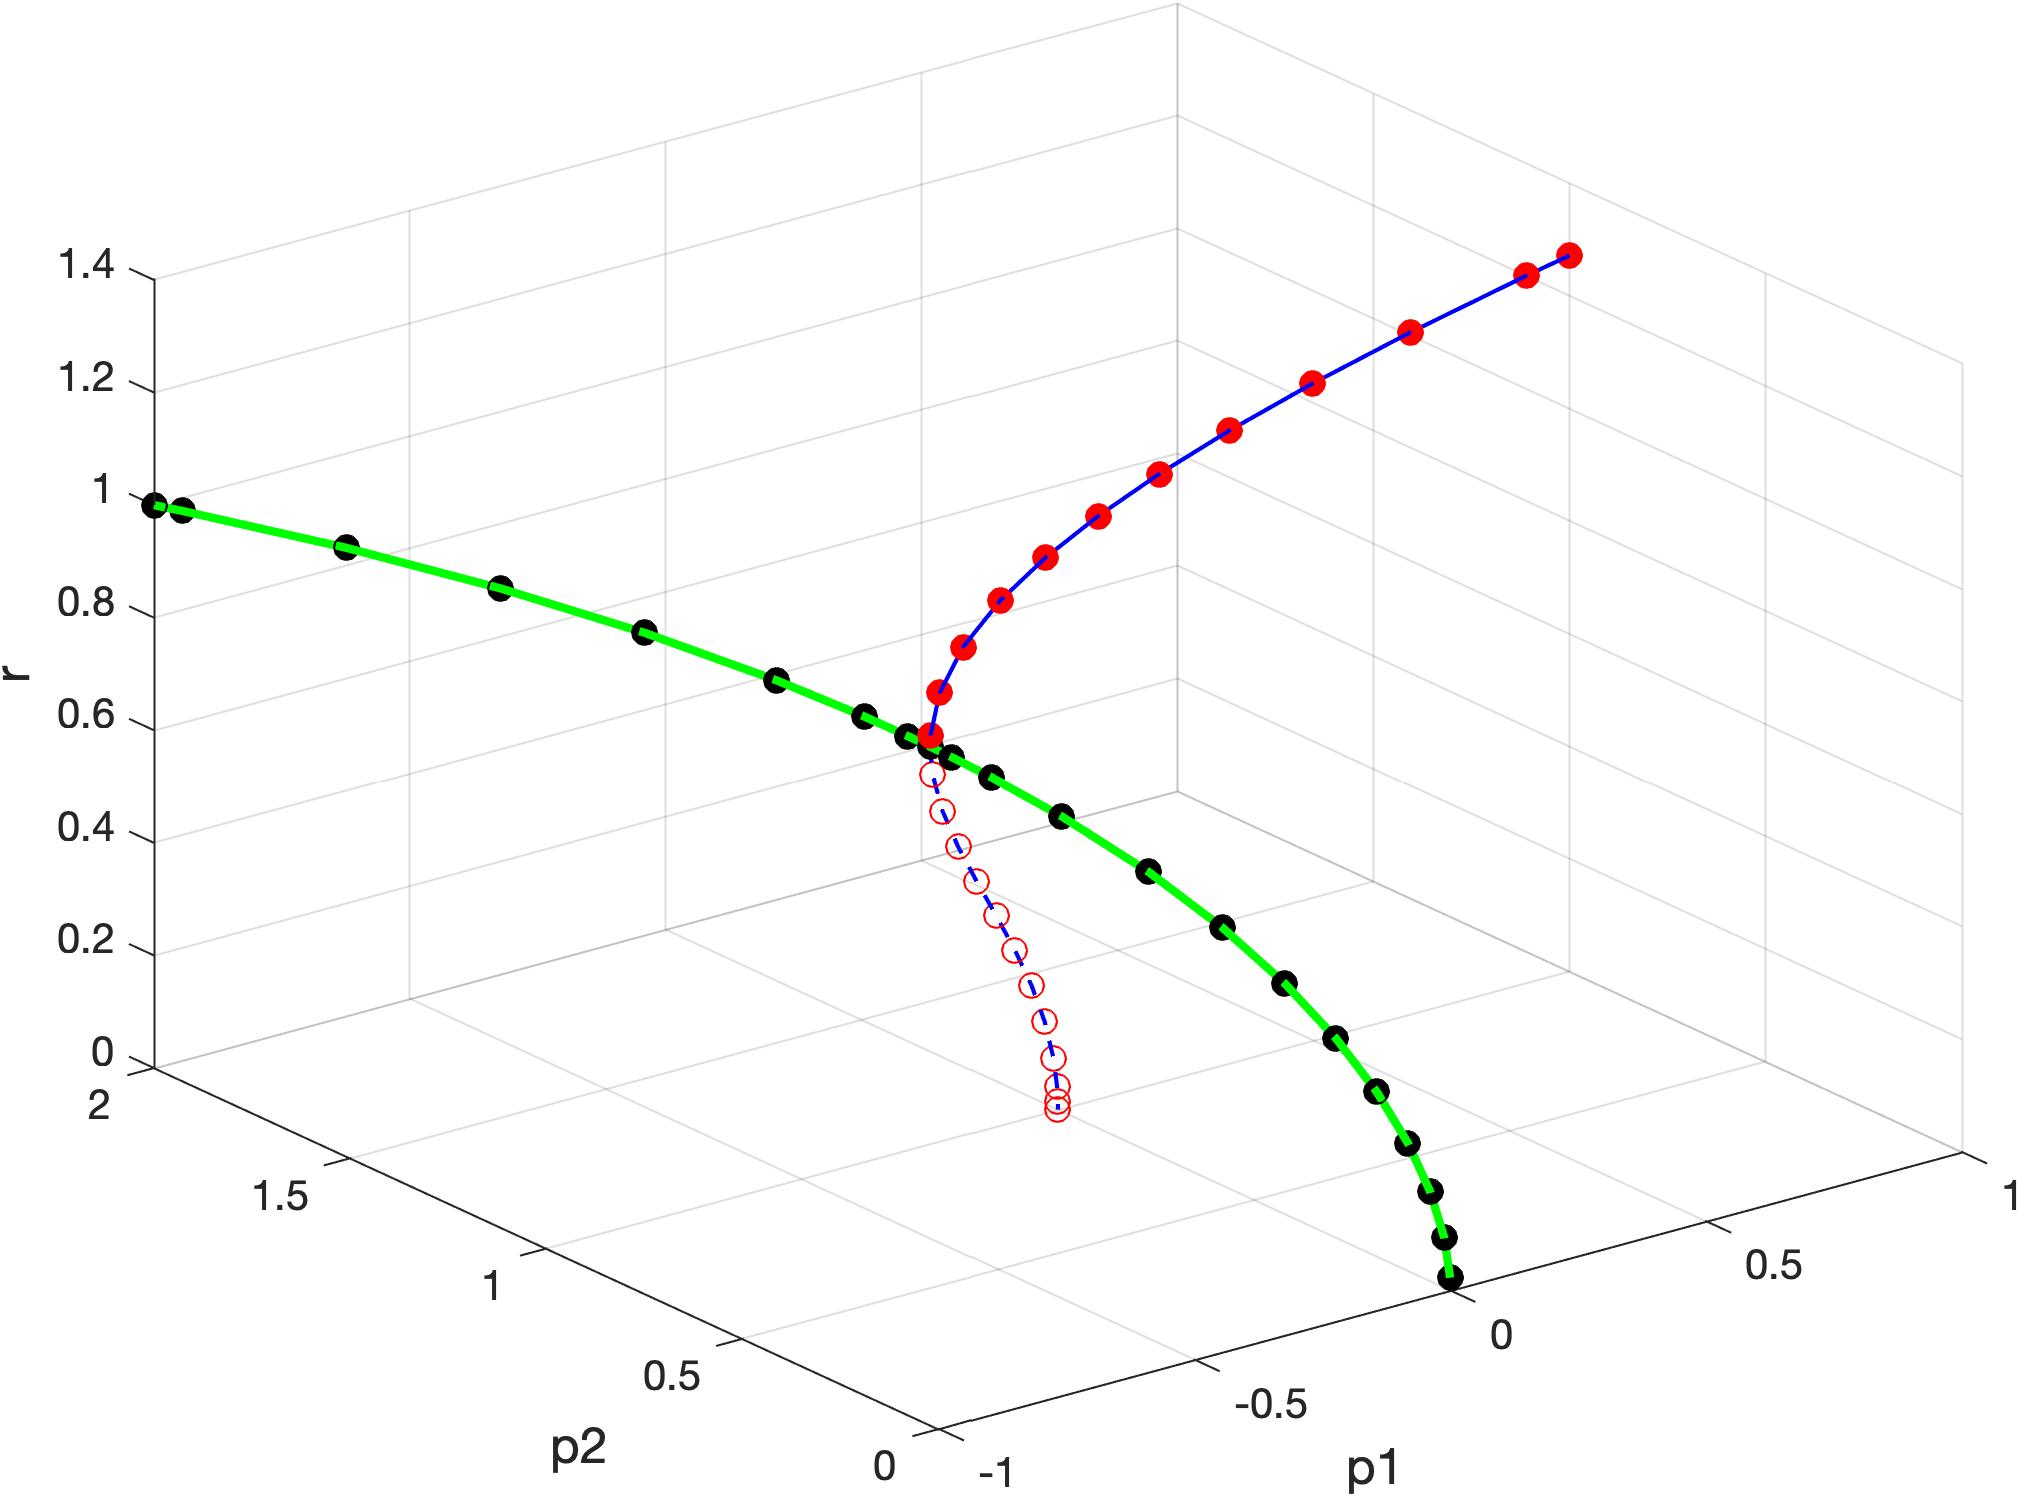
\includegraphics[width=4in]{Figures/Section7_3_1.jpg}
\caption{Comparison between theoretical predictions (red and black balls) and the results of continuation along families of periodic orbits (blue solid) and saddle-node bifurcations of periodic orbits (green solid) associated with the Hopf normal form in Sec.~\ref{sec: Continuing from Hopf bifurcations}. The vertical coordinate $r$ represents the projection onto the Fourier coefficient associated with $\cos t$.}
\label{fig: Section7_3_1}
\end{figure}

\subsection{Tracking and constraining orbit maxima}
\label{sec: Tracking and constraining orbit maxima}

The \mcode{po_add_func} constructor mirrors the functionality of \mcode{ep_add_func} by allowing you to monitor properties of periodic orbits during continuation, automatically detect special points associated with particular numerical thresholds, and impose constraints on such properties.

To illustrate this functionality, suppose that you have performed continuation along a family of equilibria, including detection of a Hopf bifurcation, as shown in the following sequence of commands.
\begin{lstlisting}[language=coco-highlight,frame=lines]
>> syms x1 x2 x3 p1 p2
>> F = sco_sym2funcs(...
     [p1*x1+x2+p2*x1^2; -x1+p1*x2+x2*x3; (p1^2-1)*x2-x1-x3+x1^2], ...
     {[x1; x2; x3], [p1; p2]}, {'x', 'p'}, 'filename', 'sys_marsden');
>> f = struct('f', F(''), 'dx', F('x'), 'dp', F('p'));
>> prob = coco_prob;
>> prob = ode_isol2ep(prob, '', f, [0; 0; 0], {'p1', 'p2'}, [-1; 6]);
>> coco(prob, 'ep_run', [], 'p1', [-1 1]);

    STEP   DAMPING               NORMS              COMPUTATION TIMES
  IT SIT     GAMMA     ||d||     ||f||     ||U||   F(x)  DF(x)  SOLVE
   0                          0.00e+00  6.16e+00    0.0    0.0    0.0

 STEP      TIME        ||U||  LABEL  TYPE            p1
    0  00:00:00   6.1644e+00      1  EP     -1.0000e+00
    5  00:00:00   6.0000e+00      2  HB      1.5899e-07
    8  00:00:00   6.1644e+00      3  EP      1.0000e+00
\end{lstlisting}
You then proceed to continue along a family of periodic orbits emanating from the Hopf bifurcation as shown below.
\begin{lstlisting}[language=coco-highlight,frame=lines]
>> HB = coco_bd_labs('ep_run', 'HB');
>> prob = coco_prob;
>> prob = ode_HB2po(prob, '', 'ep_run', HB);
>> prob = coco_set(prob, 'cont', 'PtMX', [50 0], 'NAdapt', 1);
>> coco(prob, 'po_run', [], {'p1' 'po.period'}, [-1 1]);

    STEP   DAMPING               NORMS              COMPUTATION TIMES
  IT SIT     GAMMA     ||d||     ||f||     ||U||   F(x)  DF(x)  SOLVE
   0                          7.39e-06  1.07e+01    0.0    0.0    0.0
   1   1  1.00e+00  3.53e-05  9.58e-12  1.07e+01    0.0    0.0    0.0
   2   1  1.00e+00  2.48e-10  5.00e-18  1.07e+01    0.0    0.0    0.0

 STEP      TIME        ||U||  LABEL  TYPE            p1    po.period
    0  00:00:00   1.0722e+01      1  EP     -7.8687e-07   6.2832e+00
   10  00:00:00   1.0975e+01      2         -6.5370e-03   6.4878e+00
   18  00:00:01   1.2676e+01      3  SN     -2.0251e-02   7.7362e+00
   18  00:00:01   1.2676e+01      4  FP     -2.0252e-02   7.7365e+00
   20  00:00:02   1.3777e+01      5         -1.8542e-02   8.5358e+00
   30  00:00:02   1.8325e+01      6         -1.3582e-02   1.1805e+01
   40  00:00:03   2.3076e+01      7         -1.3193e-02   1.5189e+01
   50  00:00:04   2.7721e+01      8  EP     -1.3160e-02   1.8625e+01
\end{lstlisting}
By executing the command
\begin{lstlisting}[language=coco-highlight,frame=lines]
>> coco_plot_sol('po_run', '', 't', 'x')
\end{lstlisting}
you note from the visualization (cf.\ Fig.~\ref{fig: Section7_4_1}) that the periodic function associated with label \mcode{5} achieves a maximum in $x_1$ near $t=5.17$. 
\begin{figure}[h]
\centering
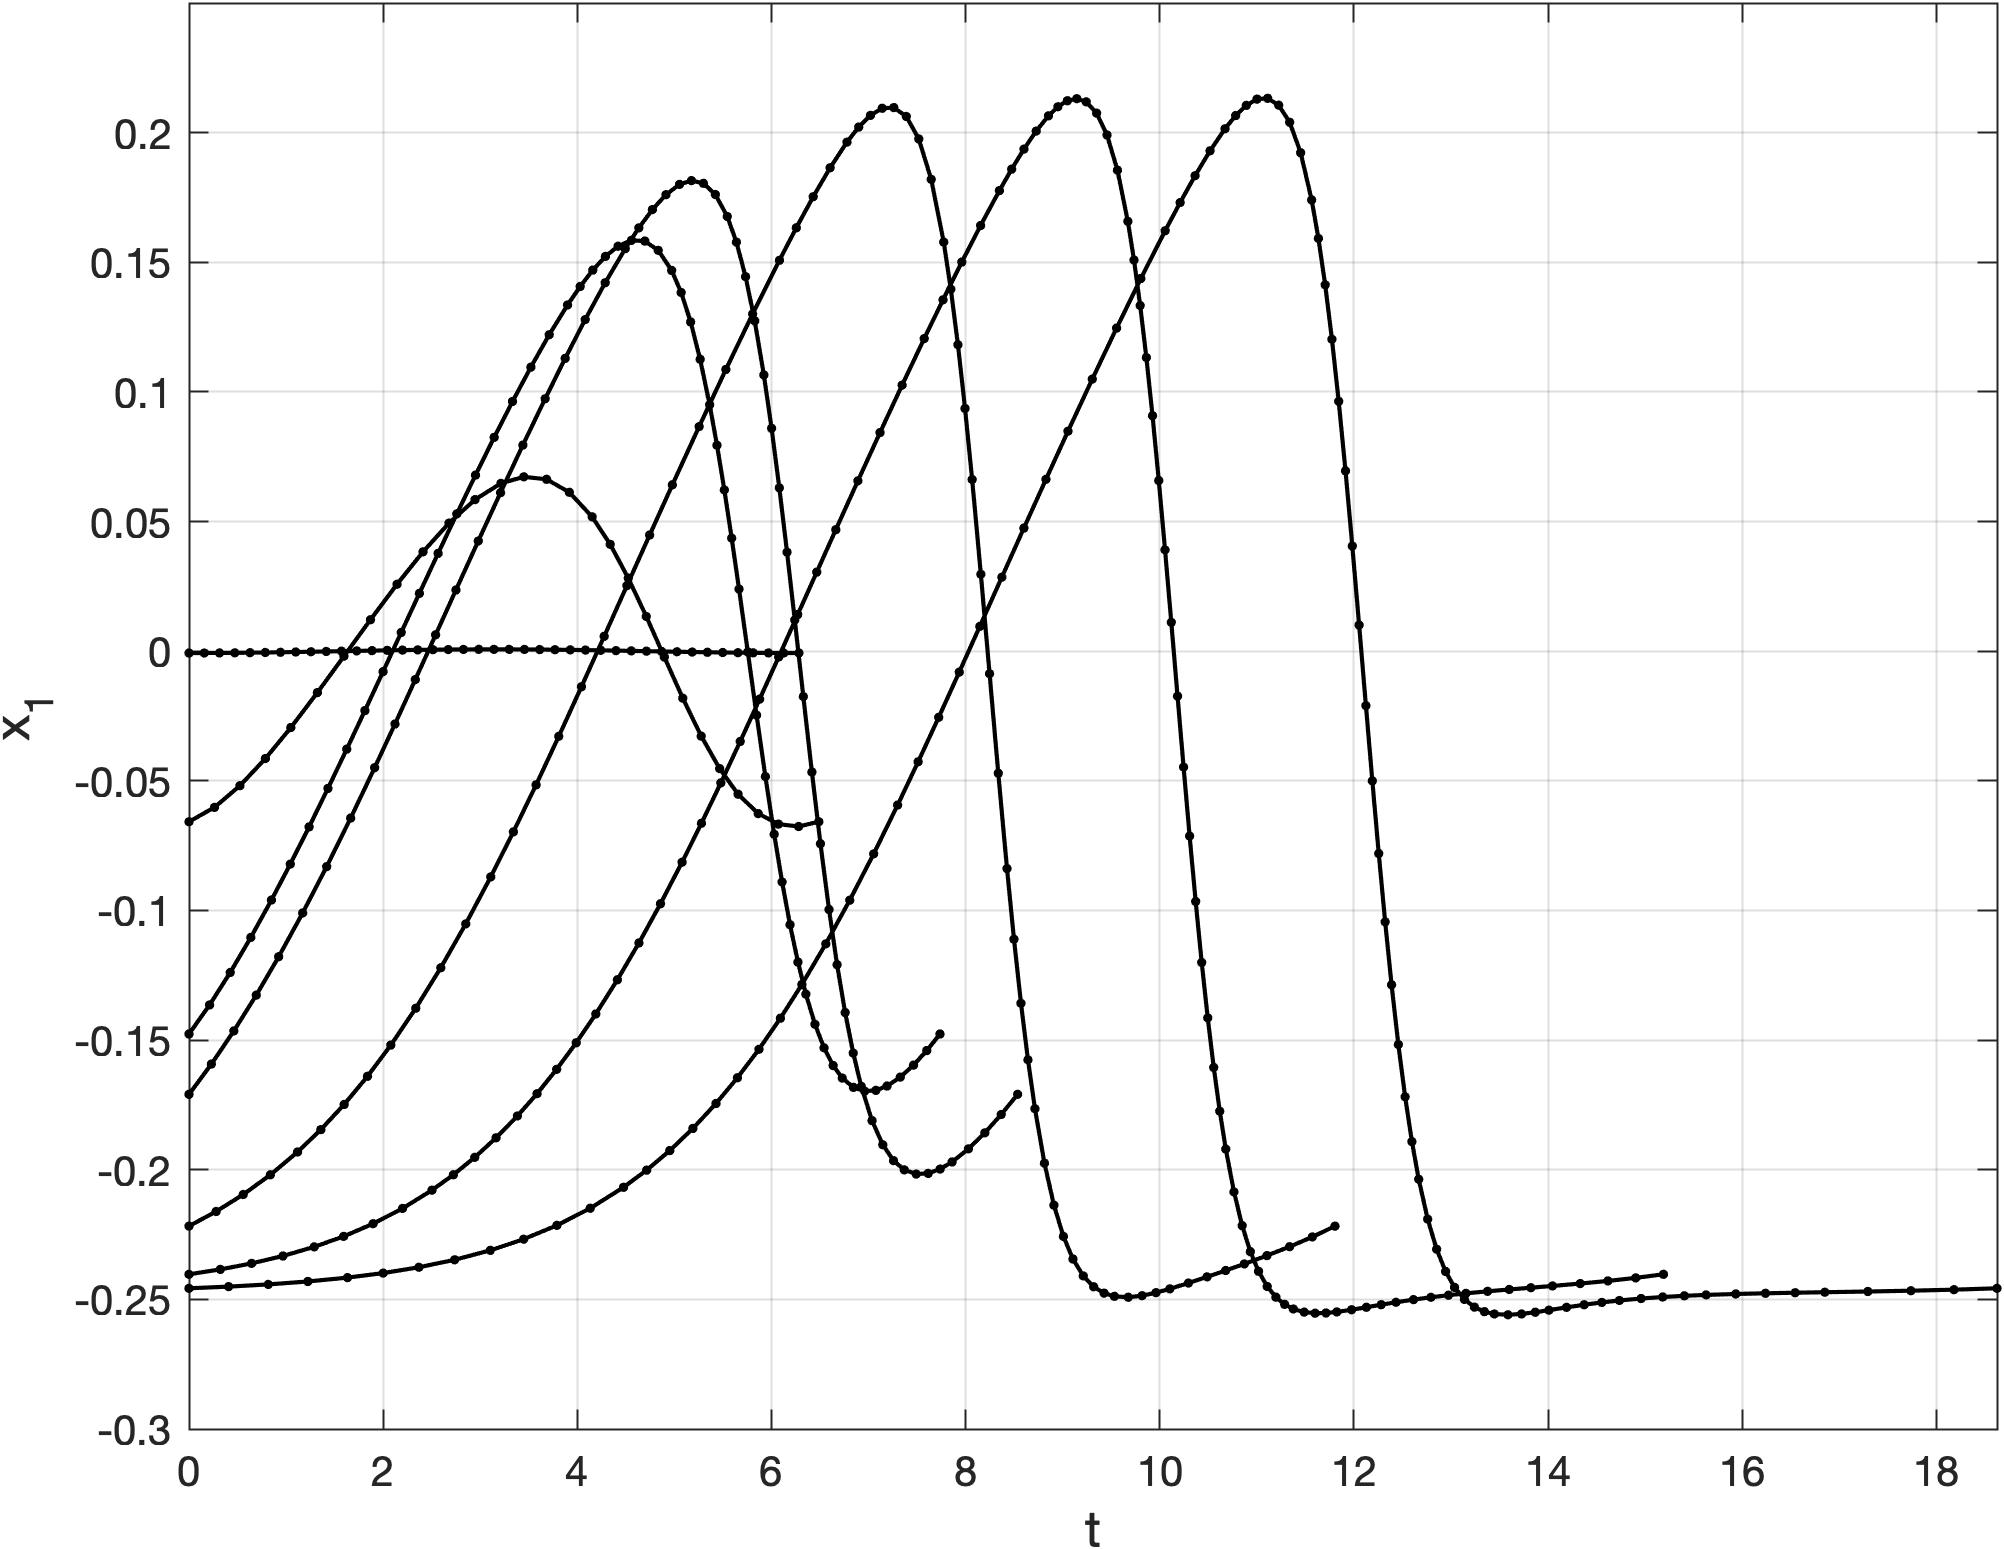
\includegraphics[width=4in]{Figures/Section7_4_1.jpg}
\caption{Time histories for labeled periodic orbits found during continuation using the code in Sect.~\ref{sec: Tracking and constraining orbit maxima}.}
\label{fig: Section7_4_1}
\end{figure}

It now occurs to you that it could be interesting to track the maximum value of $x_1$ along the family of periodic orbits. To this end, you define the function  \mcode{slope} shown below.
\begin{lstlisting}[language=coco-highlight,frame=shadowbox]
function y = slope(data, xbp, T0, T, p, t)

m    = data.coll_seg.int.NCOL;
xdim = data.coll_seg.int.dim;
N    = data.coll_seg.maps.NTST;
tmi  = data.coll_seg.mesh.tmi;
tbp  = data.coll_seg.mesh.tbp;

% find interval
trs    = (t-T0)/T;
J = min(N, find(N*trs>=tmi, 1, 'last'));
xbpint = xbp((J-1)*xdim*(m+1)+(1:xdim*(m+1)));
tint   = tbp((J-1)*(m+1)+(1:m+1));
ts     = linspace(-1, 1, m+1)';

% interpolated point
s  = repmat(2*(trs-tint(1))/(tint(end)-tint(1))-1, [1 m+1 m+1]);
sj = repmat(reshape(ts, [1 m+1 1]), [1 1 m+1]);
sk = repmat(reshape(ts, [1 1 m+1]), [1 m+1 1]);

t1 = s-sk;
t2 = sj-sk;
idx = find(abs(t2)<=eps);
t1(idx) = 1;
t2(idx) = 1;

x = kron(prod(t1./t2, 3), eye(xdim))*xbpint;

% interpolated derivative
s  = repmat(2*(trs-tint(1))/(tint(end)-tint(1))-1, [1 m+1 m+1 m+1]);
sj = repmat(reshape(ts, [1 m+1 1 1]), [1 1 m+1 m+1]);
sk = repmat(reshape(ts, [1 1 m+1 1]), [1 m+1 1 m+1]);
sl = repmat(reshape(ts, [1 1 1 m+1]), [1 m+1 m+1 1]);

t3 = sj(:,:,:,1)-sk(:,:,:,1);
t4 = s-sl;
t5 = sj-sl;
idx1 = find(abs(t5)<=eps);
idx2 = find(abs(t3)<=eps);
idx3 = find(abs(sk-sl)<=eps);
t5(union(idx1, idx3)) = 1;
t4(union(idx1, idx3)) = 1;
t3(idx2) = 1;
t3       = 1.0./t3;
t3(idx2) = 0;

xt = kron(sum(t3.*prod(t4./t5, 4), 3), eye(xdim))*xbpint;

y = [t; x(data.idx); xt(data.idx)];

end
\end{lstlisting}
This uses Lagrange interpolation (as described in Section 6.2.2 of \textit{Recipes for Continuation}) to compute numerical values for a component of the state and the corresponding time derivative at a given instant of time and returns all three of these quantities in the output argument. The function is introduced to the continuation problem in the sequence of commands shown below, where the time instant is held fixed at $5.17$, while $x_1(5.17)$ and $\dot{x}_1(5.17)$ vary.
\begin{lstlisting}[language=coco-highlight,frame=lines]
>> prob = coco_prob;
>> prob = ode_po2po(prob, '', 'po_run', 5);
>> prob = coco_set(prob, 'cont', 'PtMX', [0 50], 'NAdapt', 1);
>> prob = po_add_func(prob, '', 'max', @slope, struct('idx', 1), ...
     {'trs', 'xrs', 'xtrs'}, 'inactive', 'u0', 5.17);
>> coco(prob, 'new_po_run1', [], {'p1' 'po.period', 'xrs', 'xtrs'}, [-1 1]);

    STEP   DAMPING               NORMS              COMPUTATION TIMES
  IT SIT     GAMMA     ||d||     ||f||     ||U||   F(x)  DF(x)  SOLVE
   0                          2.01e-15  1.47e+01    0.0    0.0    0.0

 STEP    ...   LABEL  TYPE            p1    po.period          xrs         xtrs
    0    ...       1  EP     -1.8542e-02   8.5358e+00   1.8148e-01   9.0100e-04
   10    ...       2         -1.3822e-02   1.1232e+01   1.0514e-01   4.1433e-02
   20    ...       3         -1.3211e-02   1.4606e+01  -4.9327e-02   3.0655e-02
   30    ...       4         -1.3161e-02   1.8032e+01  -1.7123e-01   2.0405e-02
   40    ...       5         -1.3157e-02   2.1499e+01  -2.2523e-01   1.2060e-02
   47    ...       6  SN     -1.3156e-02   2.3711e+01  -2.3799e-01   5.3241e-03
   50    ...       7  EP     -1.3156e-02   2.4987e+01  -2.4176e-01   3.3737e-03
\end{lstlisting}
The results of the computation are visualized using the following commands (cf.\ Fig.~\ref{fig: Section7_4_2}).
\begin{lstlisting}[language=coco-highlight,frame=lines]
>> figure(1)
>> clf
>> hold on
>> coco_plot_sol('new_po_run1', '', 't', 'x')
>> tx = coco_bd_vals('new_po_run1', 'all', {'trs', 'xrs'});
>> plot(tx(1,:), tx(2,:), 'ro', 'MarkerFaceColor', 'r');
>> hold off
>> grid on
>> box on
>> axis([0 inf -0.3 0.25])
\end{lstlisting}
\begin{figure}[h]
\centering
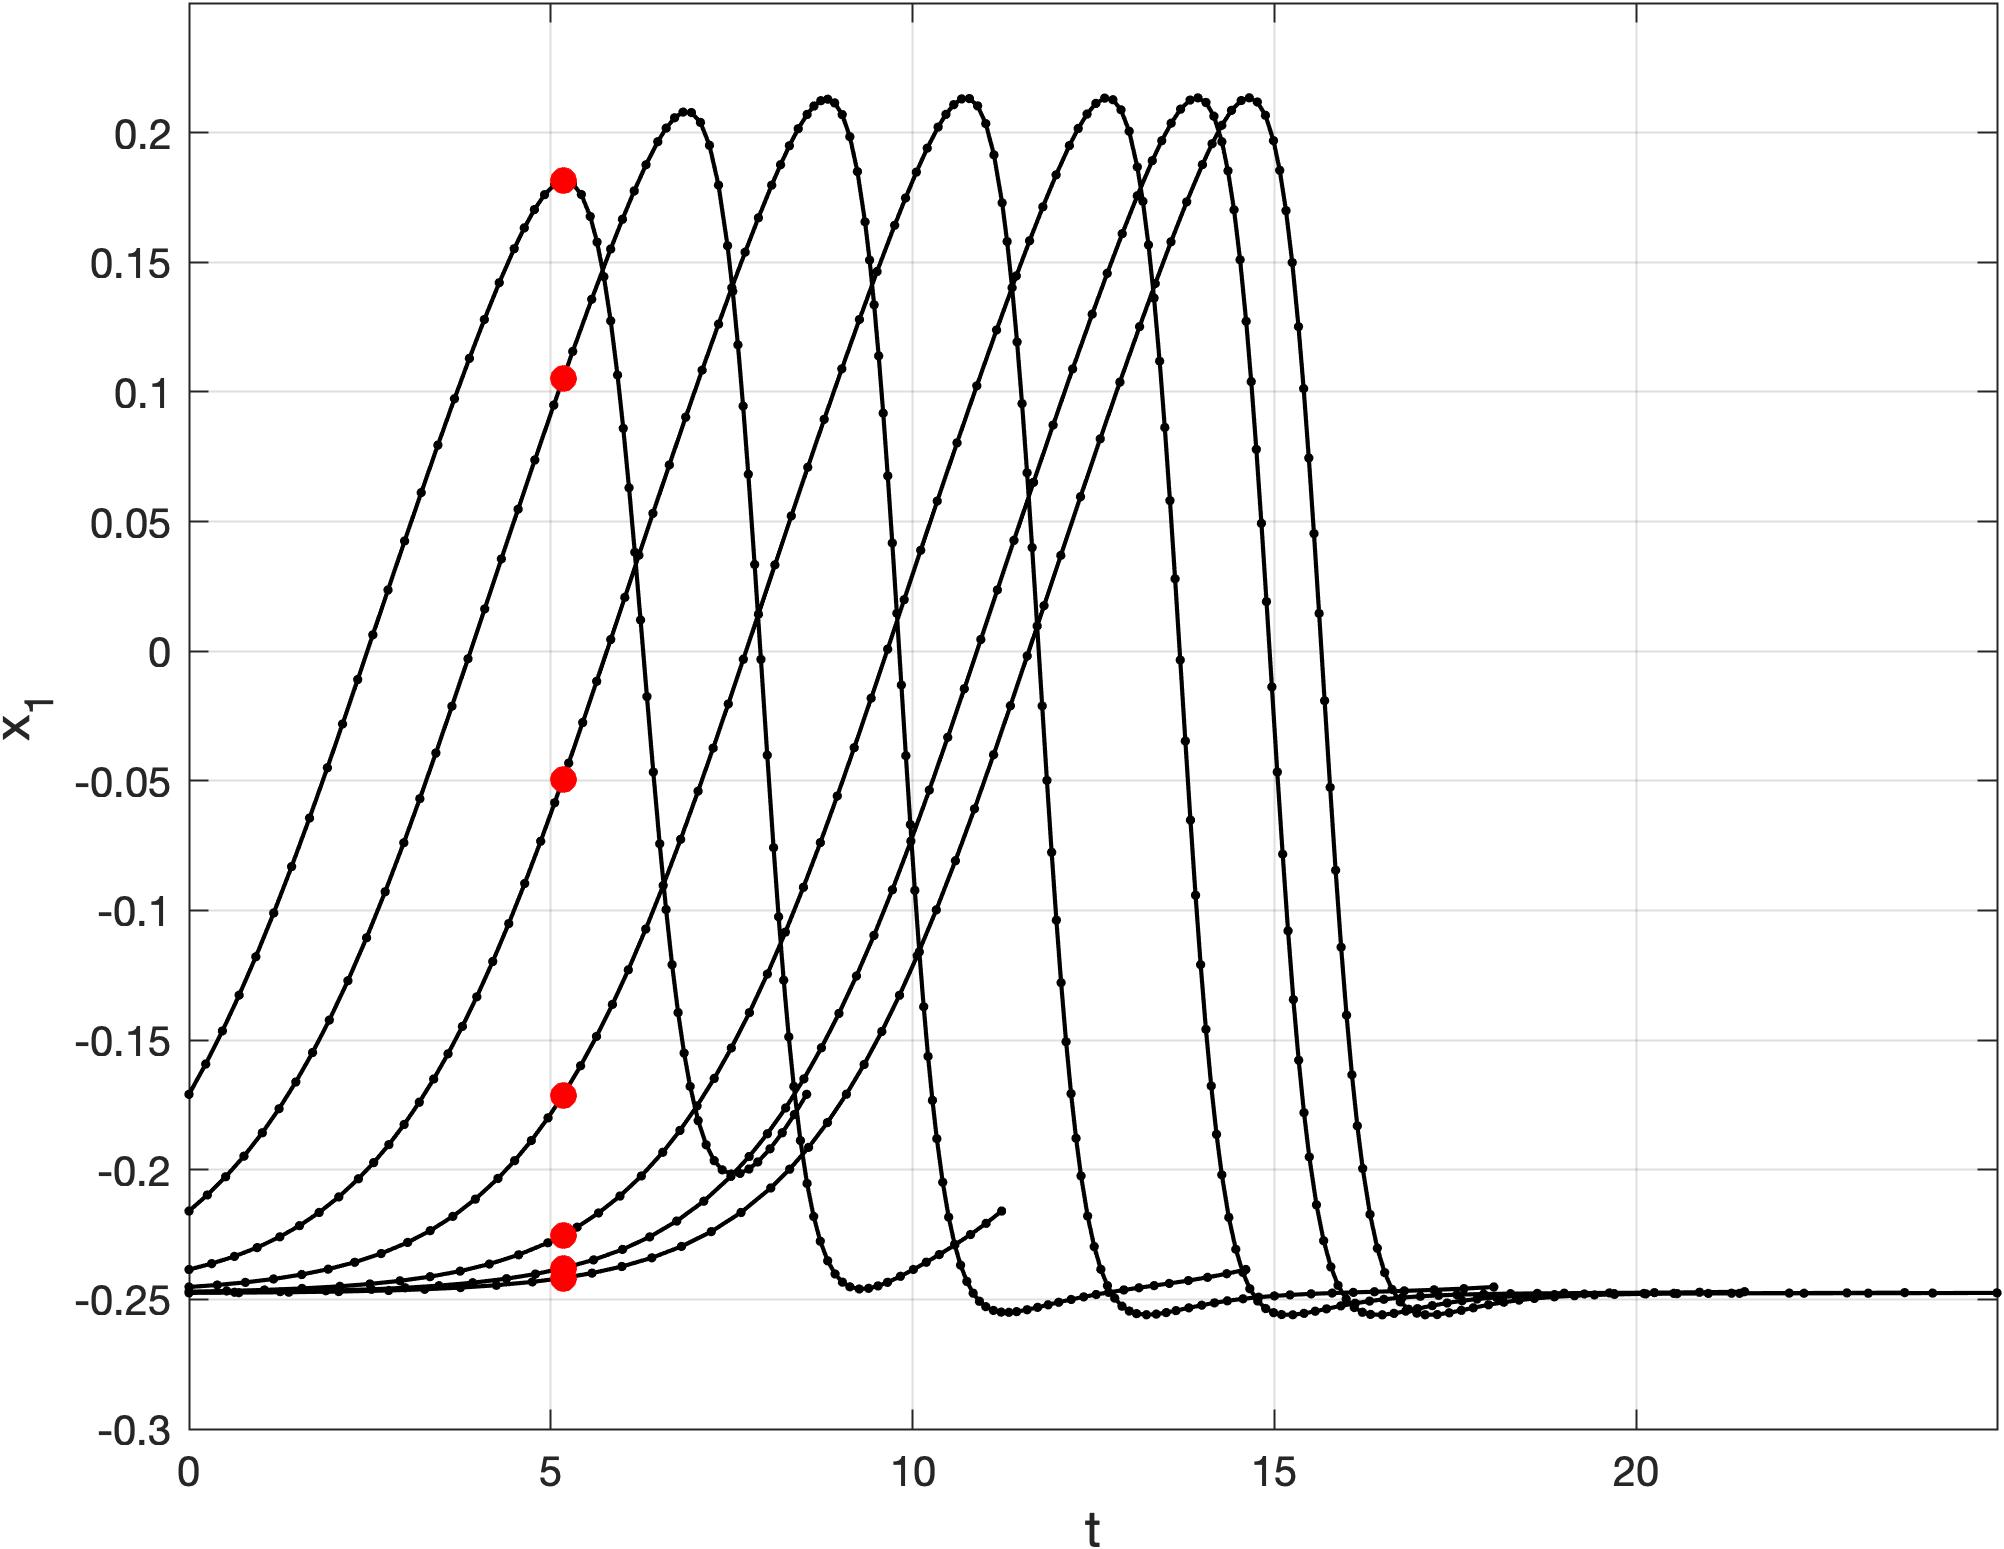
\includegraphics[width=4in]{Figures/Section7_4_2.jpg}
\caption{Time histories for labeled periodic orbits found during continuation using the code in Sect.~\ref{sec: Tracking and constraining orbit maxima} with points at $t=5.17$ highlighted using red disks.}
\label{fig: Section7_4_2}
\end{figure}

To track a local maximum in $x_1$, you execute the commands
\begin{lstlisting}[language=coco-highlight,frame=lines]
>> prob = coco_set_parival(prob, 'xtrs', 0);
>> coco(prob, 'new_po_run2', [], {'p1' 'po.period', 'trs', 'xrs'}, [-1 1]);

    STEP   DAMPING               NORMS              COMPUTATION TIMES
  IT SIT     GAMMA     ||d||     ||f||     ||U||   F(x)  DF(x)  SOLVE
   0                          9.01e-04  1.56e+01    0.0    0.0    0.0
   1   1  1.00e+00  2.71e-02  4.67e-05  1.56e+01    0.0    0.1    0.0
   2   1  1.00e+00  6.03e-04  2.37e-08  1.56e+01    0.0    0.2    0.0
   3   1  1.00e+00  3.05e-07  6.08e-15  1.56e+01    0.0    0.2    0.0

 STEP    ...   LABEL  TYPE            p1    po.period          trs          xrs
    0    ...       1  EP     -1.8570e-02   8.5271e+00   5.1859e+00   1.8133e-01
   10    ...       2         -1.4056e-02   1.0854e+01   6.6562e+00   2.0665e-01
   20    ...       3         -1.3254e-02   1.3805e+01   8.3568e+00   2.1255e-01
   30    ...       4         -1.3168e-02   1.6801e+01   1.0046e+01   2.1332e-01
   40    ...       5         -1.3158e-02   1.9828e+01   1.1748e+01   2.1342e-01
   50    ...       6  EP     -1.3156e-02   2.2872e+01   1.3458e+01   2.1343e-01
\end{lstlisting}
The results of the computation are visualized using the following commands (cf.\ Fig.~\ref{fig: Section7_4_3}).
\begin{lstlisting}[language=coco-highlight,frame=lines]
>> figure(2)
>> clf
>> hold on
>> coco_plot_sol('new_po_run2', '', 't', 'x')
>> tx = coco_bd_vals('new_po_run2', 'all', {'trs', 'xrs'});
>> plot(tx(1,:), tx(2,:), 'ro', 'MarkerFaceColor', 'r');
>> hold off
>> grid on
>> box on
>> axis([0 inf -0.3 0.25])
\end{lstlisting}
\begin{figure}[h]
\centering
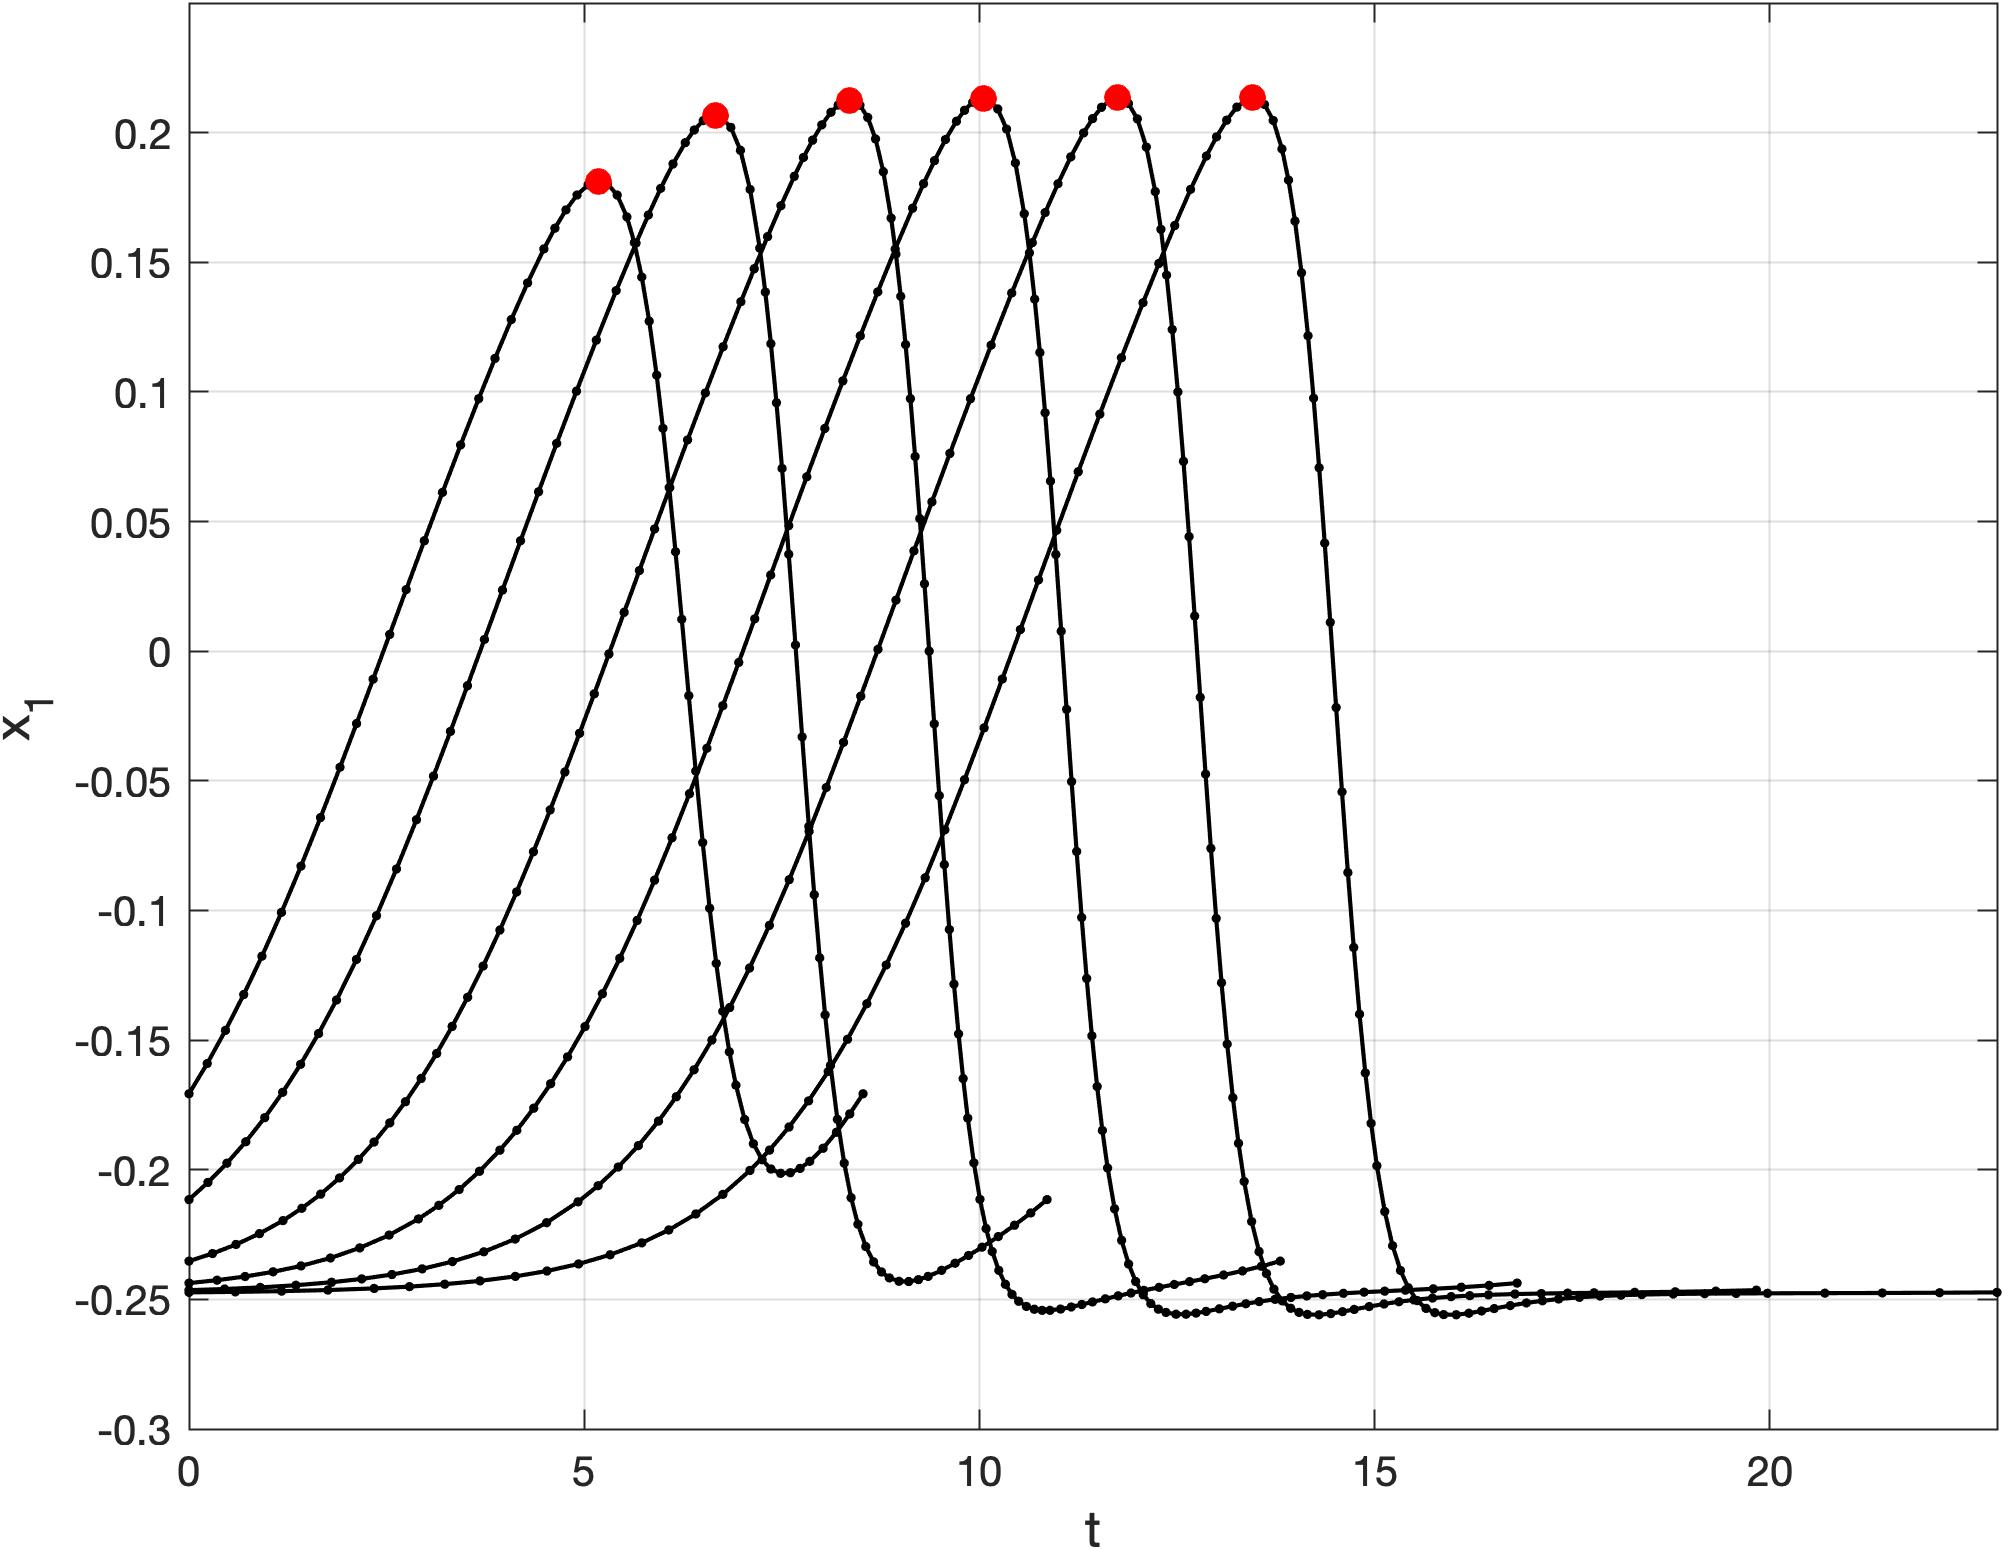
\includegraphics[width=4in]{Figures/Section7_4_3.jpg}
\caption{Time histories for labeled periodic orbits found during continuation using the code in Sect.~\ref{sec: Tracking and constraining orbit maxima} with a family of local maxima highlighted using red disks.}
\label{fig: Section7_4_3}
\end{figure}

Finally, you decide to continue along a family of periodic orbits for which the local maximum in $x_1$ is held fixed at its initial value of $x_1$. This is accomplished using the following command, in which $p_2$ is also allowed to vary.
\begin{lstlisting}[language=coco-highlight,frame=lines]
>> coco(prob, 'new_po_run3', [], {'p1' 'po.period', 'trs', 'p2'}, [-1 1]);

    STEP   DAMPING               NORMS              COMPUTATION TIMES
  IT SIT     GAMMA     ||d||     ||f||     ||U||   F(x)  DF(x)  SOLVE
   0                          9.01e-04  1.67e+01    0.0    0.0    0.0
   1   1  1.00e+00  2.72e-02  4.70e-05  1.67e+01    0.0    0.1    0.0
   2   1  1.00e+00  2.18e-03  2.98e-08  1.67e+01    0.0    0.2    0.0
   3   1  1.00e+00  1.29e-06  8.48e-15  1.67e+01    0.0    0.2    0.0
   4   1  1.00e+00  1.36e-13  1.22e-15  1.67e+01    0.0    0.3    0.0

 STEP    ...   LABEL  TYPE            p1    po.period          trs           p2
    0    ...       1  EP     -1.8581e-02   8.5288e+00   5.1868e+00   5.9951e+00
   10    ...       2         -1.1092e-02   1.0616e+01   6.6250e+00   7.3292e+00
   20    ...       3         -9.2076e-03   1.3509e+01   8.4001e+00   7.9542e+00
   30    ...       4         -8.9274e-03   1.6502e+01   1.0138e+01   8.0823e+00
   40    ...       5         -8.8852e-03   1.9524e+01   1.1870e+01   8.1027e+00
   50    ...       6  EP     -8.8790e-03   2.2560e+01   1.3608e+01   8.1058e+00
\end{lstlisting}
The results of this computation are visualized using the following commands (cf.\ Fig.~\ref{fig: Section7_4_4}).
\begin{lstlisting}[language=coco-highlight,frame=lines]
>> figure(3)
>> clf
>> hold on
>> coco_plot_sol('new_po_run3', '', 't', 'x')
>> tx = coco_bd_vals('new_po_run3', 'all', {'trs', 'xrs'});
>> plot(tx(1,:), tx(2,:), 'ro', 'MarkerFaceColor', 'r');
>> hold off
>> grid on
>> box on
>> axis([0 inf -0.3 0.25])
\end{lstlisting}
\begin{figure}[h]
\centering
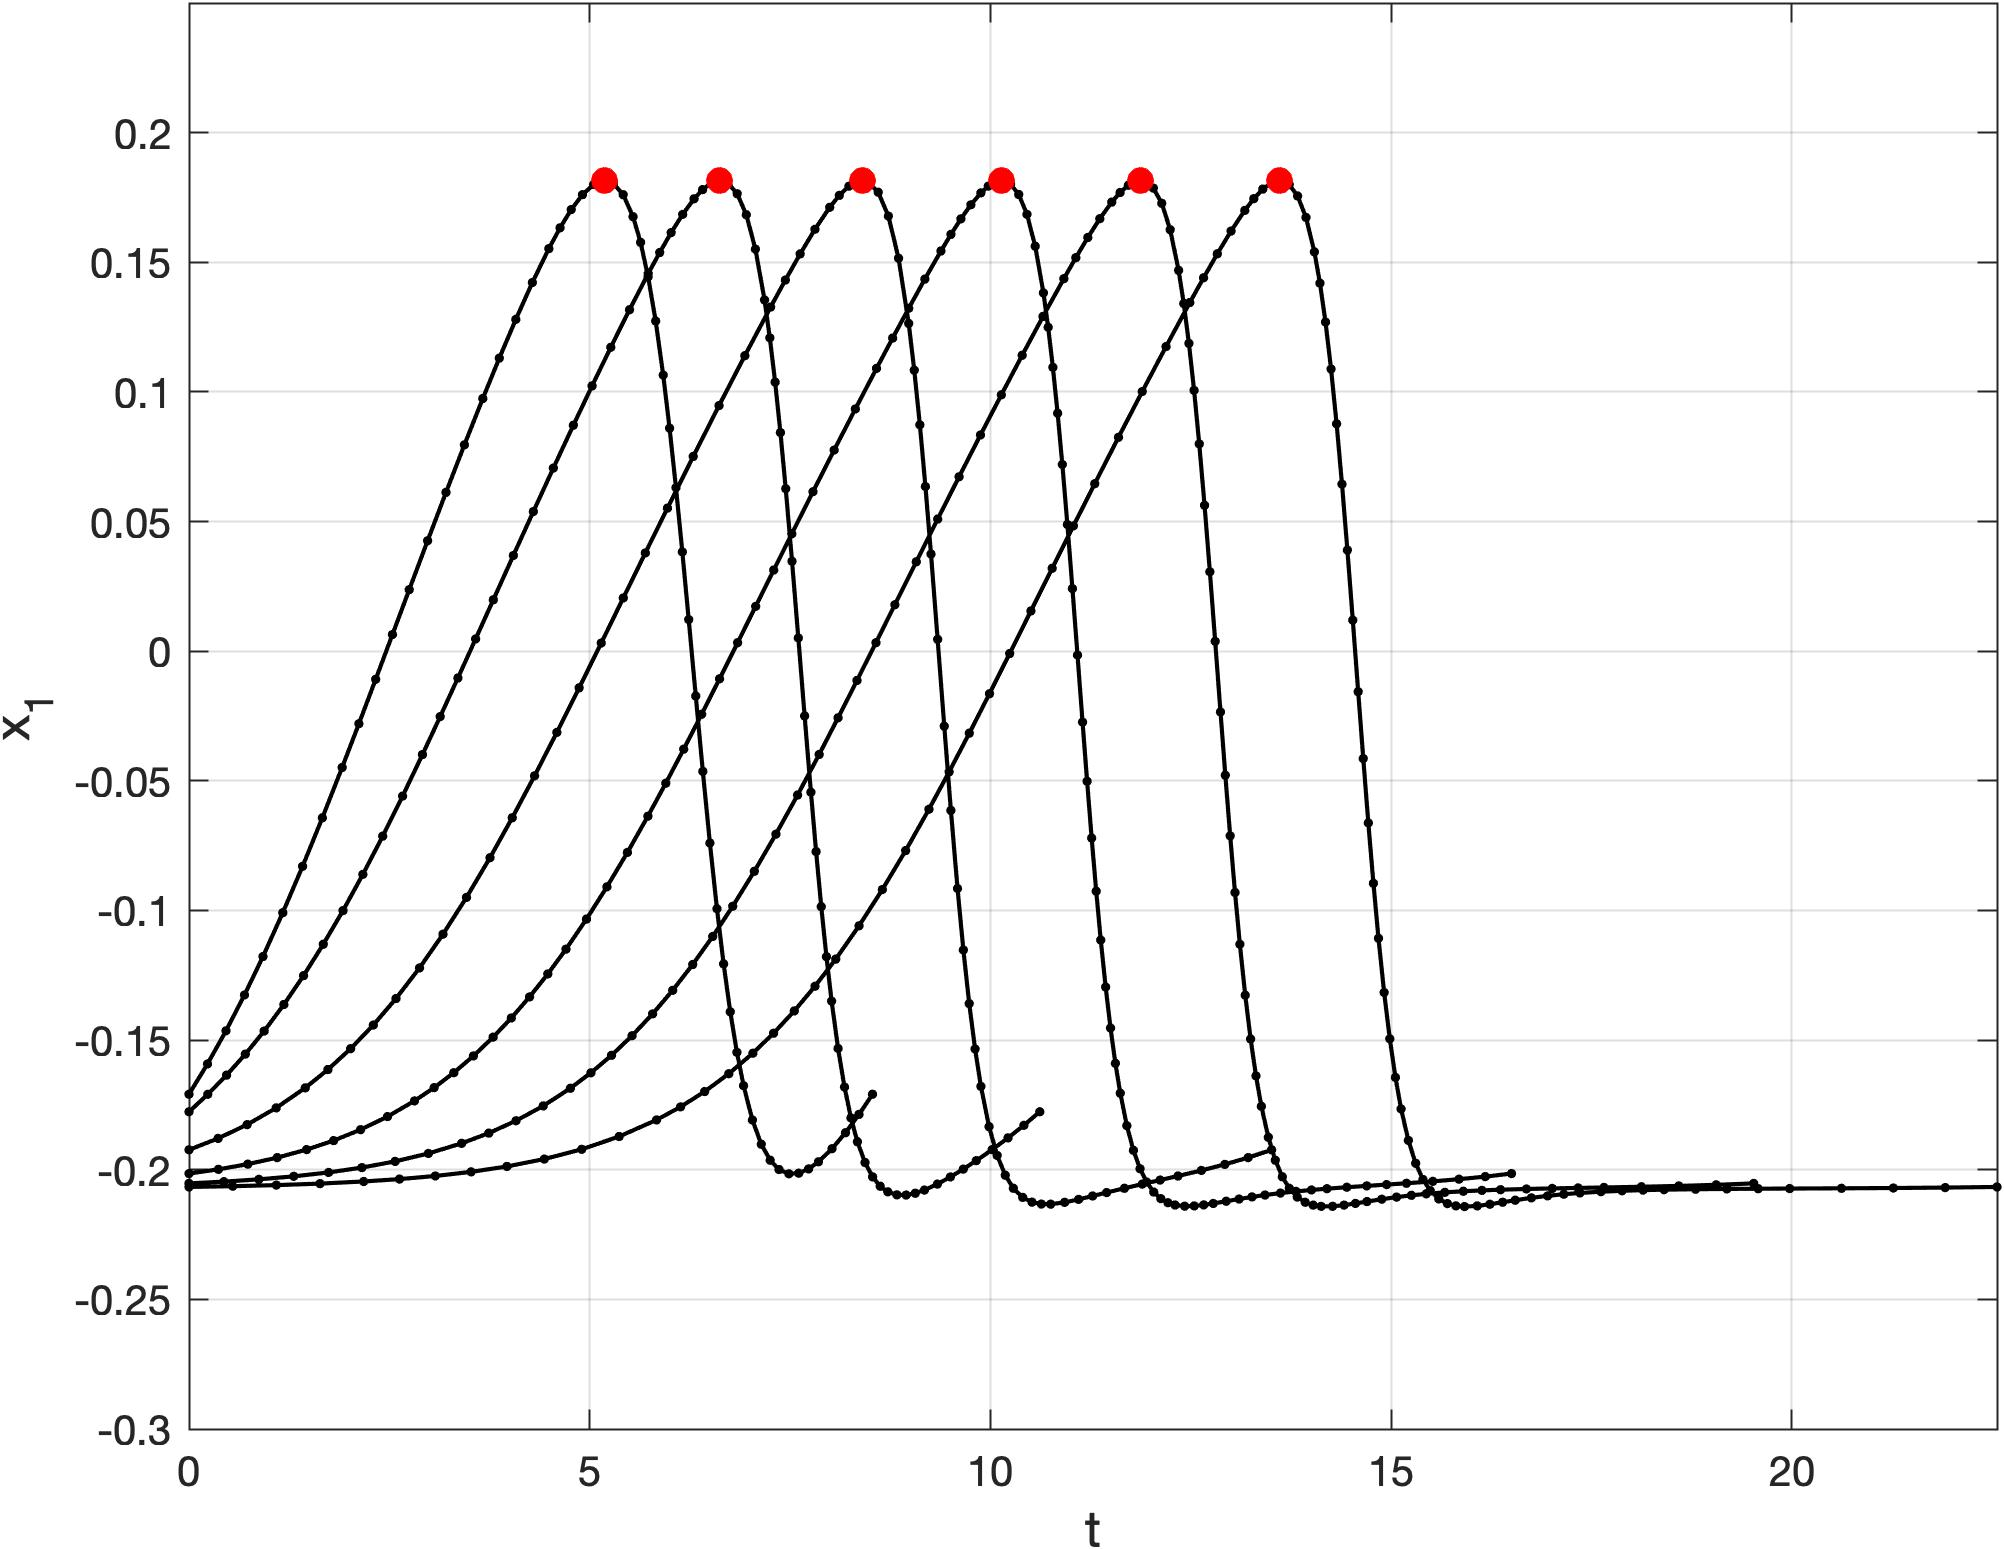
\includegraphics[width=4in]{Figures/Section7_4_4.jpg}
\caption{Time histories for labeled periodic orbits found during continuation using the code in Sect.~\ref{sec: Tracking and constraining orbit maxima} with a family of local maxima highlighted using red disks.}
\label{fig: Section7_4_4}
\end{figure}

\section{Outlook}
As demonstrated in the previous section on user-initiated enhancements, \textsc{coco} is expandable and not bound by a fixed set of predefined functionalities. The examples have barely scratched the surface of what is possible. They have also purposely stuck to a tight syntax, in the course of which some of the more exciting features may have been hidden from view.

Chances are that you have already thought of things you would like to do that don't appear straightforward within the framework presented in this tutorial. You may be inclined to ask whether a solution already exists. You may wonder how onerous an effort it might be to implement a solution when one does not appear available. 

As the saying goes about a free lunch, be prepared for a demanding but highly rewarding ride. There is no straight path that fits all. Perhaps you can find examples that resemble your use case among the demos included with each of the \mcode{'ep'}, \mcode{'coll'}, and \mcode{'po'} toolboxes (see the \texttt{help} folder for the corresponding tutorial documentation). For a more systematic but longer journey, consider the textbook \emph{Recipes for Continuation} by Dankowicz and Schilder.



\end{document}
